% This must be in the first 5 lines to tell arXiv to use pdfLaTeX, which is strongly recommended.
\pdfoutput=1
% In particular, the hyperref package requires pdfLaTeX in order to break URLs across lines.

\documentclass[11pt]{article}

% Change "review" to "final" to generate the final (sometimes called camera-ready) version.
% Change to "preprint" to generate a non-anonymous version with page numbers.
\usepackage[table,xcdraw]{xcolor}

% \usepackage[review]{acl}
\usepackage[]{acl}
\usepackage{listings}
\usepackage{multirow}
\usepackage{minted}
\usepackage{amssymb}
\usepackage{booktabs}
\usepackage{subcaption}
\usepackage{makecell}
\renewcommand\lstlistingname{Algorithm}
% \usepackage{lipsum}   % for filler text
\usepackage{etoolbox}
\AtBeginEnvironment{quote}{\par\singlespacing\small}
\usepackage{setspace} % for \onehalfspacing and \singlespacing macros
\newcommand{\gemini}{Gemini-1.0-Pro\xspace}
% \newcommand{\whitespace}{EWS\xspace}
\newcommand{\rf}{RF\xspace}
\newcommand{\trd}{TRD\xspace} % text repetition detection
\newcommand{\mtr}{MTR\xspace} 

% Standard package includes
\usepackage{times}
\usepackage{latexsym}
\newcommand{\ms}{MS MARCO\xspace}
\newcommand{\rp}{RPP\xspace}
\newcommand{\rpp}{RPP\xspace}
\newcommand{\mrs}{MRS\xspace}
\newcommand{\mrses}{MRSes\xspace}

\newcommand{\nwc}{NWC\xspace}
% \newcommand{\nwc}{NWC\xspace}

\usepackage{algorithm}
\usepackage{algpseudocode}
\usepackage{amsmath}


% For proper rendering and hyphenation of words containing Latin characters (including in bib files)
\usepackage[T1]{fontenc}
% For Vietnamese characters
% \usepackage[T5]{fontenc}
% See https://www.latex-project.org/help/documentation/encguide.pdf for other character sets

% This assumes your files are encoded as UTF8
\usepackage[utf8]{inputenc}
\usepackage{xspace}
\usepackage{amsmath}
\newcommand{\webqsp}{WebQSP\xspace}
% \newcommand{\ours}{RAPOLL\xspace}
% \newcommand{\ours}{RAPGeT\xspace}
\newcommand{\raggen}{RAG-GP\xspace}
\newcommand{\ragtem}{RAG-CT\xspace}
\newcommand{\nonrag}{Non-RAG\xspace}
\newcommand{\mtgen}{MT-GP\xspace}
\newcommand{\mttem}{MT-CT\xspace}
\newcommand{\hm}{$H$\xspace} % harmonic mean 

% \newcommand{\nrr}{NRR\xspace}
\newcommand{\rr}{RR\xspace}

\newcommand{\wds}{WebQSP\xspace}
\newcommand{\mds}{MS MARCO\xspace}
\newcommand{\mac}{MAC\xspace}

% \newcommand{\gem2}{Gemma-2B\xspace}
% \newcommand{\gem7}{Gemma-7B\xspace}
% \newcommand{\llama27}{Llama-2-7B\xspace}
% \newcommand{\llama213}{Llama-2-13B\xspace}
% \newcommand{\llama270}{Llama-2-70B\xspace}
% \newcommand{\llama38}{Llama-3-8B\xspace}
% \newcommand{\llama370}{Llama-3-70B\xspace}
% \newcommand{\mistral}{Mistral-7B\xspace}
% \newcommand{\phi}{Phi-3-mini\xspace}

\newcommand{\rap}{RAP\xspace}
\newcommand{\alg}{ReDA\xspace}

% \usepackage{algorithm2e}
\newcommand{\todo}[1]{\textcolor{red}{(#1)}}
\newcommand{\new}[1]{\textcolor{black}{#1}}

% This is not strictly necessary, and may be commented out,
% but it will improve the layout of the manuscript,
% and will typically save some space.
\usepackage{microtype}

% This is also not strictly necessary, and may be commented out.
% However, it will improve the aesthetics of text in
% the typewriter font.
\usepackage{inconsolata}

%Including images in your LaTeX document requires adding
%additional package(s)
\usepackage{graphicx}

\usepackage{algorithm}
\usepackage{algpseudocode}

\newtheorem{theorem}{Definition}


% If the title and author information does not fit in the area allocated, uncomment the following
%
%\setlength\titlebox{<dim>}
%
% and set <dim> to something 5cm or larger.

% \title{Evaluating the Effect of Repetition Penalty in Retrieval-Augmented Generation with Open-source Large Language Models}

% \title{The Perils of Repetition: Addressing Redundancy in Open-Source Large Language Models}

% \title{Balancing Repetition and Quality in Open-Source LLM Outputs:\\A Repetition-Aware Performance Evaluation Framework}
% \title{Balancing Repetition and Quality in Open-Source LLM Outputs:\\A Repetition-Aware Performance Evaluation Framework (\todo{to change title, to include RPP}}
% \title{Tuning Repetition Penalty Parameter (RPP) for Open-Source LLMs:\\A Repetition-Aware Performance Evaluation Framework\todo{Donghao's proposal}}
\title{RAP: A Metric for Balancing Repetition and Performance in \\Open-Source Large Language Models}
% \title{How to Suppress Repetition in Open-source LLMs: Tuning Repetition Panalty Parmeter}  % need more sounding title 

% Author information can be set in various styles:
% For several authors from the same institution:
% \author{Author 1 \and ... \and Author n \\
%         Address line \\ ... \\ Address line}
% if the names do not fit well on one line use
%         Author 1 \\ {\bf Author 2} \\ ... \\ {\bf Author n} \\
% For authors from different institutions:
% \author{Author 1 \\ Address line \\  ... \\ Address line
%         \And  ... \And
%         Author n \\ Address line \\ ... \\ Address line}
% To start a separate ``row'' of authors use \AND, as in
% \author{Author 1 \\ Address line \\  ... \\ Address line
%         \AND
%         Author 2 \\ Address line \\ ... \\ Address line \And
%         Author 3 \\ Address line \\ ... \\ Address line}


\author{
 \textbf{Donghao HUANG\textsuperscript{1,2}},
 \textbf{Thanh-Son NGUYEN\textsuperscript{3}},
 \textbf{Fiona LIAUSVIA\textsuperscript{3}},
 \textbf{Zhaoxia WANG\textsuperscript{1}}
%\\
%  \textbf{Fifth Author\textsuperscript{1,2}},
%  \textbf{Sixth Author\textsuperscript{1}},
%  \textbf{Seventh Author\textsuperscript{1}},
%  \textbf{Eighth Author \textsuperscript{1,2,3,4}},
%\\
%  \textbf{Ninth Author\textsuperscript{1}},
%  \textbf{Tenth Author\textsuperscript{1}},
%  \textbf{Eleventh E. Author\textsuperscript{1,2,3,4,5}},
%  \textbf{Twelfth Author\textsuperscript{1}},
%\\
%  \textbf{Thirteenth Author\textsuperscript{3}},
%  \textbf{Fourteenth F. Author\textsuperscript{2,4}},
%  \textbf{Fifteenth Author\textsuperscript{1}},
%  \textbf{Sixteenth Author\textsuperscript{1}},
%\\
%  \textbf{Seventeenth S. Author\textsuperscript{4,5}},
%  \textbf{Eighteenth Author\textsuperscript{3,4}},
%  \textbf{Nineteenth N. Author\textsuperscript{2,5}},
%  \textbf{Twentieth Author\textsuperscript{1}}
%\\
\\
 \textsuperscript{1}School of Computing and Information Systems, 
  Singapore Management University, Singapore \\
\textsuperscript{2}Research and Development, Mastercard, Singapore \\
% \textsuperscript{3}Social and Cognitive Computing, Institute of High Performance Computing (IHPC), \\Agency for Science, Technology and Research (A*STAR), Singapore\\
\textsuperscript{3}Institute of High Performance Computing (IHPC), \\Agency for Science, Technology and Research (A*STAR), Singapore\\
%  \textsuperscript{4}Affiliation 4,
%  \textsuperscript{5}Affiliation 5
%\\
% \small{
% \textbf{Correspondence:} \href{mailto:zxwang@smu.edu.sg}{zxwang@smu.edu.sg}
%  }
}

\begin{document}
\maketitle

\begin{abstract}
Large Language Models (LLMs) have significantly advanced natural language processing, but content repetition in open-source LLMs remains a critical challenge that adversely affects user experience. The repetition penalty parameter (\rpp) aims to mitigate this issue by preventing repeated content generation, but excessive use of \rpp can compromise the overall quality.
In this paper, we propose Repetition-Aware Performance (\rap), a novel evaluation metric that quantifies and integrates repetition penalty into the assessment of model performance, enabling tuning of \rpp. 
We evaluate our approach using twelve open-source LLMs, ranging from 2 billion to 70 billion parameters, tested on question answering and machine translation tasks across three datasets with varying prompting techniques. 
Experimental results show that RAP effectively tunes RPP, helping to identify a trade-off value that significantly reduces repetition while minimizing performance loss.
The code and the dataset of generated text can be accessed at \url{https://github.com/inflaton/rap}.
% Upon acceptance, we will release the code and the dataset of generated text, providing a valuable resource for further research on repetition detection and LLMs evaluation.

% Large Language Models (LLMs) have significantly advanced the field of natural language processing; however, the issue of content repetition in open-source LLMs remains a critical challenge, negatively affecting user experience. The repetition penalty parameter (\rpp) is designed to mitigate this issue by preventing the generation of repeated content, but excessive application of \rpp can compromise the overall quality of the generated text. 
%

% Additionally, we find that chat templates effectively reduce repetition, a strategy underused in LLM applications development. 
% We assess our approach using twelve LLMs, with sizes ranging from 2 billion to 70 billion parameters, tested on question answering and machine translation tasks, utilizing three datasets and varying prompting techniques.
% These techniques include both Retrieval-Augmented Generation (RAG) and non-RAG strategies, using generic prompt and chat template. 
% We evaluate twelve LLMs, with sizes ranging from 2 billion to 70 billion parameters, yielding insights into optimal parameter settings for minimizing repetition while maintaining quality.
%
% Experimental results show that increasing \rpp generally decreases performance, thus tuning \rpp to find the balance is important. 
% Our findings show that RAP can be used to effectively tune RPP, helping to identify a trade-off value that significantly reduces repetition while minimizing performance loss.
% We also find that chat templates effectively reduce repetition, a strategy underused in LLM applications development. 
% Upon acceptance, we will release the code and the dataset of generated text, providing a valuable resource for further research on repetition detection and LLMs evaluation.

% We also find that increasing \rpp generally reducing performance, therefore, having a balance approach is desireable, that can be tuned using our proposed metric, \rap. 
% Upon acceptance, we will make the source code and all experimental data publicly available, including a substantial corpus of text generated by open-source LLMs. This dataset will serve as a valuable resource for future research in developing repetition detection methods and evaluating LLM capabilities in question-answering tasks.


% Large Language Models (LLMs) have significantly advanced natural language processing, yet content repetition issue in open-source LLMs remains a challenge and negatively impacts user experience in applications like conversational chatbots. Repetition penalty parameter (\rpp) is designed to stop LLMs from generating repeated content. However, excessive use of \rpp can impact the quality of the generated text. In this paper, we propose 

% \todo{to revise, add findings, add MT}
% We propose Repetition-Aware Performance (\rap) metric, to investigate the impact of repetition penalty parameter (\rp) on the quality of responses generated by open-source LLMs. RAPGeT incorporates a novel metric, the repetition factor (RF), to quantify the repetition penalty into model's performance. This enable identifying the trade-off between repetition and overall quality.
% Our evaluation on two question-answering datasets (\webqsp and \ms), using both Retrieval-Augmented Generation (RAG) and non-RAG approaches, provides insights into optimal parameter settings. 
% We analyze nine LLMs with sizes ranging from 2 billion to 70 billion parameters, providing insights on reducing repetition while maintaining quality in open-source LLMs.
% Our findings show that an optimal balance between repetition suppression and response quality can be achieved with careful tuning of the RPP.
% Upon acceptance, we will publish the source code and our experiment results. This data can be used for future tasks such as designing repetition detection methods or evaluating LLMs’ capabilities in QA tasks.


% Large Language Models (LLMs) have significantly advanced natural language processing, yet content repetition issue in open-source LLMs remains a challenge and negatively impacts user experience in applications like conversational chatbots. The \textit{repetition penalty parameter} (\rp) mitigates this issue by penalizing frequent tokens but can lead to incomplete responses if applied stringently.
% %
% In this paper, we propose Repetition-Aware Performance Evaluation for Generated Text (\ours) framework, to investigate \rp effect on the quality of responses generated by open-source LLMs.
% We define the problem of repetition penalty detection and introduce the \textit{repetition factor}, a novel metric that quantifies repetition penalty on performance, allowing us to identify the trade-off between repetition and overall quality.
% Our evaluation on two question-answering datasets (\webqsp and \ms), using both Retrieval-Augmented Generation (RAG) and non-RAG approaches, provides insights into optimal parameter settings. 
% We analyze nine LLMs with sizes ranging from 2 billion to 70 billion parameters, providing insights on reducing repetition while maintaining quality in open-source LLMs.
% Our findings show that an optimal balance between repetition suppression and response quality can be achieved with careful tuning of the RPP. For instance, models like Llama-2-7B and Llama-3-8B experience significant improvements in repetition-aware performance scores when using the RAPGeT framework, demonstrating the effectiveness of our approach. 
% Upon acceptance, we will publish the source code and our experiment results. This data can be used for future tasks such as designing repetition detection methods or evaluating LLMs’ capabilities in QA tasks. 

% Large Language Models (LLMs) have significantly advanced natural language processing, yet content repetition issue in open-source LLMs remains a challenge and negatively impacts user experience in applications
% We propose Repetition-Aware Performance Evaluation for Generated Text (\ours) framework, to investigate \rp effect on the quality of responses generated by open-source LLMs.
% We define the problem of repetition penalty detection and introduce the \textit{repetition factor}, a novel metric that quantifies repetition penalty on performance, allowing us to identify the trade-off between repetition and overall quality.
% Our evaluation on two question-answering datasets (\webqsp and \ms), using both Retrieval-Augmented Generation (RAG) and non-RAG approaches, provides insights into optimal parameter settings. 
% We analyze nine LLMs with sizes ranging from 2 billion to 70 billion parameters, providing insights on reducing repetition while maintaining quality in open-source LLMs.
% Our findings show that an optimal balance between repetition suppression and response quality can be achieved with careful tuning of the RPP. For instance, models like Llama-2-7B and Llama-3-8B experience significant improvements in repetition-aware performance scores when using the RAPGeT framework, demonstrating the effectiveness of our approach. 
% Upon acceptance, we will publish the source code and our experiment results. This data can be used for future tasks such as designing repetition detection methods or evaluating LLMs’ capabilities in QA tasks. 


% This paper introduces the Repetition-Aware Performance Evaluation for Generated Text (RAPGeT) framework to address content repetition in open-source Large Language Models (LLMs), particularly impacting user experience in conversational applications. RAPGeT incorporates a novel metric, the repetition factor (RF), to quantify the repetition penalty into model's performance and mitigate repetition through the adjustment of the repetition penalty parameter (RPP). Our comprehensive evaluation across two major question-answering datasets—WebQSP and MS MARCO—utilizing both Retrieval-Augmented Generation (RAG) and non-RAG approaches, reveals that fine-tuning RPP effectively balances repetition suppression with response quality. This framework demonstrates significant performance improvements in models like Llama-2-7B and Llama-3-70B, illustrating its potential to enhance the quality of responses in LLMs without sacrificing content richness.



% We propose Repetition-Aware Performance Evaluation for Generated Text (\ours) framework, to investigate the impact of repetition penalty parameter (\rp) on the quality of responses generated by open-source LLMs. RAPGeT incorporates a novel metric, the repetition factor (RF), to quantify the repetition penalty into model's performance. This enable identifying the trade-off between repetition and overall quality.
% Our evaluation on two question-answering datasets (\webqsp and \ms), using both Retrieval-Augmented Generation (RAG) and non-RAG approaches, provides insights into optimal parameter settings. 
% We analyze nine LLMs with sizes ranging from 2 billion to 70 billion parameters, providing insights on reducing repetition while maintaining quality in open-source LLMs.
% Our findings show that an optimal balance between repetition suppression and response quality can be achieved with careful tuning of the RPP.
% Upon acceptance, we will publish the source code and our experiment results. This data can be used for future tasks such as designing repetition detection methods or evaluating LLMs’ capabilities in QA tasks. 

% Our findings show that an optimal balance between repetition suppression and response quality can be achieved with careful tuning of the RPP. For instance, models like Llama-2-7B and Llama-3-8B experience significant improvements in repetition-aware performance scores when using the RAPGeT framework, demonstrating the effectiveness of our approach. 

% Our findings show that an optimal balance between repetition suppression and response quality can be achieved with careful tuning of the RPP. For instance, models like Llama-2-7B and Llama-3-8B experience significant improvements in repetition-aware performance scores when using the RAPGeT framework, demonstrating the effectiveness of our approach. 
% Upon acceptance, we will publish the source code and our experiment results. This data can be used for future tasks such as designing repetition detection methods or evaluating LLMs’ capabilities in QA tasks. 
\end{abstract}

% \keywords{Large Language Models (LLMs), Natural Language Processing (NLP), Repetition Penalty Parameter (RPP), Repetition-Aware Performance Evaluation (RAPGeT), Repetition Factor (RF), Open-Source LLMs, Content Repetition, Question-Answering, Retrieval-Augmented Generation (RAG), NHyperparameter Tuning, Knowledge Base QA (KBQA), Open-Ended QA (OEQA), Text Generation, Repetition Detection Methods}

% Long Papers
% Long papers must describe substantial, original, completed and unpublished work. Wherever appropriate, concrete evaluation and analysis should be included. Long papers may consist of:

% up to eight (8) pages of content
% plus up to one page for limitations (required, see below) and optionally ethical considerations
% plus unlimited pages of references
% Submissions that exceed the length requirements, or are missing a limitations section, will be desk rejected.

% \todo{
% \begin{itemize}
%     \item draw a figure of the whole paper  
% \end{itemize}
% }

\section{Introduction}
The rapid advancement of Large Language Models (LLMs) has transformed natural language processing, enabling remarkable text generation and comprehension capabilities. However, open-source LLMs often generate repetitive content, leading to extensive empty lines or recurring sentences, which undermines text quality and fluency. This is particularly problematic in tasks requiring coherent and contextually relevant responses, such as conversational chatbots. To address this, the \textit{repetition penalty parameter} (\rp) is employed during the sampling process to reduce redundant outputs by penalizing previously seen tokens \cite{Keskar2019CTRLAC}. While effective, excessive application of \rp can result in incomplete or fragmented responses, ultimately diminishing user satisfaction.

\begin{figure}
    \centering
    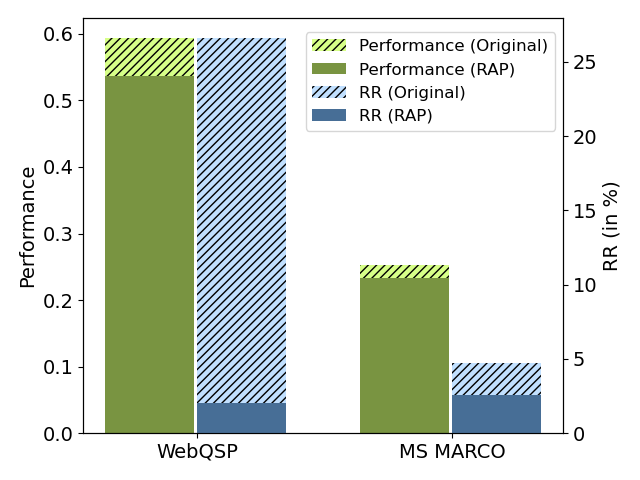
\includegraphics[width=1\linewidth]{image/chart_00_w_legend_Meta-Llama-3-8B-Instruct(RAG - Generic Prompt)_2.png}
    \caption{
    Best performance (F1 for WebQSP, BERT-F1 for MS MARCO) when tuning \rpp using original evaluation metrics (Original) and our proposed repetition-aware performance metric (\rap). \rap helps find \rpp values that minimally reduce performance while significantly lowering repetition ratio (\rr). Result is from Llama-3-8B (RAG-Generic Prompt).}
    \label{fig:hook}
    \vspace{-1.2em}
\end{figure}

% \todo{to rewrite the introduction, remove RF} 
% This paper investigates the intricate interplay between \rp and its impact on generated text. Typically, parameters like \textit{temperature} and \textit{top-k sampling} are optimized through hyperparameter tuning methods such as random or grid search. These methods involve running models with varied parameter values and selecting the best evaluation scores. However, they fail for tuning \rp because traditional metrics like precision, recall, and BLEU scores \cite{papineni2002bleu} overlook repetition. 
This paper explores the relationship between \rpp and its effect on generated text. While parameters like \textit{temperature} and \textit{top-k sampling} are optimized using methods like random or grid search, these fail for tuning \rpp since traditional metrics, such as precision and BLEU scores \cite{papineni2002bleu}, overlook repetition.
% \new{
To address this, we propose a metric called \textbf{R}epetition-\textbf{A}ware \textbf{P}erformance (\rap), which quantifies repetition and penalizes it in the model’s performance evaluation, allowing for the tuning of \rpp. 
Figure \ref{fig:hook} illustrates tuning \rpp for Llama-3-8B using the original evaluation metrics (Original) and our proposed metric. For the WebQSP dataset \cite{yih2016value}, repetition ratio (\rr) is reduced by 93.1\% but the performance only drops by 3.7\%. For the MS MARCO dataset \cite{huang2024performance}, \rr drops by 73.9\% with only 3.7\% of performance drop. Tuning \rpp using \rap can significantly reduce the \rr with minimal performance loss. More examples can be found in Appendix (\ref{sec:how_severe}).

% Figure \ref{fig:hook} shows an example when tuning \rpp for Llama-3-8B using the original evaluation metrics (Original) and our proposed metric (\rap). \rap helps find \rpp values that minimally reduce performance  while significantly lowering repetition ratio. For WebQSP dataset \cite{}, the performance reduces 3.7\%, but the repetition ratio (\rr) reduces 93.1\%. These numbers for MS MARCO dataset \cite{} are 3.7\% and 73.9\%. 
%
% Figure \ref{fig:hook} shows an example of tuning \rpp for Llama-3-8B when using the original evaluation metrics (Original) and our proposed metric. \rap helps in identifying \rpp values that minimize performance reduction while substantially decreasing the repetition ratio (\rr). For the WebQSP dataset \cite{yih2016value}, performance drops by 3.7\%, but the repetition ratio decreases by 93.1\%. For the MS MARCO dataset \cite{huang2024performance}, the performance reduction is 3.7\%, with a 73.9\% decrease in repetition ratio.
%
To compute \rap, we introduce an efficient algorithm called \alg -- Repetition Detection Algorithm--designed to identify all repeating patterns, including non-word character (\nwc) and text repetitions, along with their corresponding repetition lengths. Additionally, we define the repetition ratio (\rr), which measures the proportion of repeated content relative to the total text length. \rr is applied to penalize the model’s performance using a cubic penalty formula, as detailed in Section \ref{sec:method}. Figure \ref{fig:overall} illustrates computing \rap with a running example. 
% Although the accuracy is 100\%, the content has many repeated text that results in reducing the performance to 24.63\%. 
Although the accuracy is 100\%, the content contains many repeated elements, resulting in a low RAP score of 24.63\%.
% }
% quantify repetition by integrating \rf into the model’s evaluation. Using an efficient method based on regular expressions, we measure repetition in LLM responses and compute \rf to penalize performance according to repetition levels. Figure \ref{fig:overall} illustrates \ours with a running example. Although the accuracy is 100\%, the content has many repeated text that results in reducing the \textit{repetition-aware performance} (\rap) to 49.18\%. 
% The repetition factor, combined with a tailored algorithm for detecting repetition patterns, forms a comprehensive framework for optimizing performance while suppressing redundancy. Details are in Section \ref{sec:method}.

% we propose a novel metric called \textit{repetition factor} (\rf), calculated based on the total length of repeated content in the generated text. By incorporating \rf into evaluation metrics, we effectively penalize performance based on the level of repetition in the response.

%
% We propose a framework, namely Repetition-Aware Performance Evaluation for Generated Text (\ours), to quantify repetition by integrating \rf into the model’s evaluation. Using an efficient method based on regular expressions, we measure repetition in LLM responses and compute \rf to penalize performance according to repetition levels. Figure \ref{fig:overall} illustrates \ours with a running example. Although the accuracy is 100\%, the content has many repeated text that results in reducing the \textit{repetition-aware performance} (\rap) to 49.18\%. 
% The repetition factor, combined with a tailored algorithm for detecting repetition patterns, forms a comprehensive framework for optimizing performance while suppressing redundancy. Details are in Section \ref{sec:method}.
%
% We perform a thorough evaluation of nine open-source LLMs with sizes ranging from 2 billion to 70 billion parameters. Our experiments encompass two distinct question-answering (QA) tasks: knowledge base question answering (KBQA) and open-ended question answering (OEQA). For KBQA, we utilize the WebQSP dataset \cite{yih2016value}, where each answer comprises a list of entities from the Freebase knowledge graph. For OEQA, we employ the \ms\footnote{\url{https://microsoft.github.io/msmarco/}} dataset \cite{bajaj2016ms}, which includes real Bing questions and human-generated answers. Given that \webqsp requires entity lists as answers, we introduce an LLM-based evaluation method for KBQA. Specifically, we ask an LLM to extract answer-items (entities) from the generated text and mapping the predicted entities to the ground-truth entities. This approach allows us to use KBQA evaluation metrics, including precision, recall, and F1, as detailed in Section \ref{sec:gemini}. Additionally, we explore the impact of \rp on two prompting strategies: Retrieval-Augmented Generation (RAG)\cite{lewis2020retrieval} and non-RAG. Our study, which covers a diverse range of models, provides valuable insights into the optimal parameter values for balancing performance and repetition suppression in open-source LLMs.
%
\begin{figure*}
    \centering
    % 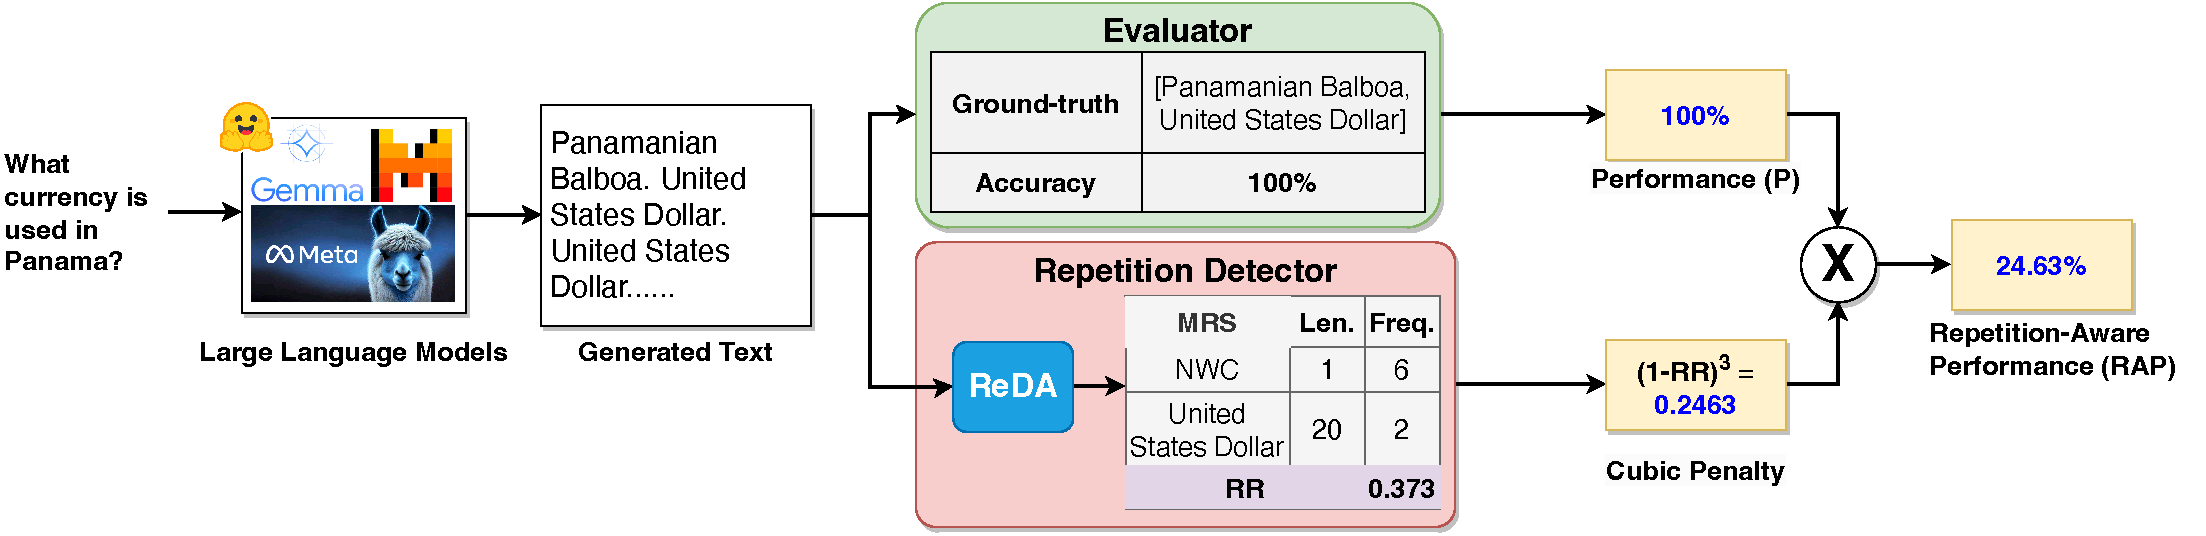
\includegraphics[width=\textwidth]{image/RAPGeT_v4.pdf}
    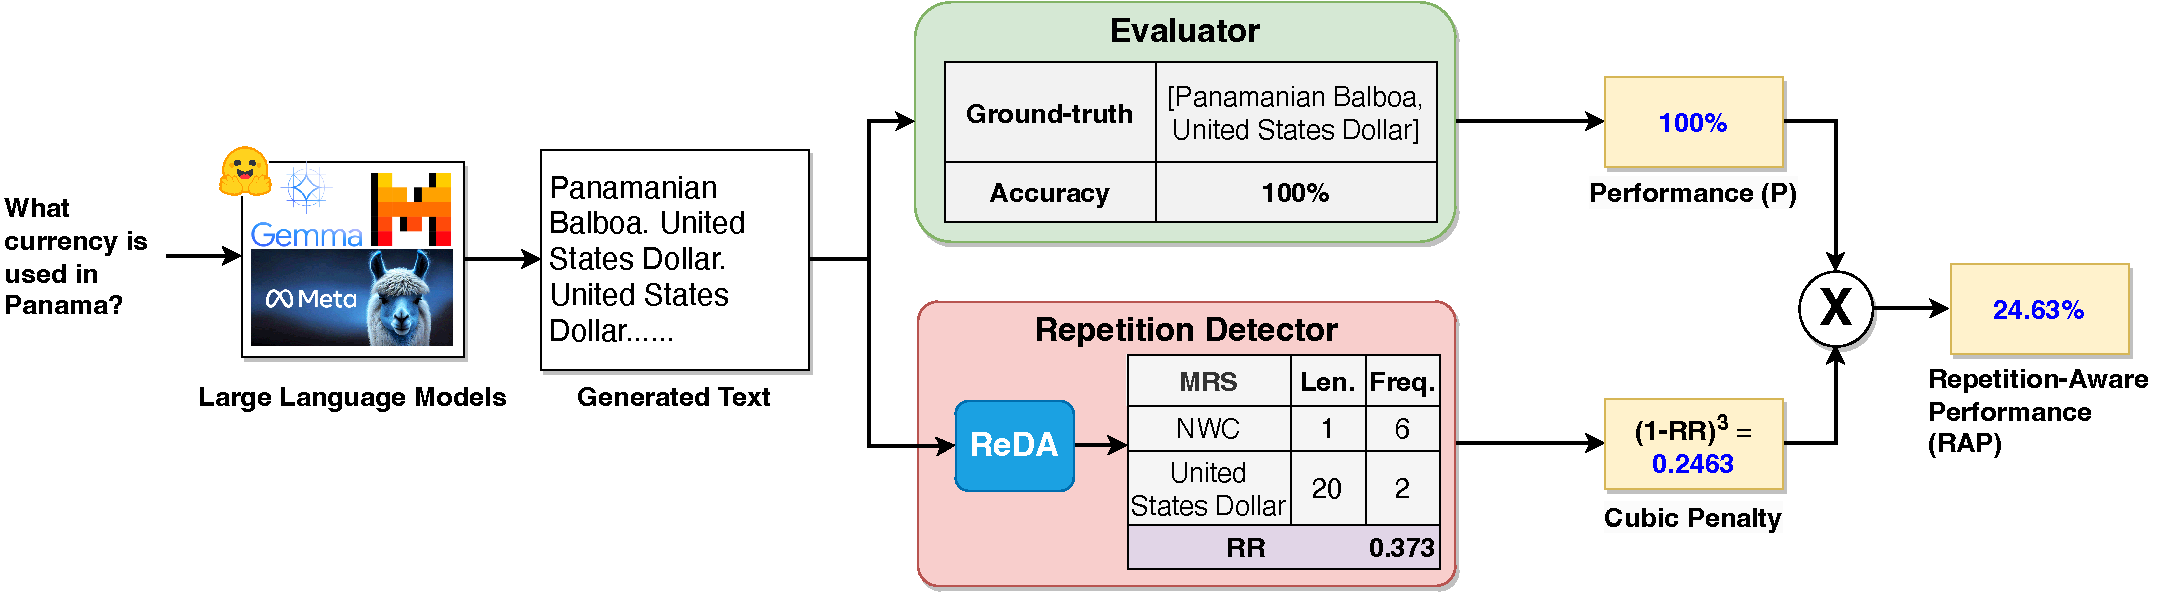
\includegraphics[width=\textwidth]{image/RAPGeT_v3-v5.2.pdf}
    \caption{Overall Methodology: \rap integrates the repetition penalty in the evaluation score. In the example, the generated text contains non-word characters (\nwc) repetition and text repetition. After penalization, the accuracy is reduced from 100\% to 24.63\%. \alg stands for Repetition Detection Algorithm.
    % Repetition-Aware Performance (\rap) integrates a repetition penalty into the evaluation score. In the illustration, the generated text contains non-word character (\nwc) repetition and text repetition, as shown in block (a). Here, \alg stands for the Repetition Detection Algorithm. After applying the repetition penalty, the performance is reduced from 100\% (without detecting repetition) to 24.63\% (after considering repetition). If no repetition is detected in block (a), the RAP score in block (c) will be the same as the performance obtained in block (b), which does not consider the repetition penalty.
    }
        \label{fig:overall}
\end{figure*}

We conduct experiments on three datasets encompassing question answering (including knowledge base question answering--KBQA-- and open-ended QA) and machine translation tasks.
% For question answering, we use \webqsp \cite{yih2016value} (knowledge base QA -- KBQA) and MS MARCO\footnote{\url{https://microsoft.github.io/msmarco/}} \cite{bajaj2016ms} (open-ended QA) datasets. For machine translation, we use \todo{MT-DATASET HERE!}. 
We evaluate twelve open-source LLMs ranging from 2 to 70 billion parameters. 
% For KBQA, answers are lists of entities from the Freebase knowledge graph. 
% As KBQA requires entity lists as answers, we introduce an LLM-based evaluation method for KBQA evaluation. We ask an LLM (\gemini) to extract entities from generated text and map them to ground-truth entities, enabling the use of KBQA metrics like precision, recall, and F1. 
We also examine the effect of repetition suppression for different prompting strategies including Retrieval-Augmented Generation (RAG) \cite{lewis2020retrieval} and non-RAG, combining with generic prompt and chat template.

Our study reveals that increasing \rpp typically reduces repetition but often results in performance degradation, highlighting the importance of tuning \rpp. The effects of \rpp differ across various models, datasets, and prompting techniques. Additionally, we find that using chat templates is effective in reducing repetition for QA task. Our experimental results demonstrate that \rap can effectively tune \rpp, helping to identify a trade-off value that significantly reduces repetition while minimizing performance loss.
These findings offer insights into optimizing \rpp for performance and repetition suppression in open-source LLMs.

This paper presents three key contributions. 
% \begin{itemize}
First, we propose \rap, a novel evaluation metric based on the repetition ratio that quantifies and integrates repetition issues into model performance, enabling the tuning of hyperparameters such as \rpp. We also develop an efficient Repetition Detection Algorithm (ReDA) algorithm for detecting both \nwc and text repetition, addressing  the key challenge in open-source LLMs. 
% Second, we present an LLM-based evaluation method for the KBQA task, which requires entity lists as answers rather than natural language responses. This approach facilitates the evaluation of open-source LLMs without compromising quality by enforcing strict output templates.
Second, we conduct comprehensive experiments on twelve open-source LLMs ranging from 2 to 70 billion parameters, across two tasks--QA and MT--using three datasets and multiple prompting techniques, including RAG and non-RAG methods, with the use of Generic Prompt and Chat Template. These experiments provide valuable insights into reducing repetition while maintaining performance and demonstrate the effectiveness of tuning \rpp using \rap.
Third, we publish all source code and data generated during these experiments at GitHub\footnote{\url{https://github.com/inflaton/rap}}, which includes a significant amount of text produced by open-source LLMs. This dataset is a valuable resource for future research in developing advanced repetition detection methods, assessing LLM capabilities in entity extraction, and evaluating performance in question answering and machine translation tasks.

% Our research provides insights into the trade-offs between repetition reduction and performance degradation when tuning \rpp across different models, datasets, and prompting strategies (such as using generic prompts and chat templates). This can guide future research in optimizing \rpp for open-source LLMs in various use cases.

% \end{itemize}


% \new{Third, we conduct comprehensive experiments on various open-source LLMs on two tasks of QA and MT, using three different datasets, with different prompting techniques of retrieval-augmented generation (RAG) using Generic Prompt and Chat Template, and non-RAG (using Chat Template). 
% The extensive set of experiments provide important insights for reducing repetition without sacrificing too much of performance. The comprehensive set of experiments also demonstrate the effectiveness of tuning \rpp using \rap. 
% Lastly, we will publish all source code and data generated during conducting the experiments shown in this paper. This data contains a substantial amount of text generated by open-source LLMs. It will be a valuable resource for future research, such as developing advanced repetition detection methods, assessing LLM capabilities in entity extraction, and evaluating LLMs performance in QA and ML tasks.


% using two QA datasets with three prompting strategies: RAG with a Generic Prompt, RAG with Chat Template, and non-RAG. Additionally, we use one machine translation (MT) dataset with two prompting strategies: MT with Generic Prompt and MT with Chat Template.} 
% Our findings indicate that higher RPP values generally lead to a reduction of repetition behavior but also impact performance in various ways, necessitating careful tuning of RPP to balance both aspects. 

% This paper makes four key contributions. First, we introduce the repetition factor (\rf) alongside a repetition detection method to directly quantify and incorporate the repetition issue into the model’s performance score, enabling traditional hyperparameter tuning, such as grid search, for the repetition penalty parameter. Second, we present an LLM-based method for evaluating LLM output for the KBQA task, which requires answers in the form of entity lists rather than natural language responses. Third, we conduct comprehensive experiments on a wide range of open-source LLMs using two different QA datasets and two distinct prompting strategies: RAG and non-RAG. Lastly, we will publish all the content generated by the LLMs from our experiments, including their outputs for both the QA tasks and the KBQA evaluation. This dataset, comprising a substantial amount of text generated by open-source LLMs, will be a valuable resource for future research, such as developing more advanced repetition detection methods, assessing LLM capabilities in entity extraction, and evaluating LLM performance in QA tasks.
%%--------------------
% This paper makes four key contributions. First, we introduce the repetition factor (\rf) and a repetition detection method to quantify and incorporate repetition penalty into the model’s performance score, allowing for traditional hyperparameter tuning of the repetition penalty parameter. Second, we present an LLM-based evaluation method for KBQA, which requires entity lists as answers instead of natural language responses. 
% Third, we conduct comprehensive experiments on various open-source LLMs using two QA datasets and three prompting strategies: RAG with Generic Prompt, RAG with Chat Template and non-RAG. 
% \new{Third, we conduct comprehensive experiments on various open-source LLMs using two QA datasets with three prompting strategies: RAG with a Generic Prompt, RAG with Chat Template, and non-RAG. Additionally, we use one MT dataset with two prompting strategies: MT with Generic Prompt and MT with Chat Template.}
% Lastly, we will publish all the content generated by the LLMs from our experiments, including outputs for both QA tasks and the KBQA evaluation. This dataset, containing a substantial amount of text generated by open-source LLMs, will be a valuable resource for future research, such as developing advanced repetition detection methods, assessing LLM capabilities in entity extraction, and evaluating LLM performance in QA tasks.
%---------

% Third, we conduct comprehensive experiments on various open-source LLMs using two QA datasets and three prompting strategies: RAG with Generic Prompt, RAG with Chat Template, and non-RAG. Our findings indicate that higher RPP values generally lead to a reduction of repetition behavior but also impact performance in various ways, necessitating careful tuning of RPP to balance both aspects. Our extensive experiments demonstrate the effectiveness of tuning via our RAPGeT framework. 
% This paper presents four key contributions. First, we introduce RAPGeT, a framework using the repetition factor (RF) and a fast repetition detection algorithm (ReDA) to quantify text repetitions and excessive whitespaces, and incorporate repetition penalties into model performance scores for hyperparameter tuning. Second, we propose an LLM-based evaluation method for KBQA requiring entity lists as answers. Third, our extensive experiments on various open-source LLMs using two QA datasets and three prompting strategies reveal that higher RPP values reduce repetition behavior but impact performance, highlighting the need for careful RPP tuning. Finally, we will publish all source code and datasets for RAPGeT, including LLM-generated content, to support future research in repetition detection, entity extraction, and QA task evaluation.

\section{Related Work}
% (Text repetition in generative models. 
% - text repetition is common issue in many generative models 
% - many approaches to reduce repetition : Holtzman2019TheCC
% - investigate the impact of repetition penalty parameter on performance (any)? 

% Evaluating KBQA using LLM or KBQA and LLM)
% \citet{Holtzman2019TheCC} highlight that text generation models often experience \textit{degeneration}, causing the output to be incoherent or repetitively looping. 
% \citet{Welleck2019NeuralTG} show that the likelihood objective causes the model to assign excessive probability to repeated and frequent word sequences. 
\textbf{Text repetition in generative models.} The repetition problem has been a long-standing concern in generative models \cite{Holtzman2019TheCC, Welleck2019NeuralTG}. \citet{Fu2020ATA} show that excessive word repetition occurs when transformer models predict the same subsequent word with high probability. Factors contributing to this issue include self-reinforcing behavior \cite{xu2022learning} and a concept known as \textit{Distribution Collapse}, which results in decreased output diversity over time \cite{emrullah2024self}. 
Various strategies introduce variation in the generated text by considering a subset of the most probable tokens at each step, namely: greedy \cite{klein-etal-2017-opennmt}, top-k \cite{fan-etal-2018-hierarchical}, temperature \cite{ficler-goldberg-2017-controlling, Caccia2020Language}, and nucleus sampling \cite{Holtzman2019TheCC}. 
% Various strategies have been proposed to mitigate repetition, such as considering subsets of the most probable tokens (e.g., greedy, top-k, temperature, and nucleus sampling) \cite{klein-etal-2017-opennmt, fan-etal-2018-hierarchical, ficler-goldberg-2017-controlling, Caccia2020Language, Holtzman2019TheCC}, unlikelihood training \cite{Welleck2019NeuralTG}, and reinforcement learning techniques \cite{lagutin2021implicit}. 
Additionally, managing training data and applying techniques like length penalties and rebalanced encoding have been suggested to alleviate this issue \cite{wu2016googles, klein-etal-2017-opennmt, Fu2020ATA}. 
Moreover, models like CTRL \cite{Keskar2019CTRLAC} use control codes, including the repetition penalty parameter (\rp), to guide generation and reduce unwanted repetitions; however, determining the optimal \rp value remains challenging, as excessive settings can degrade output quality. This paper explores the impact of \rp on repetition and task performance, introducing \rap as a metric to optimize \rp for better model outcomes.

% % ---
% \textbf{Text repetition in generative models.} Repetition problem has been a long-standing concern for generative models \cite{Welleck2019NeuralTG}. 
% \citet{Fu2020ATA} define it as undesirable outcome where adjacent word sequences repeat and show that too many words in transformer models predict the same subsequent word with high probability.
% \citet{xu2022learning} find that the self-reinforcing behavior of language models contributes to repetitions, while \citealp{emrullah2024self} attribute the problem to a \textit{Distribution Collapse} concept where output diversity decreases over time.
% Few strategies introduce variation in the generated text by considering a subset of the most probable tokens at each step, namely: greedy \cite{klein-etal-2017-opennmt}, top-k \cite{fan-etal-2018-hierarchical}, temperature \cite{ficler-goldberg-2017-controlling, Caccia2020Language}, and nucleus sampling \cite{Holtzman2019TheCC}. Another adopts unlikelihood training \cite{Welleck2019NeuralTG}, forcing the model to assign lower probabilities to unlikely generations.
% \citet{lagutin2021implicit} use policy gradient reinforcement learning to fine-tune a model, while \citet{xu2022learning} train a model that reduce the probabilities of sentence-level repetitions using pseudo-repetitive data.
% \citet{li2023repetition} find repetition in training data correlates with output degeneration, suggesting that training data management can alleviate the problem.
% Other approaches include length penalty (\citealp{wu2016googles, klein-etal-2017-opennmt}) and rebalanced encoding method \cite{Fu2020ATA}. Most of these solutions are applicable to transformer-based models. (\citealp[]{Radford2018ImprovingLU, Radford2019LanguageMA, brown2020language}).
% Additionally, models like CTRL \cite{Keskar2019CTRLAC} incorporate control codes, such as the repetition penalty parameter (\rp), to guide the generation process and reduce unwanted repetitions. The definition of repetition penalty by \citealp{Keskar2019CTRLAC} has been adopted by HuggingFace\footnote{\url{huggingface.co/transformers/v2.11.0/main\_classes/model.html}} for public use. 
% However, determining the optimal value for \rp is challenging, as setting it too high can harm the generated text quality. In this paper, we investigate the impact of \rp on the level of repetition and overall task performance. We also propose a framework to incorporate repetition penalty into model performance, enabling fine-tuning of \rp.
% ---
\noindent
\textbf{LLMs for Question Answering.} 
Advancements in LLMs have greatly improved QA tasks performance. \citet{Radford2019LanguageMA} show the transfer learning ability of GPT-2 and GPT-3 \cite{brown2020language}, which adapts to new QA tasks with minimal examples. %where pre-trained language models could be fine-tuned with minimal task-specific data to achieve state-of-the-art results in QA tasks. 
RAG is widely adopted for QA tasks \cite{lazaridou2022internet,muludi2024retrieval}, providing information that aids in generating answers \cite{alawwad2024enhancing}.
The synergy between LLMs and knowledge graphs \cite{pan2024unifying} has led to increased adoption in LLMs for KBQA tasks \cite{zhang2022greaselm}.
Another method uses LLMs to convert questions into logical forms, which are executed to get answers \cite{chen2021evaluating,li2023few,xiong2024interactive, wang2024no}. Others augment LLMs with relevant facts retrieved from a KG \cite{Baek2023KnowledgeAugmentedLM, jiang2023structgpt}.
% In this paper, we aim to use QA tasks to examine the impact of \rp on repetition behavior and the performance of open-source LLMs. We investigate this across two distinct QA tasks, employing both RAG and non-RAG strategies.
In this paper, we use QA tasks to study the impact of \rp on repetition and the performance of open-source LLMs across two tasks, using both RAG and non-RAG strategies.

\noindent
\new{
\textbf{LLMs for Machine Translation (MT).} 
Large Language Models (LLMs) have made significant strides in machine translation \cite{zhang2023prompting, moslem2023adaptive}. Models such as BERT \cite{devlin2018bert}, GPT-3 \cite{brown2020language}, and T5 \cite{raffel2020exploring} have demonstrated exceptional performance in zero-shot and few-shot translation scenarios \cite{liu2020multilingual}. 
%Specifically, for Chinese-to-English translation, models like mBERT and XLM-R have effectively leveraged cross-lingual representations to enhance translation quality \cite{conneau2020unsupervised}. 
A recent comprehensive study evaluated LLMs across zero-shot, few-shot, and fine-tuned paradigms, highlighting trade-offs between model size, translation accuracy, and processing speed \cite{huang2025optimizing}. In this paper, we build on their fine-tuned open-source LLMs and curated dataset to investigate the impact of \rp on repetition and overall performance.
}

% To tackle this problem, they propose Nucleus Sampling, which involves truncating the unreliable tail of the probability distribution and sampling from the dynamic nucleus of tokens that hold the majority of the probability mass.
% Many other research works have also tried to overcome this issue. \citet{fan-etal-2018-hierarchical} proposed to use k-sampling approach
% Many solutions are proposed to alleviate the repetition problem, notably: stochastic sampling \cite{fan-etal-2018-hierarchical},  greedy sampling \cite{klein-etal-2017-opennmt}, top-K sampling \cite{fan-etal-2018-hierarchical}, nucleus sampling \cite{Holtzman2019TheCC},

% temperature sampling \cite{ACKLEY1985147, ficler-goldberg-2017-controlling, Caccia2020Language},  

% (\citealp[]{fan-etal-2018-hierarchical, Holtzman2019TheCC, Welleck2019NeuralTG}).  
% Many have proposed the causes of the repetition problem. \citealp{Fu2020ATA} theoretically explain that the problem is caused by the fact that there exist too many words predicting the same word as the subsequent word with high probability. Several papers conjecture that it is caused by the model architecture \cite[]{Holtzman2019TheCC, emrullah2024self}. \citealp{emrullah2024self} provide a mathematical explanation for why LLMs tend to generate repetitive text. The paper describes and simulates a \textit{Distribution Collapse} phenomenon, where the diversity of output tokens significantly decreases as generation time increases. This phenomenon, as observed in transformer model, corresponds to the repetition problem as often seen in text generation by language models.

% \citet{li2023few} propose the KB-BINDER pipeline to first generate logical forms using LLMs like Codex \cite{chen2021evaluating} with few-shot strategy, and ground the generated logical forms with entities and relations in the KG to obtain executable query. With a similar approach, \citet{wang2024no} also propose to convert natural language question into structured knowledge representation using LLama \cite{touvron2023llama}. 







%\section{Repetition-Aware Performance (\rap)}
\section{The Proposed Method}
\label{sec:method}
\new{The core concept of \rap is to incorporate a penalty for the model’s performance based on the degree of repetition in the generated response. To achieve this, we propose an efficient algorithm, \alg, for detecting and quantifying repetition in text. We introduce the notion of the \textit{repetition ratio} (\rr), which measures the proportion of repeated content. Additionally, we define \textit{repetition-aware performance} (\rap), a metric that integrates repetition penalties into standard performance evaluations, enabling tuning of the repetition penalty parameter.}
% \new{The main idea of \ours is to penalize model's performance based on the level of repetition in the response. To this end, we propose an efficient algorithm to detect and measure repetition in a generated text. We introduce the notion of \textit{repetition ratio} (\rr) which captures the proportion of repeated content, and define \textit{repetition-aware performance} (RAP) which quantitatively integrates repetition penalties into performance evaluation metrics. }
% In this section, we define the problem of repetition detection. \new{We introduce the notion of \textit{repetition ratio} (\rr) which captures the proportion of repeated content.} 
% We present our method for detecting repetition \new{and define \textit{repetition-aware performance} (RAP)} which quantitatively integrates repetition penalties into performance evaluation metrics. 
% This facilitates identifying the trade-off between repetition and task performance.
%
\new{Given a text sequence generated by an LLM, we first detect \textit{non-word characters} (\nwc) repetition, that includes white spaces and non-alphanumeric characters such as punctuation and symbols.}
A sequence has \nwc repetition if it contains at least \textit{k} consecutive identical \nwc. After carefully checking the outputs of various LLMs, we choose $k=5$ to ignore cases where \nwc are used for formatting the output.
We then remove these repeated \nwc and detect \textit{text repetition}. 
% For text repetition detection, we assume all \nwc have been removed and use the remaining content for detection.

\subsection{Definitions}
% Definition of REPETITION. Types of repetition: new lines and text. Can borrow the definition of the other paper. Define ``new lines'' repetition (why we need this type of repetition)

% Define the main problem (find a name for this problem): to find the best repetition parameter (trade-off) that can obtain good performance and suppress the repetition issue. 

% Solution: Repetition factor is solution 

% Propose a framework to quantify the repetition behaviour which is currently not addressed. balance between performance and repetition. 

Repetition in LLM-generated content can occur not only in sequences of words separated by spaces but also within a single, super-long ``word'' that contains no spaces. Both of these issues are equally important. Therefore, we extend the definition of text repetition from \citet{Fu2020ATA} to cover not only the repetition of word sequences but also the repetition of characters within no-space content. 
% , i.e., content witout spaces.
%
We denote an LLM's generated sequence as $S=[w_1, w_2, \cdots, w_{|S|}]$ where $w_i$ is the $i^{th}$ character in $S$ and $|S|$ is the length of the sequence in terms of characters. We denote $S_{p:q}=[w_p, w_{p+1}, \cdots, w_{q}]$, where $1\leq p < q \leq |S|$, as a continuous subsequence of $S$. 
% We now define the notion of \textit{equal subsequences}. 

\begin{theorem}[Equal Subsequences]
\label{def:equal_sub}
Subsequences $S_{a:b}$ and $S_{c:d}$ are said to be equal if $b-a = d-c$ and $w_{a+i}=w_{c+i}$, for $\forall i \in [0, b-a]$. 
\end{theorem}

% Following \citet{Fu2020ATA}, we define that a subsequence is repeated if it equals to its consecutive subsequence.
\begin{theorem}[Repeated Subsequence]
\label{def:rep_sub}
Given a sequence $S=[w_1, w_2, \cdots, w_{|S|}]$, a subsequence $S_{p:q}$, $1 \leq p < q \leq \frac{|S|+p-1}{2}$ is a repeated subsequence if it equals to its consecutive subsequence, $S_{q+1:2q-p+1}$.
% A subsequence $s_{p:q}$ is a repeated subsequence if it equals to its consecutive subsequence $s_{q+1:2q-p+1}$.
\end{theorem}

\begin{theorem}[Maximal Repeated Subsequence]
\label{def:rep_sub}
A subsequence $S_{p:q}$ is said to be a maximal repeated subsequence if $\nexists c, d$ such that $S_{c:d}$ is a repeated subsequence, where $c \leq p < q \leq d$ and $d-c > q-p$.
% Given a sequence $S=[w_1, w_2, \cdots, w_{|S|}]$, a subsequence $s_{p:q}$, $1 \leq p < q \leq \frac{|S|+p-1}{2}$ is a repeated subsequence if $s_{p:q}$ and $s_{q+1:2q-p+1}$ are equal.
\end{theorem}

% A \textit{maximal repeated subsequence} (\mrs) in a sequence is the longest subsequence that repeats without interruption, capturing the largest repeated unit. The repetition length of a \mrs is measured by the length of the repeated content for that pattern, ignoring the first occurence of the pattern. 

% \noindent
A \textit{maximal repeated subsequence} (\mrs) in a sequence refers to the longest  subsequence that occurs repeatedly without interruption, representing the largest repeating unit. There may be multiple \mrses within a text, each representing a distinct repeated pattern.  \new{The repetition length of an \mrs is defined as the length of the repeated content, excluding the first occurrence of the pattern. The repetition length of the entire sequence is calculated as the sum of the repetition lengths of all the \mrses within the sequence}.

% A maximal repeated subsequence (\mrs) in a text sequence is the longest consecutive subsequence that repeats as a whole without any interruption. \mrs encompasses the entire repeated sequence, capturing the largest possible repeated unit. There may be multiple \mrs within a text sequence, each representing a distinct longest repeated pattern. For example, in the generated text shown in Figure \ref{fig:overall}, the MRS are ``apple apple orange'' and ``tree tree cup tree cup''. We now define the \textit{text repetition detection} problem.

\begin{theorem}[Text Repetition Detection Problem]
\label{def:rep_sub}
Given a sequence $S$, identify all maximal repeated subsequences (\mrses) within $S$ and determine their corresponding repetition lengths.
\end{theorem}

\new{\begin{theorem}[Repetition Ratio -- \rr]
\label{def:rep_sub}
The \textit{repetition ratio} (\rr) of a sequence $S$ is defined as the proportion of repeated content relative to the length of the sequence: 
% find all maximal repeated subsequences in $s$ and the number of times each of such the sequences repeated. 
\begin{align}
\label{eq:rr}
% \text{\rr}(S) = \frac{\sum_{S_i \in R_S}|S_i| \times (\text{freq(}S_i\text{)}-1)}{|S|}  
\text{\rr}(S) = \frac{R(S)}{|S|}  
\end{align}
where $R(S)$ is the repetition length of the entire sequence $S$. 
% the set of all \mrses in the input sequence $S$, \textit{freq($S_i$)} is the frequency of \mrs $S_i$. 
\end{theorem}
% The \rr of a set of responses $D$ can be computed as the mean of the \rr of the responses in $D$, but that will fail to differentiate cases where the response length   is computed as follows.
% \begin{align}
%     \label{eq:rr_set}
%     \text{\rr}(D) = _{S\in D}
% \end{align}
% }
}

% \noindent
In Figure \ref{fig:overall}, the repeated content includes \nwc repetition (repeated dots), and text repetition (``United States Dollar''). The \rr computed using Equation \ref{eq:rr} is 0.373, i.e., about 37\% of the text is repeated content. 

% We now define the text repetition detection problem.
% The text repetition detection task involves, first identifying each \mrs $s_{p:q}$, $1\leq p < q < |S|$, and secondly, counting the frequency of each \mrs. Back the example in Figure \ref{fig:overall}, the \mrs ``apple apple orange'' occurs 3 times and the \mrs ``tree tree cup tree cup'' occurs 2 times.


\noindent
\textbf{Repetition Penalty Parameter (\rp).} \rp is applied during token sampling to address repetition in generated text \cite{Keskar2019CTRLAC}. Specifically, the probability of predicting the $i^{th}$ token is computed as:
\begin{align}
    p_i=\frac{\text{exp}(x_i/(T\cdot I(i\in g)))}{\sum_j\text{exp}(x_j/T\cdot I(j\in g)))}
\end{align}
where $I(c) = \theta$ if $c$ is True else 1, $T$ is the temperature value, $g$ is the list of generated tokens, and $\theta$ is the \rp \cite{Keskar2019CTRLAC}. \rp adjusts the probabilities of previously generated tokens, penalizing them to reduce their likelihood of being selected again. The extent of this adjustment is governed by the \rp value: higher \rp values impose stronger penalties, effectively suppressing repetitive outputs. However, this comes with a trade-off, as overly penalizing tokens can potentially impact the coherence and fluency of the generated text. We now present the repetition detection algorithm and \rap (repetition-aware performance), which facilitate tuning \rp to achieve an optimal balance. 



\subsection{Repetition Detection Algorithm (\alg)}
\label{sec:rep_det}
% We meticulously designed and implemented an efficient algorithm, namely \alg, which employs regular expression to detect repetitions for both \whitespace repetition and text repetition. Our algorithm can also detect repetitions within a single no-space content, an issue that is not commonly covered \cite{Fu2020ATA} . 
% \alg is shown in Algorithm \ref{alg:detect_repetitions}. 
% \alg uses two regular expression patterns: one for detecting sequences of \whitespace and another for identifying repeated text sequences. 
% It first detects all \whitespace repetition, records the repetition length, and remove all \whitespace repetition in the input text for the next step of text repetition detection (Lines 6--7). 
% In text repetition detection, we adopt the second pattern to identify all \mrs and the corresponding repetition length (Line 9--14). 
% Ultimately, \alg returns the lengths of the \whitespace repetition, text repetition, and the total repetitions, which is the sum of both \whitespace and text repetitions.
\alg adopts \textit{regular expressions} to detect both \nwc and text repetitions. \alg can detect repetitions within single no-space content, an issue often overlooked \cite{Fu2020ATA}. 
% \alg employs two regular expression patterns for detecting \nwc repetiton and text repetition. 
The regular expression for detecting \nwc repetition is as follows:
\begin{align}
    [\textbackslash s\textbackslash W]\{5,\}
\end{align}
\noindent 
which matches any sequence of 5 or more consecutive characters where each character is either a whitespace or a \nwc. The regular expression for identifying text repetition is: 
\begin{align}
 (?P<r>.\{5\}.*?)(?:[\textbackslash s\textbackslash W]*(?P=r)+   
\end{align}
which matches a sequence of at least 5 alphanumeric (captured in the group $r$), followed by one or more repetitions of the same sequence, potentially separated by whitespace or non-word characters.
% : one for \nwc sequences and another for repeated text sequences. The pattern for detecting \nwc repetition is ``\text{([\\s\\W]{5,})}''. The pattern for detecting text repetition is ``(?P<r>.\{5\}.*?)\\\hspace{2.5cm}(?:[\textbackslash s\textbackslash W]*(?P=r)+''. 
\alg first detects and records all \nwc repetitions, removes them, and then identifies text repetitions. For text repetition, it identifies all \mrses and their frequencies. Finally, \alg returns the repetition lengths of \nwc and text repetition. \alg is detailed in Algorithm \ref{alg:detect_repetitions}.
% (Appendix).

\begin{algorithm}[ht]
\small
\caption{Repetition Detection (\alg)}
% updated by Donghao on Oct 9
\label{alg:detect_repetitions}
\begin{algorithmic}[1]
\State \textbf{Input:} $G_{text}$ \Comment{Input text}
\State \textbf{Output:} RL$_{\nwc}$, RL$_{text}$, RL$_{total}$ \Comment{Repetition length of \nwc, text, and total, respectively}
\State P$_{\nwc}$ = \texttt{re.compile(r"([\textbackslash s\textbackslash W]\{5,\})")}  \Comment{Regex pattern for detecting \nwc repetition}
\State P$_{text}$ = \texttt{re.compile(r"(?P<r>.\{5\}.*?)\\\hspace{2.5cm}(?:[\textbackslash s\textbackslash W]*(?P=r)+")} \Comment{Regex pattern for detecting text repetition}\\
\Comment{\textbf{STEP 1. Detecting \nwc repetition}}
    \State $G_{text}'$ = P$_{\nwc}$.sub("\textbackslash t
", $G_{text}$)  \Comment{Remove \nwc repetition}
    \State RL$_{\nwc}$ = len($G_{text}$) - len($G'_{text}$) \Comment{Compute \nwc repetition} \\
\Comment{\textbf{STEP 2. Detecting text repetition}}
    \State RL$_{text}$ = 0
    \State matches = P$_{text}$.finditer($G_{text}'$)
    \For{each match in matches}
        \State (start, end) = match.span()
        \State RL$_{text}$ += end - start - len(match.group(1))  \Comment{Aggregate text repetition lengths}
    \EndFor\\
    RL$_{total}$ = RL$_{\nwc}$ + RL$_{text}$
    \State \Return RL$_{\nwc}$, RL$_{text}$, RL$_{total}$

% \Function{detect\_repetitions}{text}
%     \State text, a $\gets$ del\_excessive\_nwcs(text)
%     \State b $\gets$ detect\_text\_repetitions(text)
%     \State 
    % \Return (a, b, a + b)
% \EndFunction
\end{algorithmic}
\end{algorithm}



% including the length and frequency of each repeated pattern. 


% \subsubsection{Baseline Method \todo{to shorten and move to experimental setting}}
% The baseline method based on \cite{Fu2020ATA} detects the repetition within a text by detecting same word phrases that are adjacent to each other. In order to simulate this, we take the tokenized words of the input text and store them in a suffix array \cite{10.5555/320176.320218} as suffixes of the text. Here, we define the suffix of a text as a word phrase (substring) that occurs at the end of a text. For example, a text "This is repeated this is repeated text" has 7 suffixes in the following order: 0. "This is repeated this is repeated text" (the original sentence), 1. "is repeated this is repeated text", 2. "repeated this is repeated text", 3. "this is repeated text", 4. "is repeated text", 5. "repeated text", and 6. "text". Suffix array stores these phrases in lexicographical order. Hence after sorting, the suffix array stores the phrase indexes of this example as 4, 1, 5, 2, 6, 3, 0. Figure \ref{fig:suffix_array_simulation} shows the structure of the suffix array example after sorting.  

% Once we have the suffix array, we can extract all possible repeated phrases by scanning through the array. There are $N$ passes. For each pass, it goes through each row in the array, takes $N$ token(s) as a word phrase, and compares it with the next $N$ token(s) in the suffix array. These two word phrases are considered repeating if (1). they are the same word phrase and (2). the distance of the suffix array indexes is equal to the length of the phrase. Figure \ref{fig:suffix_array_simulation} simulates the first three passes of "This is repeated this is repeated text" example.  

% After we extract all possible repeated phrases, we use greedy approach to extract the longest combination of repeated phrases from the provided list. 

% The final complexity of this algorithm is at $O(N^2)$ where $N$ is the size of the tokenized words. % this depends on the greedy approach

% WARNING: still a draft, need verification against the original code one more time if we're going to use this / put this in appendix.

% \begin{algorithm}
% \caption{Get adjacent repeated phrases using suffix array}\label{alg:cap}
% \begin{algorithmic}
% \State $w \gets \text{tokenize}(text)$
% \State $sa \gets \text{build\_suffix\_array}(w) $
% \State $sal \gets \text{[]}$ \Comment{\textcolor{blue}{suffix array's label}}
% \For{$i$ in 0 ... len($w$)}
%     \State $sal[i] \gets w[i:\text{len}(w)]$
% \EndFor
% \\
% \State $arp \gets \text{[]}$
% \For{$c$ in 0 ... len{}($w$)}:
%     \State $rp \gets \text{[]}$
%     \For{$r$ in 1 ... len{}($sa$)}:
%         \If{$sal[sa[r]][c]$ = $sal[sa[r-1]][c]$}
%             \State $rp[\text{len}(rp)-1].\text{append}(sa[r]) $
%         \Else{}
%             \State $rp.\text{append}([sa[r]])$
%         \EndIf
%     \EndFor

%     \State $rp \gets \text{get\_adjacent\_phrase}(rp, c+1)$           
%     \State $arp\text{.extend}(rp)$
% \EndFor
% \\
% \State \text{return} $arp$
% \end{algorithmic}
% \end{algorithm}


\subsection{Repetition-Aware Performance (\rap)}
\label{sec:rap}
% Using \alg, we measure the repeated length of each LLM response. 
\new{After measuring the repeated length of each LLM response, we compute the \rr for the entire dataset based on Equation~\ref{eq:rr}:
%to assess the repetition-aware performance (\rap):
 %A simple approach is to average the \rr of each response. However, this method fails to capture extreme cases where responses are excessively long and highly repetitive. Inspired by the F1 score, which is computed using averaged precision and recall rather than averaging F1 scores, we propose the following formula to compute \rr for the entire dataset:
\begin{align}
\label{eq:rr_dataset}
    \text{\rr}_D = \frac{\sum_{S\in D} R(S)}{\sum_{S\in D} |S|}
\end{align}
where $\text{\rr}_D$ is the repetition ratio for the entire dataset $D$, and each $S \in D$ is a sequence (LLM response) in $D$. The \rap score of the entire dataset is computed as follows:
\begin{align}
\label{eq:rap}
    RAP = P \times F(\rr)
\end{align}
}

\noindent
where $P$ can be any evaluation metric such as F1, BERT-F1, or COMET, and \new{$F(\rr)$ is the penalty function that calculates the penalty volume based on \rr. Unless otherwise specified, the results in this paper are generated using cubic penalty function, i.e., $F(\rr)=(1 - \rr)^3$.} 
If no repetition is found in the generated text, $RAP = P$; otherwise, $RAP < P$, meaning the performance is penalized for having repetition. \rap enables tuning \rp to achieve the balance between model performance and repetition, allowing for high performance while minimizing repetitive content.

% To compute the \rr of the whole dataset, we can take the average of \rr 
% compute \nrr of each LLM response. We then compute the mean value across the dataset to determine the repetition factor (\rf), defined as follows:
% \begin{align}
%     RF = \log_{10}(10 + \alpha \times MTP)
% \end{align}
% \noindent
% where  $MTP$  denotes the mean total repetitions, which is the average number of repetitions, including both \nwc and text repetitions, in each response. 
% If no repetition is found in the generated text, then  $RF = 1$; otherwise,  $RF > 1$ . The term  $\alpha$  is introduced to control the level of tolerance for repetition: the smaller the value of $\alpha$, the less penalization of repetition. In our study, we set  $\alpha = 1$.
% Here, $RF$ represents the repetition factor and $MTP$ denotes the mean total repetitions, i.e., the average repetition including \whitespace and text repetition in each response. If no repetition is found in the generated text, then $RF = 1$; otherwise, \( RF > 1 \). The term $\alpha$ is introduced to control the level of \textit{repetition tolerate}, the smaller value of $\alpha$, the less penalization of repetition. In our study, we set $\alpha = 1$ for simplicity.

% where $P$ can be any performance metric such as F1, BLEU, or ROUGE. If no repetition is found in the generated text, $RAP = P$; otherwise, $RAP < P$.
% \rap enables tuning \rp to obtain the trade-off between model performance and repetition that maintain high performance while reducing repetition content. 
% Instead of solely optimizing for the best performance, we can search for the best \( RAP \) to balance reducing excessive repetition while maintaining high performance.





% \section{Datasets}
% \label{sec:data}
% \label{sub:data-col-pre}
% \todo{@donghao: double check appendix}
\subsection{Data Collection and Preprocessing}
\label{sec:data}
% \todo{remove rapget}
We evaluate our proposed metric, \rap, using two tasks of question answering and machine translation. For question answering, we use \webqsp and \ms. The \textbf{\webqsp} dataset \cite{yih2016value} is a widely used benchmark for KBQA task. We selected a subset of 1008 questions from test data, mainly following the criteria as for WebQSP-WD \cite{C18-1280} that to keep questions with at least one acceptable answer in Wikidata. 
% , a subset of WebQSP containing only questions with at least one acceptable answer in Wikidata. We retrieved up to 10 documents per query from Wikipedia for the RAG-based question answering task.
\textbf{\ms} (Microsoft Machine Reading Comprehension) is a comprehensive dataset for reading comprehension and question answering, released by Microsoft\footnote{\url{https://microsoft.github.io/msmarco/}}. For our experiments, we used the dataset created by \cite{huang2024performance}. This dataset includes 100 queries, each with well-formed answers across five categories: LOCATION, NUMERIC, PERSON, DESCRIPTION, and ENTITY, totaling 500 queries. Each query is accompanied by 10 passages that provide context for the RAG-based question answering task.
For machine translation task, we use the \textbf{\mac} (Manually Aligned Chinese-English) dataset curated by \cite{huang2025optimizing}. This dataset comprises sentences from six Chinese novels and their corresponding English translations, spanning a diverse range of genres, including humor, martial arts, classics, war, romance, and science fiction. It contains a total of 5,661 entries, with 4,528 used for training and 1,133 reserved for testing.

\noindent
\textbf{Preparing Context-Data for \webqsp} 
\label{sub:webqsp}
To evaluate open-source LLMs using various prompting strategies, including Retrieval-Augmented Generation (RAG), we crawled Wikipedia for relevant documents to address \webqsp questions. We developed a Python script to prepare the context data by retrieving up to 10 documents per query, which were then processed through text extraction, segmentation, and embedding. These document chunk embeddings were stored locally for vector search. For each question, we retrieved the 8 most relevant document chunks through similarity search to form the context for RAG prompting.

% \begin{enumerate}
% \textbf{WebQSP}: Introduced by \cite{yih2016value}, the WebQuestionsSP (WebQSP) dataset is a widely used benchmark for knowledge-based question answering (KBQA) over structured data. For our experiments, we selected 1008 queries from the WebQSP-WD dataset \cite{C18-1280}, a subset of WebQSP containing only questions with at least one acceptable answer in Wikidata. We retrieved up to 10 documents per query from Wikipedia for the RAG-based question answering task.
% \textbf{MS MARCO}: MS MARCO (Microsoft Machine Reading Comprehension) is a comprehensive dataset for reading comprehension and question answering, released by Microsoft\footnote{\url{https://github.com/microsoft/MSMARCO-Question-Answering\#qa}}. For our experiments, we selected 100 queries with well-formed answers across five categories: LOCATION, NUMERIC, PERSON, DESCRIPTION, and ENTITY, resulting in a test dataset of 500 queries. Each query in the dataset is accompanied by 10 passages used as context for the RAG-based question answering task.
% \end{enumerate}
% The resulting datasets, WebQSP-RAPGeT and MS MARCO-RAPGeT, have very similar structures, each containing the following elements:
% \begin{enumerate}
%     \item \textbf{id}: retrieved from the source dataset
%     \item \textbf{question}: retrieved from the source dataset
%     \item \textbf{answers}: retrieved from the source dataset
%     \item \textbf{context}: for MS MARCO, the context is created by merging the passages from the source dataset. The method for creating contexts for WebQSP is detailed in Section \ref{sub:webqsp}.
% \end{enumerate}
% Regarding ground-truth answers, \ms includes an element called \textbf{wellFormedAnswers} retrieved from the source dataset, which serves as ground truth for performance evaluation using BLEU and Rouge-L scores. Whereas, \webqsp ground-truth answers contain lists of entities

% Additionally, MS MARCO-RAPGeT includes an element called \textbf{wellFormedAnswers} retrieved from the source dataset, which serves as ground truth for performance evaluation using BLEU and RougeL scores.
% 
% Unlike MS MARCO-RAPGeT, the WebQSP-RAPGeT dataset contains only gold entities in the answers element, which are used as ground truths. We developed a novel evaluation method, detailed in Section \ref{sec:gemini}, to assess the generated texts against these entity ground truths.

\noindent


% \subsection{Creation of Context for \webqsp}
% Since we want to evaluate open-source LLMs for different prompting strategies including RAG which requires providing relevant data to the question, we crawl documents from Wikipedia containing relevant information for answering questions in \webqsp. To create the context data element for the \webqsp dataset, we developed a Python script using LangChain\footnote{\url{https://github.com/langchain-ai/langchain}}, a framework designed to simplify the creation of applications using LLMs. The script first retrieved up to 10 documents per query from Wikipedia. These documents were then processed through text extraction, segmentation, and embedding procedures utilizing the LangChain framework and the HuggingFace Instructor text embedding model\footnote{\url{https://huggingface.co/hkunlp/instructor-large}}, resulting in the generation of embeddings. These embeddings, along with the source document chunks, were efficiently stored locally using FAISS\footnote{\url{https://ai.meta.com/tools/faiss}}, an open-source library for vector search created by Meta, which facilitates streamlined document retrieval. The script ran for more than 7 hours to complete processing all 1008 questions. Finally, for each question in the dataset, we used another script to retrieve the 8 most relevant document chunks through similarity search and combined them to form the context while performing RAG prompting.

% We aim to evaluate open-source LLMs for various prompting strategies, including RAG, which requires providing relevant data to the question. To conduct the experiments, we crawled documents from Wikipedia containing pertinent information for answering questions in the \webqsp. We developed a Python script using LangChain\footnote{\url{https://github.com/langchain-ai/langchain}}, a framework designed to simplify the creation of applications using LLMs, to prepare context data for \webqsp questions. 
% The script first retrieved up to 10 documents per query from Wikipedia. These documents were then processed through text extraction, segmentation, and embedding procedures using the LangChain framework and the HuggingFace Instructor text embedding model\footnote{\url{https://huggingface.co/hkunlp/instructor-large}}, resulting in the generation of embeddings. These embeddings, along with the source document chunks, were efficiently stored locally using FAISS\footnote{\url{https://ai.meta.com/tools/faiss}}, an open-source library for vector search created by Meta, which facilitates streamlined document retrieval. The script ran for over 7 hours to complete processing all 1008 questions. Finally, for each question in the dataset, we used another script to retrieve the 8 most relevant document chunks through similarity search and combined them to form the context while performing RAG prompting.

%Processing all 1008 questions took over 7 hours.

\subsection{LLM-based KBQA Evaluation} 
\label{sec:gemini}
% Why it is not straightforward to evaluate LLM's output for this. Because KBQA answers are list of entities, but output is freetext. Propose to use an independent LLM (Gemini) to assist in evaluating. 

\begin{listing}[t]
\begin{minted}[breaklines=true,fontsize=\small]{text}
You are evaluating a question answering task. The ground-truth answer is a list of answer-items. 
First, extract the answer-items from the generated answer. 
Then, map each generated answer-item to the ground-truth answer-item if possible. If no matching, use an empty list.
Output using the following format. {"predicted_answer": [list of answer-items extracted from the generated answer], "mappings": {"predicted_answer_1": [matched groundtruth answers], "predicted_answer_2": []}}

Question: <KBQA Question>
Ground-truth answer: <KBQA Ground-truth Answer>
Generated answer: <LLM-generated Answer>
\end{minted}
\caption{Prompt template for KBQA evaluation using Gemini Pro. The actual content will be filled in the placeholders of \textit{Question}, \textit{Ground-truth answer}, and \textit{Generated answer}. }
\label{list:gemini_prompt}
\end{listing}

\begin{figure}
    \centering
    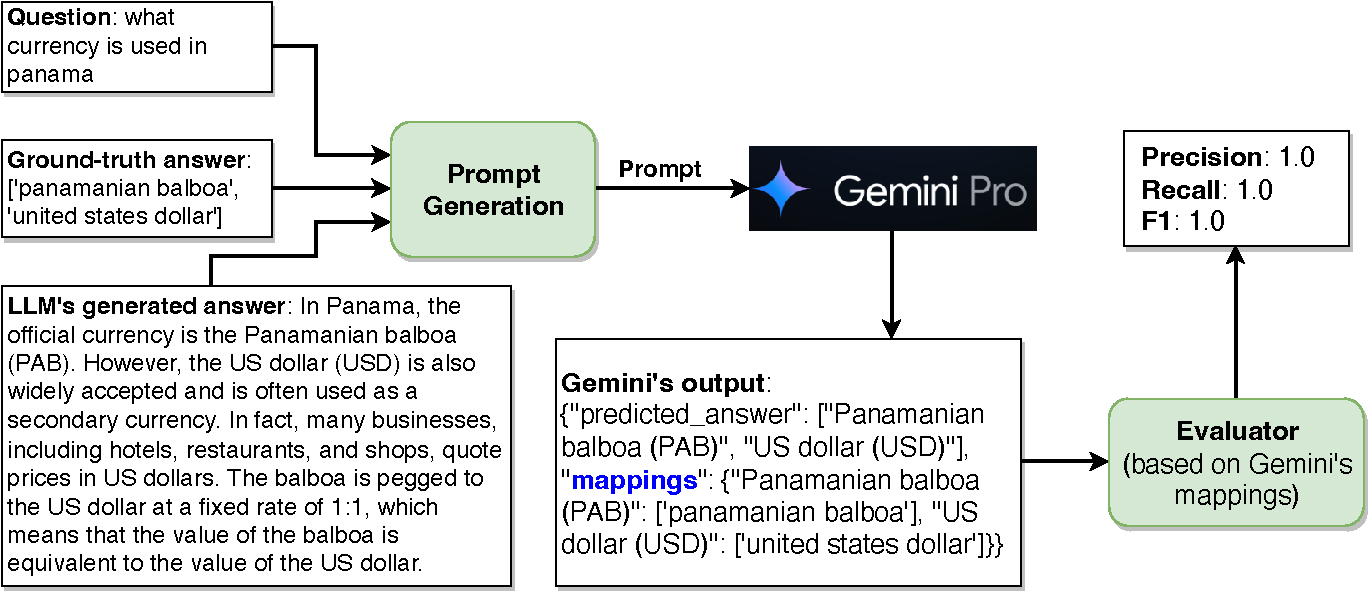
\includegraphics[width=.5\textwidth]{image/gemini_eval.pdf}
    \caption{LLM-based KBQA evaluation workflow using prompts for precision, recall, and F1 scores with Gemini-1.0-Pro as evaluator.}
    %\caption{LLM-based KBQA Evaluation Workflow. Given the input of \textit{question}, \textit{ground-truth answer}, and \textit{LLM's generated answer}, we create a prompt to extract answer-items and map them to ground-truth answer-items. Then, we calculate the precision, recall, and F1 based on the mappings of generated and ground-truth answer-items. We use Gemini-1.0-Pro for this evaluation task.} %The generated answer is taken from Llama 3-8B. }
    \label{fig:gemini_eval}
\end{figure}

% In KBQA task, the most common type of answer is a list of entities from the KG. For example, the answer to the question ``What language is spoken in Switzerland?'' is ``[Italian language, German language, French, Romansh language]''. While we can request LLMs to generate answers in the format of a list of entities, not all LLMs consistently follow this output format request. Therefore, it is crucial to process the answers returned by LLMs to extract the entity list for evaluation. One solution is to use Named Entity Recognition (NER); however, answers can contain other types of information besides named entities. Additionally, the wording used in answers might differ from the KG's entities even though they refer to the same entity, such as ``United States Dollar'' versus ``US dollar (USD)''.

% To resolve this problem, we propose an LLM-based evaluation method where an LLM is requested to extract answer-items (entities) from the generated answer and map them to the ground-truth answer-items. Figure \ref{fig:gemini_eval} shows the LLM-based KBQA evaluation workflow with an actual example using an answer generated from Llama 3-8B. We first construct a prompt using our pre-defined prompt template, shown in Listing \ref{list:gemini_prompt}. The prompt contains the input question, ground-truth answer, LLM's generated answer, and a request to extract answer-items and map them to the ground-truth answer-items. As shown in Figure \ref{fig:gemini_eval}, Gemini outputs a list of \textit{predicted answers} and a \textit{mapping} which maps each item in the predicted answers with those in ground-truth answers. Noted that one predicted answer-item can be mapped to more than one ground-truth answer-item or none (i.e., wrong answer). 

In the KBQA task, answers are typically lists of entities from the KG. For instance, the answer to ``What language is spoken in Switzerland?'' is ``[Italian, German, French, Romansh]''. While LLMs can be asked to generate entity lists, they do not always follow this format. Therefore, processing LLM-generated answers to extract entity lists for evaluation is crucial. Using Named Entity Recognition (NER) alone is not sufficient because answers may include non-entity information and differing entity wordings, e.g., ``United States Dollar'' versus ``US dollar (USD)''.
To address this, we propose an LLM-based evaluation method where an LLM extracts and maps answer-items (entities) from the generated answer to the ground-truth entities. Figure \ref{fig:gemini_eval} illustrates this workflow with an example generated by Llama-3-8B. We construct a prompt using a predefined template (Listing \ref{list:gemini_prompt}), including the question, ground-truth answer, LLM-generated answer, and a request for entity extraction and mapping. As shown in the figure, Gemini outputs a list of \textit{predicted answers} and a \textit{mapping} of predicted answers to ground-truth answers. A predicted answer can map to multiple ground-truth items or none (i.e., incorrect answer).

The mapping is then used to compute evaluation metrics including Precision, Recall, and F1. The details are as follows. 
Given a question, we denote the ground-truth answer as $A=[A_1, A_2, \cdots, A_n]$ and the list of predicted answer-items as $\hat{A}=[\hat{A}_1, \hat{A}_2,\cdots, \hat{A}_m]$. The mapping is denoted as $M=\{\hat{A}_1: M_1, \hat{A}_2: M_2, \cdots, \hat{A}_m: M_m\}$ where $M_i$ is a list of ground-truth answer-items matched with the corresponding predicted answer-item, i.e., $M_i \subseteq A$ ($i=1, \cdots, m$) and $M_i$ is empty when the predicted answer-item is wrong. A predicted answer-item is called \textit{correct} if it matches with at least one of the ground-truth answer-items.
We define $c_G=|\text{set}(M_1\cup M2 \cup \cdots \cup M_m)|$ as the number unique ground-truth answer-items that matched with at least one predicted answer-item and $c_P$ as the number of correct predicted answer-items. The final number of correct answers is chosen as the smallest number between $c_G$ and $c_P$. 
% :
% \begin{align}
%     c = \left\{\begin{matrix}
% c_G & \text{if } c_G < c_P\\ 
% c_P & \text{otherwise} 
% \end{matrix}\right.
% \end{align}
This is to deal with the cases where different predicted answer-items carry the same meaning (mapped to the same ground-truth answer-item). The precision and recall are then computed as $\frac{c}{|\hat{A}|}$ and $\frac{c}{|A|}$, respectively. 
% follows: 
% \begin{align}
%     \text{precision} = \frac{c}{|\hat{A}|}
% \end{align}
% \begin{align}
%     \text{recall} = \frac{c}{|A|}
% \end{align}
F1 score is computed as the harmonic mean of precision and recall. 
We chose \gemini for this evaluation task because of its strong natural language processing capabilities and its availability during our experiments.

\subsection{Tuning RPP for All Models and Datasets}
\label{sec:gain_all}
\begin{figure}[ht]
    \centering
    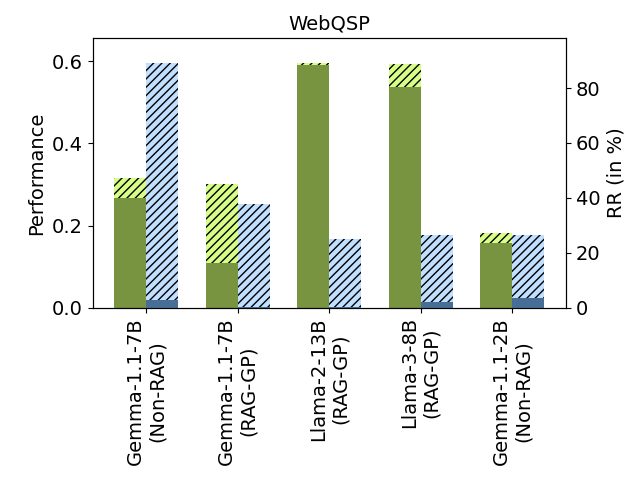
\includegraphics[width=1\linewidth]{image/chart_00_selected_wd.png}
    \caption{Top-5 model with highest RR reduction for \webqsp dataset}
    \label{fig:chart_00_selected_wd}
\end{figure}
\begin{figure}[ht]
    \centering
    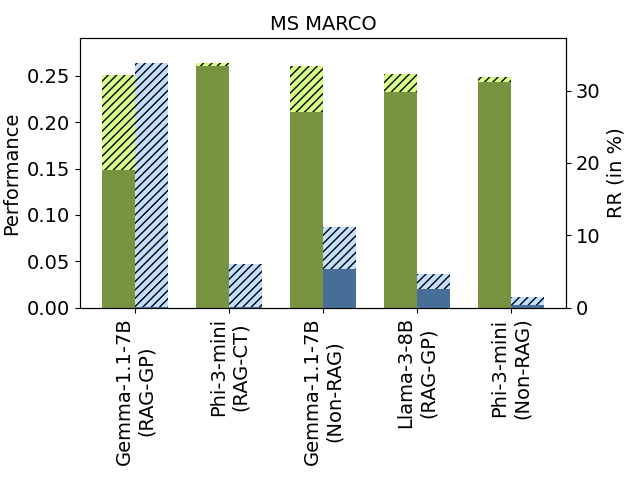
\includegraphics[width=1\linewidth]{image/chart_00_selected_mm.png}
    \caption{Top-5 model with highest RR reduction for \ms dataset}
    \label{fig:chart_00_selected_mm}
\end{figure}
\begin{figure}[ht]
    \centering
    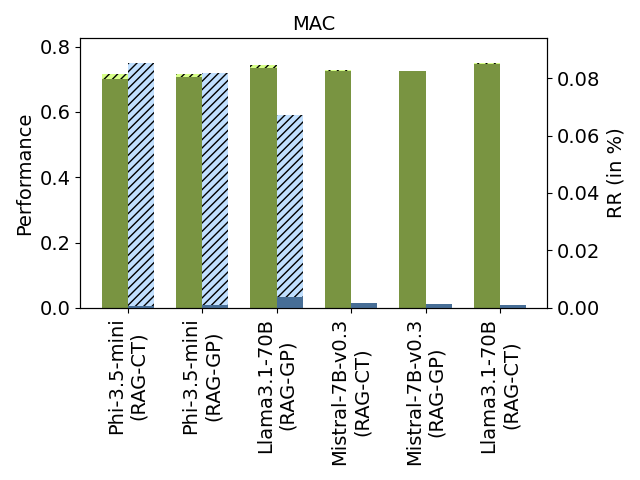
\includegraphics[width=1\linewidth]{image/chart_00_selected_mac.png}
    \caption{Tuning RPP of all models for \mac dataset}
    \label{fig:chart_00_selected_mac}
\end{figure}

We visualize the best performance when tuning RPP using original evaluation metrics (Original) and our proposed repetition-aware performance metric (RAP). RAP helps find RPP values that minimally reduce performance while significantly lowering repetition ratio (RR). Results for all models across three datasets are shown in Figure \ref{fig:chart_00_specific} (\webqsp, \ms) and \ref{fig:chart_00_selected_mac} (\mac). Figure \ref{fig:chart_00_selected_wd} and \ref{fig:chart_00_selected_mm} show the top-5 highest RR reduction after tuning for \webqsp and \ms dataset respectively. Green color bar indicates performance and blue color bar indicates RR. The hatched bar visualize the magnitude of reduction after tuning. 

\subsection{How Severe can Repetition be for Other Models and Datasets?}
\label{sec:how_severe}
Figure \ref{fig:webqsp_top3} visualize the top-3 highest and lowest RR for WebQSP, while Figure \ref{fig:chart_02_wd_all}, \ref{fig:chart_02_mm_all}, and \ref{fig:chart_02_mac_all} visualize all models for \webqsp, \ms, \mac respectively. The leftmost three models show the Top-3 highest RR, while the rightmost three display the lowest. The ratio of repeated text length to text length is also visualized. Colored squares above each point indicate the percentage of repeated questions, with blue, yellow, and red squares marking values below 10\%, between 10-20\%, and above 20\% respectively. The x-label indicates the model, the prompting method, and the RP of the RR. 
\begin{figure}[t]
    \centering
    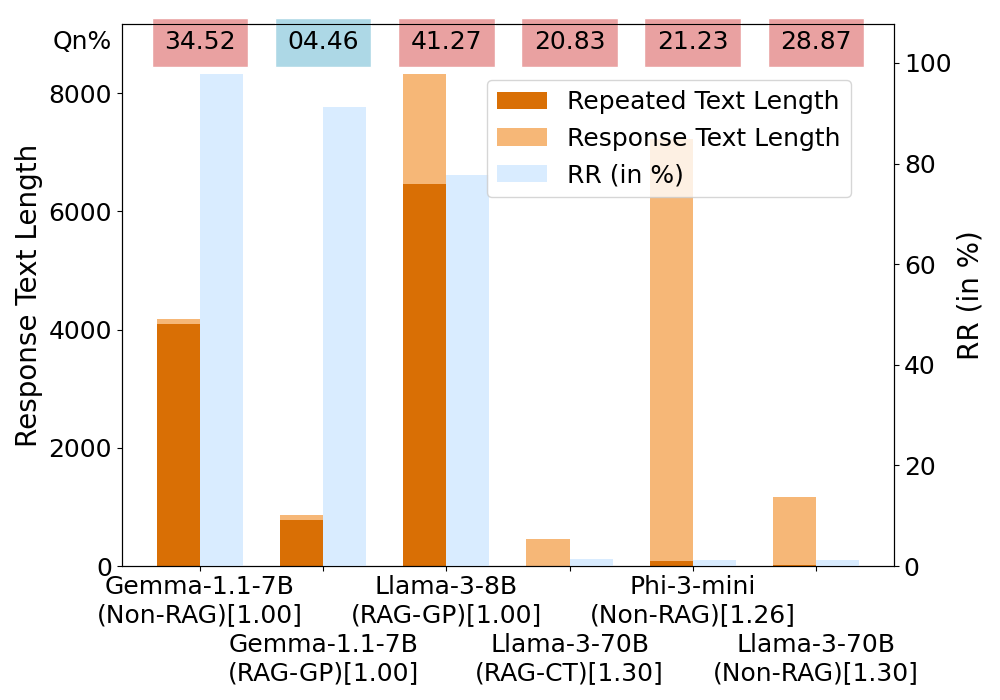
\includegraphics[width=1\linewidth]{image/chart_02_wd.png}
    \caption{Top-3 highest and lowest RR for \webqsp dataset}
    \label{fig:webqsp_top3}
\end{figure}
\begin{figure}[t]
    \centering
    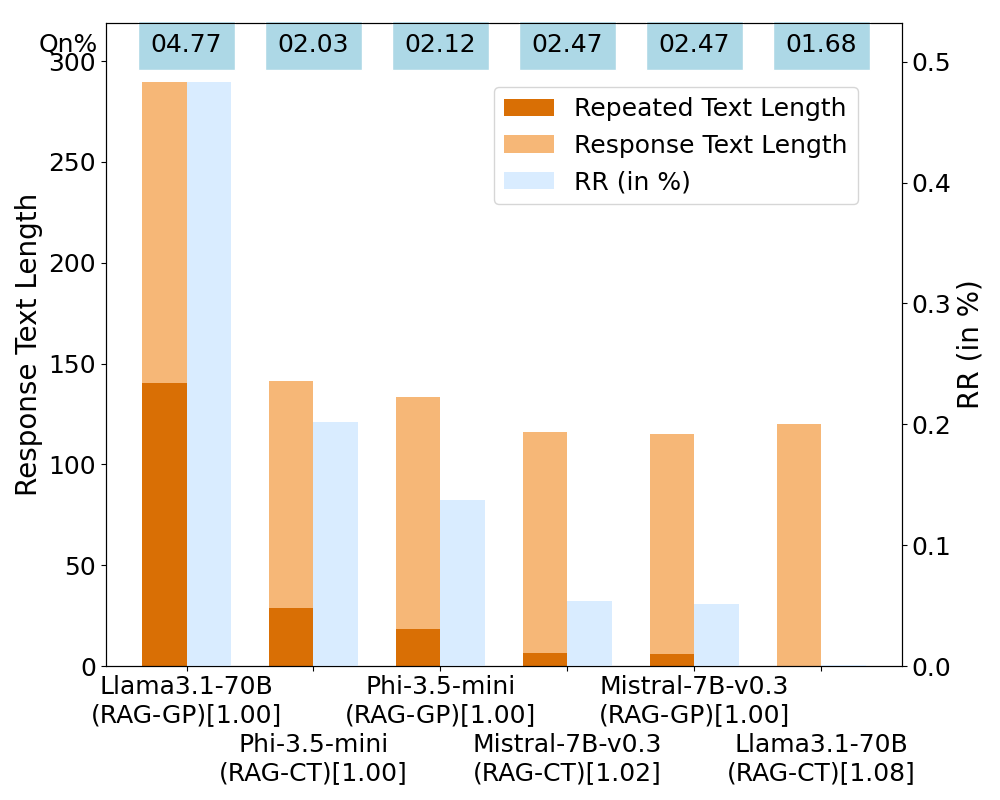
\includegraphics[width=1\linewidth]{image/chart_02_mac_all.png}
    \caption{Percentage of repeated responses, repeated text length, and RR for \mac dataset}
    \label{fig:chart_02_mac_all}
\end{figure}
\begin{figure*}[t]
    \centering
    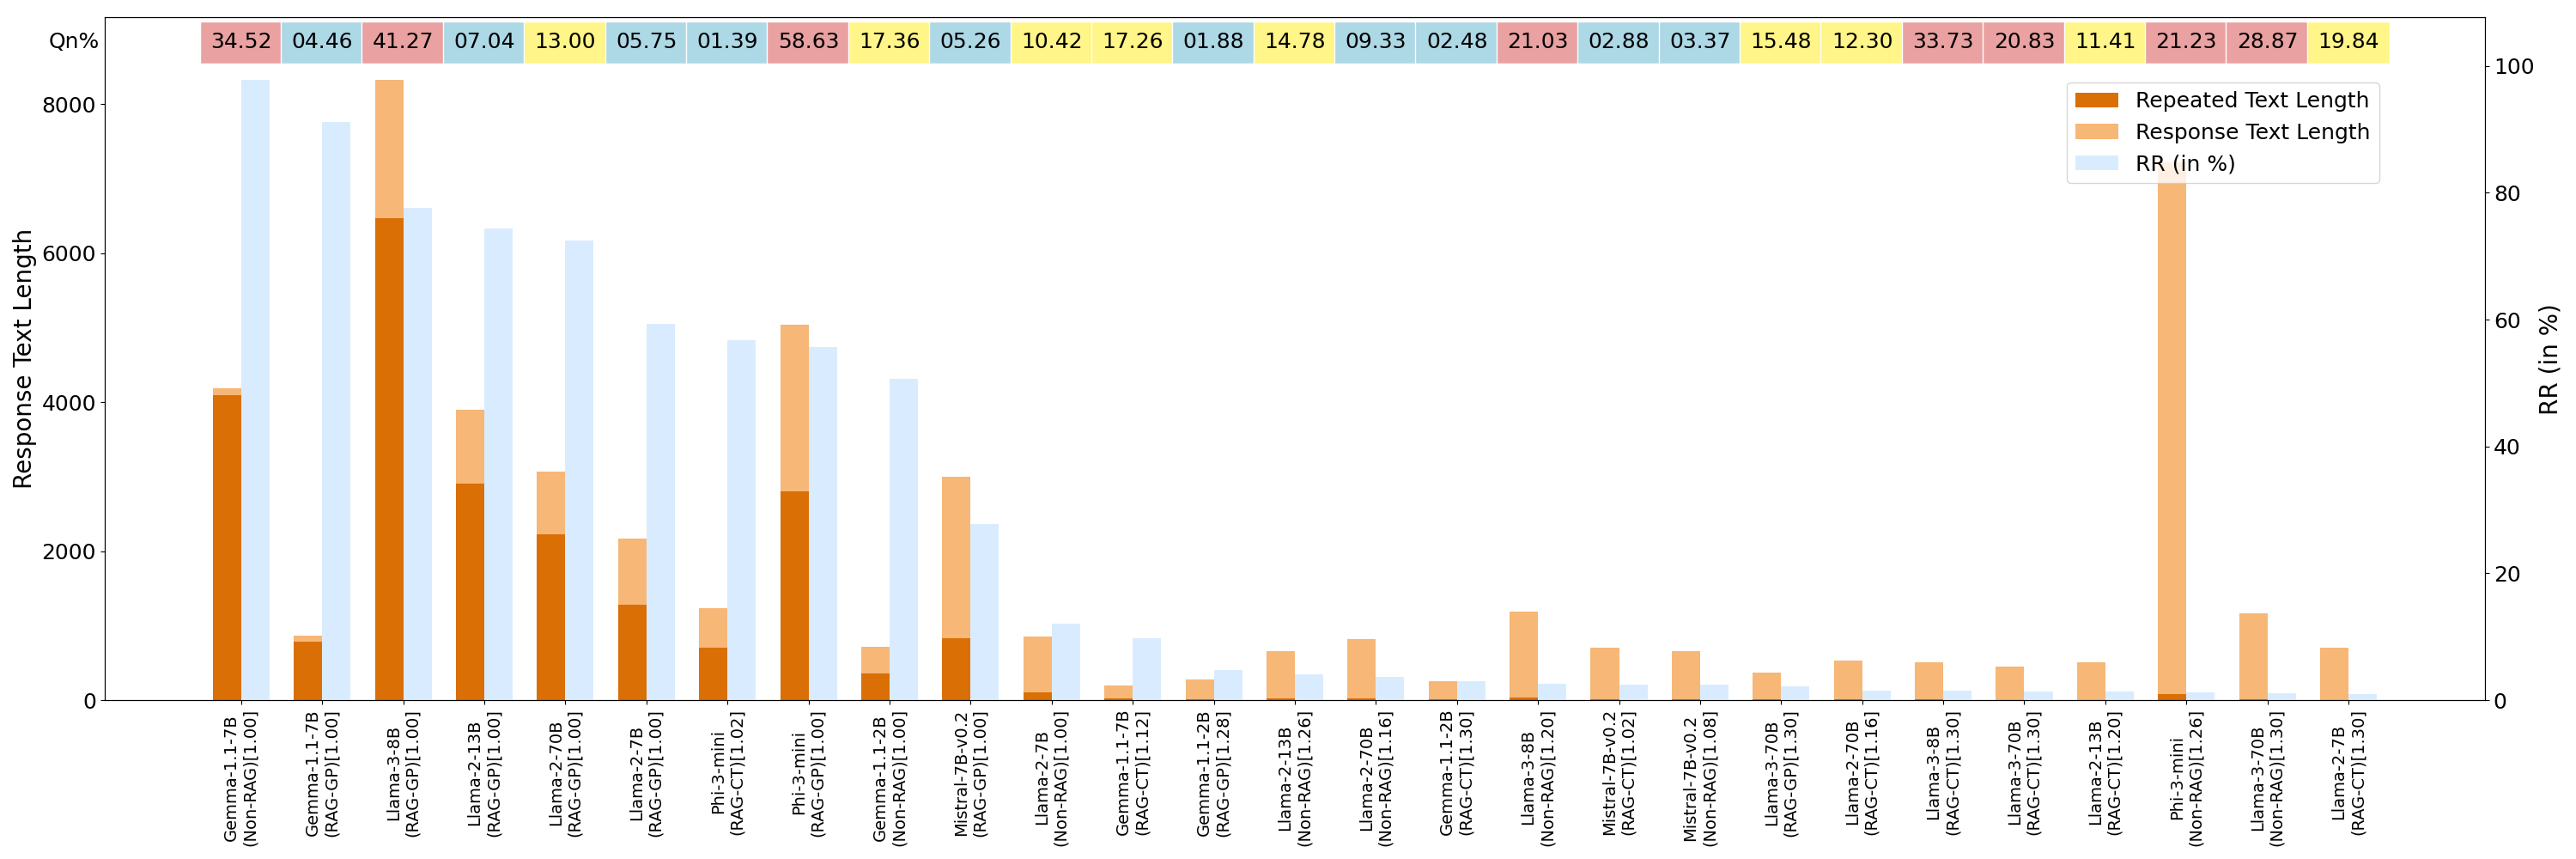
\includegraphics[width=\textwidth]{image/chart_02_wd_all.png}
    \caption{Percentage of repeated responses, repeated text length, and RR for \webqsp dataset}
    \label{fig:chart_02_wd_all}
\end{figure*}
\begin{figure*}[t]
    \centering
    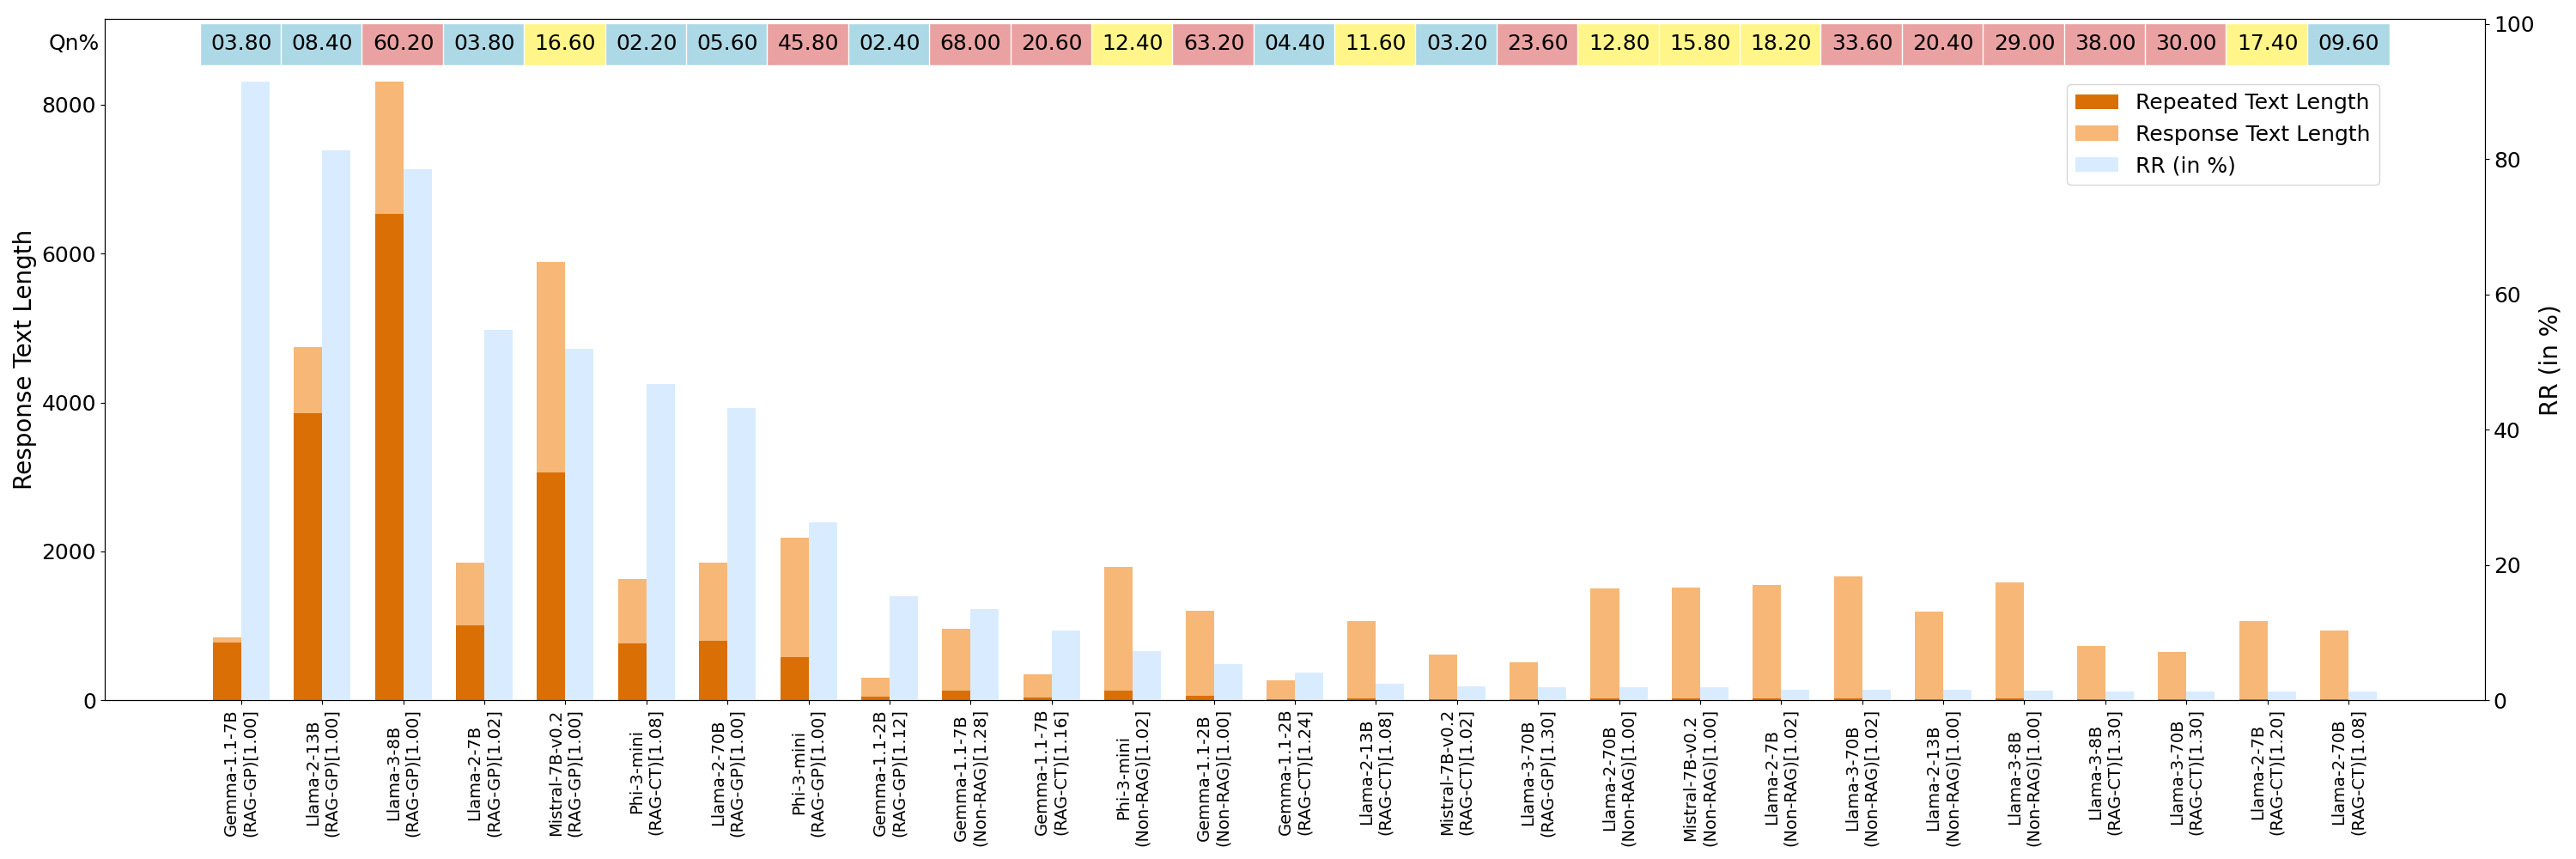
\includegraphics[width=\textwidth]{image/chart_02_mm_all.png}
    \caption{Percentage of repeated responses, repeated text length, and RR for \ms dataset}
    \label{fig:chart_02_mm_all}
\end{figure*}
\begin{figure*}[t]
    \centering
    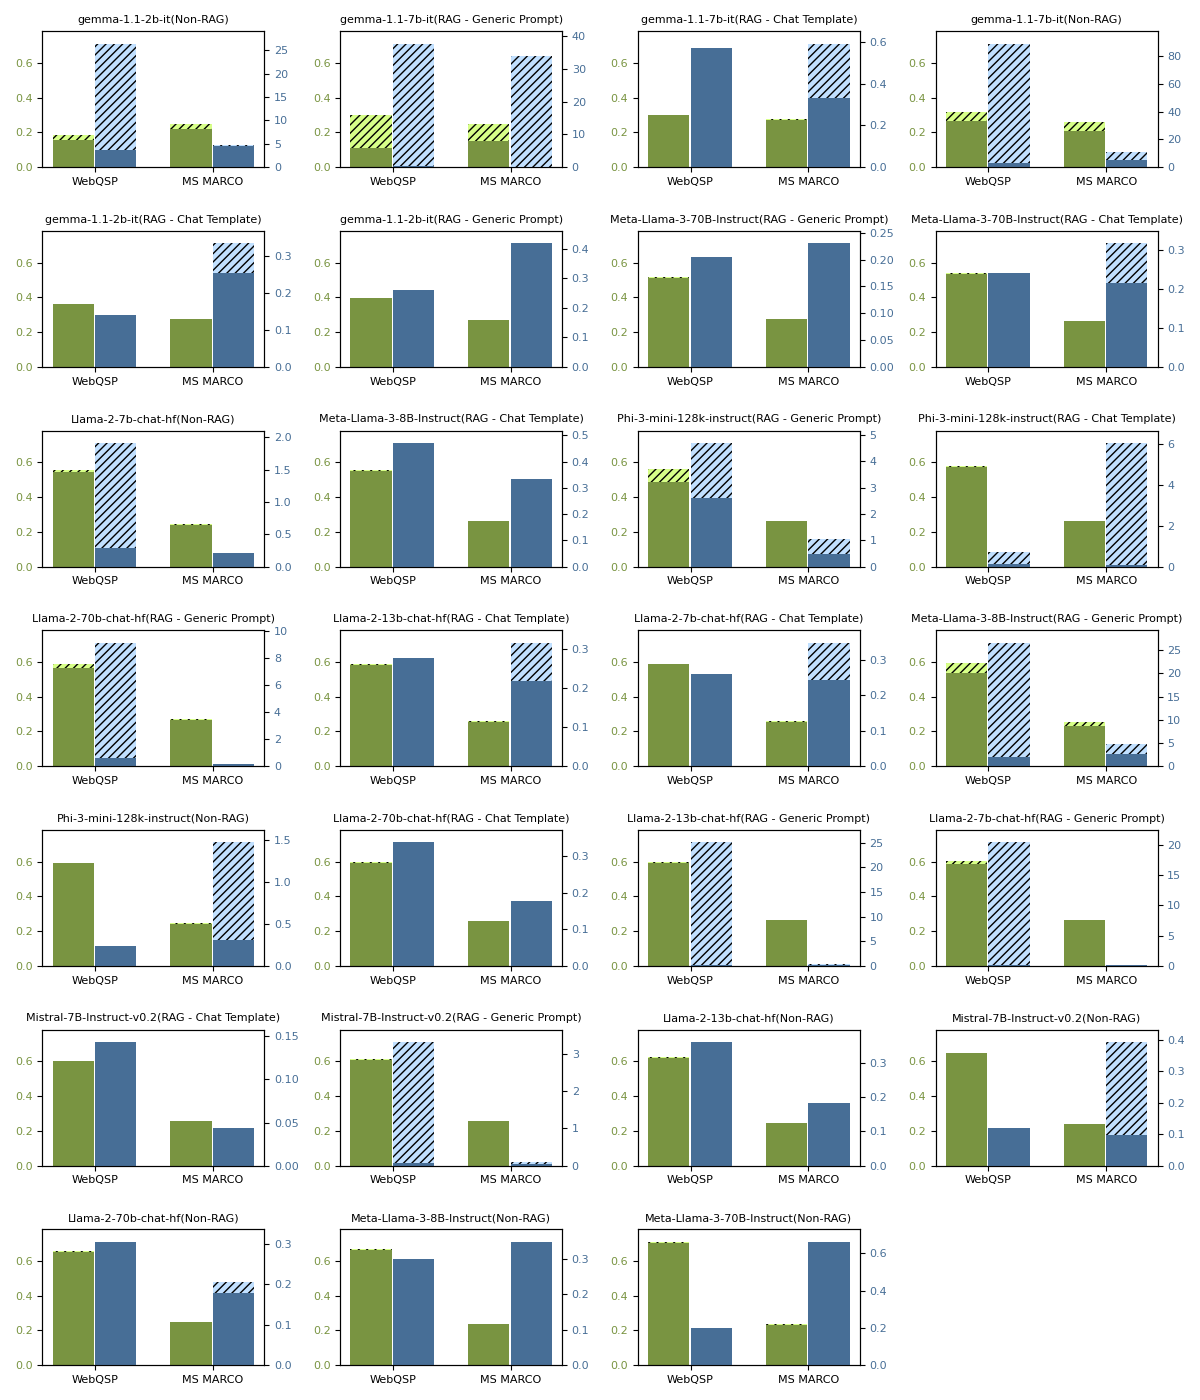
\includegraphics[width=\textwidth]{image/chart_00_specific.png}
    \caption{Tuning RPP of all models for \webqsp and \ms dataset}
    \label{fig:chart_00_specific}
\end{figure*}



\section{Experiments}
% \subsection{Impact of RPP on Repetition + Performance}

% \subsection{RAP enable tuning to obtain the trade-off between performance and repetition
% }

% \subsection{Compare the performance using tuned RPP (based on RAP)
% }

% \subsection{Further Discussions}

\subsection{Experimental settings}
\textbf{Datasets.} 
% \begin{table}[]
% \centering
% \caption{Datasets used in our experiments. The Size refers to the number of questions or samples in the test set. }
% \label{tab:dataset}
% \begin{tabular}{l|l|r}
% \toprule
% Dataset                & Task                & \multicolumn{1}{l}{Size} \\ \midrule
% \webqsp  & Knowledge Base QA   & 1008                     \\
% \ms     & Open-ended QA       & 500                      \\
% \mac    & Machine Translation & 1133                    \\ \bottomrule
% \end{tabular}
% \end{table}
We conduct the experiments using three datasets including \webqsp \cite{yih2016value} and \ms
% \footnote{\url{https://microsoft.github.io/msmarco/}}
\cite{bajaj2016ms, huang2024performance} for question answering (QA), and \mac \cite{huang2025optimizing} for Chinese-English machine translation (MT). The datasets contain 1,008, 500, and 1,133 testing questions, respectively. To perform RAG on \webqsp, we crawled relevant articles from Wikipedia, and retrieve 8 most relevant document chunks when answering each question for RAG prompting. We also adopt Gemini-1.0-Pro to evaluate for the knowledge base question answering task (KBQA) where the ground-truth answers contains lists of entities instead of natural language text. More details of the dataset and LLM-based KBQA evaluation are presented in the Appendix (\ref{sec:data}). 

% as detailed in Section \ref{sub:data-col-pre}.

% \noindent
% \textbf{Open-source LLMs.} We evaluate nine open-source LLMs including Llama-2 (7B, 13B, 70B), Llama-3 (8B, 70B), Gemma-1.1 (2B, 7B), Phi-3-mini (3.8B), and Mistral-7B. These are currently some of the most popular open-source LLMs suitable for use in commercial applications (permitted by their licenses).
% \textbf{Open-source LLMs.} \new{
% \new{Table \ref{tab:ai_models} provides an overview of all the models utilized in our study, detailing their companies, model names, and corresponding HuggingFace model identifiers. 
% For QA tasks, we evaluate nine open-source LLMs, including Llama-2 (7B, 13B, 70B), Llama-3 (8B, 70B), Gemma-1.1 (2B, 7B), Phi-3-mini (3.8B), and Mistral-7B. For MT task, we evaluate three open-source LLMs: Phi-3.5-mini (3.8B), Mistral-7B, and Llama-3.1-70B. These models are among the most popular open-source LLMs suitable for use in commercial applications, as permitted by their respective licenses. More details can be found in the Appendix (\ref{subsec:overview_llms}). %\ref{subsec:overview_llms}.
% }
\textbf{Open-Source LLMs.} This study evaluates a diverse set of open-source large language models (LLMs) for question answering (QA) and machine translation (MT) tasks. For QA, we assess nine models: Llama-2 (7B, 13B, 70B), Llama-3 (8B, 70B), Gemma-1.1 (2B, 7B), Phi-3-mini (3.8B), and Mistral-7B. For MT, we evaluate three models: Phi-3.5-mini (3.8B), Mistral-7B, and Llama-3.1-70B.

Table~\ref{tab:ai_models} provides an overview of these models, including their respective companies, model names, Hugging Face identifiers, and the tasks they were evaluated on. This selection spans a broad range of model sizes and architectures, representing the state of the art in open-source LLM development. These models are widely used in commercial applications under their respective licenses.

The diversity of this selection enables a robust comparison across model families and sizes, offering insights into the relative strengths of different open-source LLMs in QA and MT tasks.

\begin{table*}[htbp]
\caption{Overview of Large Language Models and Their Specifications by Task}
\label{tab:ai_models}
\centering
\resizebox{.8\textwidth}{!}{
\begin{tabular}{l|l|l|l}
\toprule
\textbf{Company} & \textbf{Model Name} & \textbf{Hugging Face Model ID} & \textbf{Task} \\
\midrule
\multirow{6}{*}{Meta} 
& Llama-2-7B & meta-llama/Llama-2-7b-chat & QA \\
& Llama-2-13B & meta-llama/Llama-2-13b-chat & QA \\
& Llama-2-70B & meta-llama/Llama-2-70b-chat & QA \\
& Llama-3-8B & meta-llama/Meta-Llama-3-8B-Instruct & QA \\
& Llama-3-70B & meta-llama/Meta-Llama-3-70B-Instruct & QA \\
& Llama-3.1-70B & shenzhi-wang/Llama3.1-70B-Chinese-Chat & MT \\
\midrule
\multirow{2}{*}{Microsoft} 
& Phi-3-mini & microsoft/Phi-3-mini-128k-instruct & QA \\
& Phi-3.5-mini & microsoft/Phi-3.5-mini-instruct & MT \\
\midrule
\multirow{2}{*}{Google} 
& Gemma-1.1-2B & google/gemma-1.1-2b-it & QA \\
& Gemma-1.1-7B & google/gemma-1.1-7b-it & QA \\
\midrule
\multirow{2}{*}{Mistral AI} 
& Mistral-7B-v0.2 & mistralai/Mistral-7B-Instruct-v0.2 & QA \\
& Mistral-7B-v0.3 & shenzhi-wang/Mistral-7B-v0.3-Chinese-Chat & MT \\
\bottomrule
\end{tabular}
}
\end{table*}

\textbf{Automating QA and MT Tasks with LLMs.} 
We developed a Python script specifically designed to evaluate the performance of LLMs on QA and MT tasks. The script leveraged the open-source HuggingFace Transformers library~\cite{wolf2020transformers} and was executed across all models and datasets. For QA tasks, an RPP range of 1.0 to 1.3 was applied, while for MT tasks, an RPP range of 1.0 to 1.1 was used, both with increments of 0.02. To ensure consistency and reproducibility across experiments, the temperature was set to 0 and \texttt{top\_p} was fixed at 0.95.
% \noindent
% \textbf{Automated Question Answering with LLMs:} 
% \textbf{\new{Automated Answer Generation with LLMs:}} 
% \new{We developed Python scripts to automate interactions with LLMs for generating answers. The scripts were applied to all models and datasets, with the \rp ranging from 1.0 to 1.1 for MT task and up to 1.3 for QA tasks, incremented by 0.02.}
% We developed a Python script leveraging LangChain and HuggingFace Transformers\footnote{\url{https://huggingface.co/docs/transformers/en/index}} to automate interactions with LLMs for generating answers to questions in the datasets. The script was executed using all models and both datasets, with a repetition penalty ranging from 1.0 to 1.3 in increments of 0.02. 
% We developed a Python script to automate interactions with LLMs for generating answers. The script was run on all models and datasets, applying \rp ranging from 1.0 to 1.3 in 0.02 increments.

% The questions and generated answers, along with other data elements from the datasets, were stored in CSV files for further data processing, such as detecting repetitions and evaluating performance.

% \noindent
\textbf{Prompt Templates:} 
To investigate LLMs’ behaviors under different prompting strategies, we implemented three QA prompt templates: (1) \textit{RAG - Generic Prompt} (\raggen): a uniform basic template for all models; (2) \textit{RAG - Chat Template} (\ragtem): LangChain’s default template tailored to each LLM’s chat format, maintaining the same core content; and (3) \textit{Non-RAG}: simulates a single-turn conversation in the LLM’s chat format.
For MT, we used two templates: (1) \textit{MT - Generic Prompt} (\mtgen): a basic template applied uniformly, and (2) \textit{MT - Chat Template} (\mttem): a template designed for each LLM’s chat format. Prompt templates are shown in the Appendix (\ref{sec:prompt}). 

% To investigate LLMs’ behaviors under different prompting strategies, we implemented three prompt templates \new{for QA}: (1) \textit{RAG - Generic Prompt} (\raggen): using the same basic prompt template for all the models.
% (2) \textit{RAG - Chat Template} (\ragtem): using LangChain’s default template to match each LLM’s chat format. While the template varies across model families, the main message content remains the same. 
% (3) \textit{Non-RAG}: simulates a single-turn conversation between a human and the LLM, following the LLM’s chat format. 
% \new{For MT, we implemented two prompt templates: 
% (1) \textit{MT - Generic Prompt} (\mtgen): a basic prompt template applied uniformly across all models, and 
% (2) \textit{MT - Chat Template} (\mttem): using the template to fit each LLM’s chat format.} 
%
% The prompt templates for Llama-3 models is shown in the Appendix. 

% The Non-RAG prompt for Llama-3 models is shown in Listing \ref{list:non-rag} in Appendix.

% \noindent
\textbf{Evaluation Metrics:} For \webqsp, we use \textit{precision}, \textit{recall}, and \textit{F1} scores. For \mds, \new{we employ BERTScore~\cite{zhang2019bertscore}, using deberta-xlarge-mnli model to ensure optimal performance, as it provides the highest correlation with human evaluations. Results are reported as the average F1 score across the entire dataset, referred to as \textit{BERT-F1}. 
For \mac, we employ the Crosslingual Optimized Metric for Evaluation of Translation (\textit{COMET}), a neural-based evaluation metric that leverages contextual embeddings from pretrained language models to assess translation quality~\cite{rei2022comet}. COMET has demonstrated strong correlation with human judgments, making it a reliable metric for translation evaluation.}
%we use ROUGE-L~\cite{lin2004rouge,joshi2023deepsumm} and BLEU-1~\cite{dey2022evaluating} to assess answer quality. 
%
For repetition evaluation, we report the repetition ratio (Equation \ref{eq:rr_dataset}).
%We also introduce an overall performance score, denoted as \hm and calculated as the harmonic mean of BLEU-1 and ROUGE-L.
% : 
% \begin{align}
%     H = \frac{2 \times \text{BLEU-1} \times \text{ROUGE-L}}{\text{BLEU-1} + \text{ROUGE-L}} 
% \end{align}
We also report the \rap scores, applied on the corresponding evaluation metrics (Section \ref{sec:rap}).

% Existing metrics: What metrics for WebQSP, What metrics for MS Macro. 
% NEW: Repetition Factor
% NEW: Repetition Factor Adjusted Perf Scores



% \begin{itemize}
%     \item Investigate the impact of \rp on repetition and performance 
%     \item \rf to incorporate repetition penalty in the performance so that we can perform hyperparamter tuning 
    
% \end{itemize}


% \noindent
% \textbf{Repetition Detection - Baseline Method} 
% To benchmark our proposed repetition detection method, we develop a baseline method based on \cite{Fu2020ATA} that identifies adjacent identical word phrases using a suffix array \cite{10.5555/320176.320218} sorted lexicographically. The method scans the suffix array in multiple passes, comparing row-adjacent phrases to find exact matches where their index distance equals the phrase length. A greedy approach is then used to extract the longest combination of adjacent repeated phrases. See Appendix for more details.
% To benchmark our proposed repetition detection method, we develop a baseline method based on \cite{Fu2020ATA} to identify adjacent identical word phrases. To simulate this, tokenized words of the input text are stored in a suffix array \cite{10.5555/320176.320218}, which is sorted lexicographically. 
% For example, "This is repeated is repeated text" has 6 suffixes (Figure \ref{fig:suffix_array_simulation}) stored as indexes 1, 3, 2, 4, 5, 0. 
% To find repeated phrases, the method scans the suffix array in $N$ passes, where $N$ equals the size of tokenized words, comparing row-adjacent phrases of length 1 ... $N$. Phrases are considered repeating if they match exactly and their suffix array index distance equals the phrase length. A greedy approach is then used to extract the longest combination of adjacent repeated phrases. 
% An experimental result demonstrate that \alg is faster by 12\% compared to the baseline method and performs comparably better than the baseline algorithm. Moreover, the method discovers abnormalities in the text that were not addressed by the baseline method, details of which will be provided in section \ref{subsec:evaluating-text-abnormalities}. 



% \textbf{Findings}
% \begin{enumerate}
%     \item Chat template significantly reduce repetition. It's not well-known/common practice by developers to use Chat template, in LLM application development. 
%     \item For generic prompt, increasing RPP normally reduce repetition. With Chat template model, the impact of \rpp is not as effective, for some model, increasing too high RPP can lead to higher repetition 
%     \item We show that RPP also have impact on the performance, so a balance approach can be achieved with RAP (with minimal findings)
% \end{enumerate}

% \textbf{Experiments}
% \begin{enumerate}
%     \item Impact of RPP on Repetition and Performance: showing results of all models, all datasets, all prompts. (@Donghao)
%     \item Optimizing the trade-off between performance and repetition. Objective is to show how to tune \rpp using RAP. (Existing content, maybe shorten). Remove numbers, change MTR to RR. Add for MT (@Donghao) 
%     \item comparing the best original + \rap of all models. The figures combining of figure-1-like figures. 
%     \item What is the percentages of responses having repetition, if having repetition, how severe it is? Choose few models and show the results. 
% \end{enumerate}



% \begin{align}
%     Gain = \frac{RR_{Origin} - RR_{RAP}}{P_{origin} - P_{RAP}}
% \end{align}

\subsection{Impact of \rpp on Repetition and Performance}
\label{subsec:impact_of_rpp}
\begin{figure*}[ht!]
    \centering
    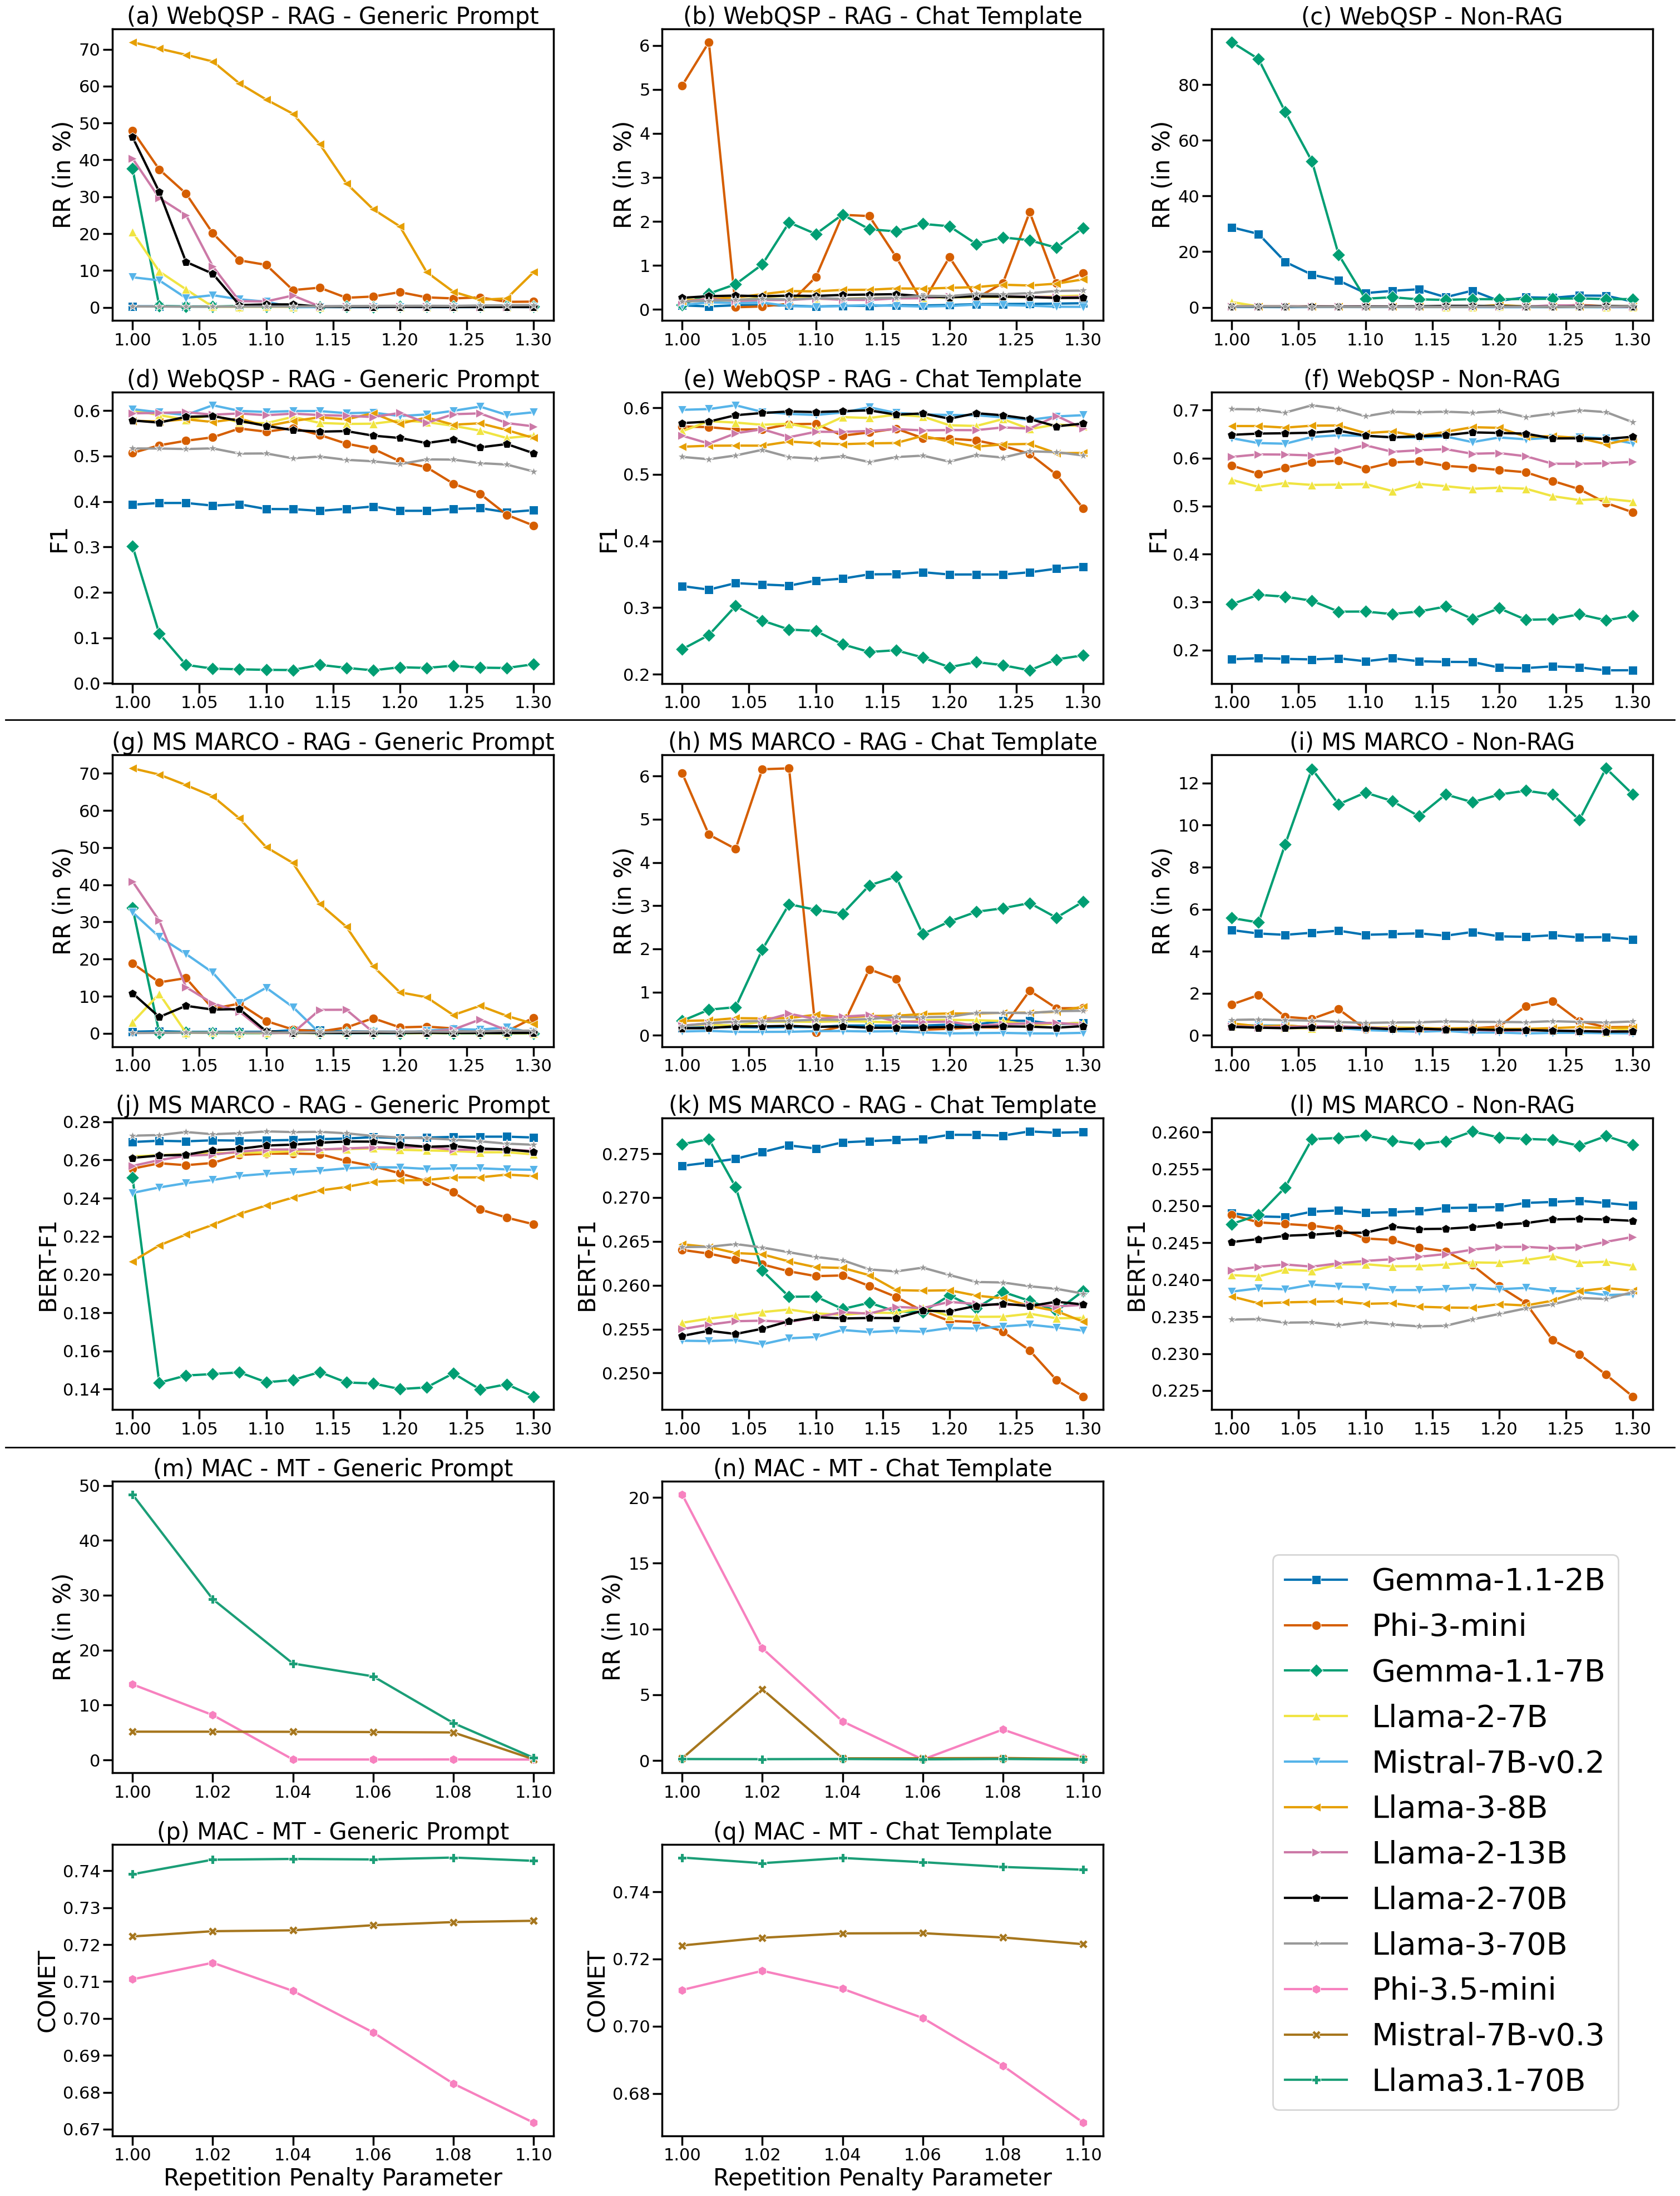
\includegraphics[width=\textwidth]{image/all-metrics-across-models_v2.png}
    \caption[Performance and Repetition Metrics Across Models]{
    Illustrating the impact of \rpp on \rr and performance across models, datasets, and prompting strategies. 
    % Results highlight the effectiveness of Chat Templates in reducing repetition while maintaining competitive performance, as well as the diminishing returns of increasing RPP beyond certain thresholds.
    % Performance and \rr when varying \rpp. This figure illustrates the impact of \rpp on repetition (RR) and performance (F1, BERT-F1, COMET) across different models, datasets (WebQSP, MS MARCO, MAC), and prompting strategies. Results highlight the effectiveness of Chat Templates in reducing repetition while maintaining competitive performance, as well as the diminishing returns of increasing RPP beyond certain thresholds.
    %\todo{to make subfigure title much bigger, can we draw a line between datasets?}
    }
    \label{fig:all-metrics-across-models_v2}
\end{figure*}

Figures \ref{fig:all-metrics-across-models_v2} illustrates the impact of \rpp on the repetition and performance of different open-source LLMs on the three datasets, using different prompting strategies. 
The results show that increasing RPP generally reduces repetition across strategies and datasets but often leads to a decline in performance. The trending and severity vary by model; for instance, while Phi-3-mini’s performance on MS MARCO-RAG-GP dropped significantly with RPP above 1.14, Llama-3-8B showed improved performance with higher RPP values under the same conditions. 
% The trade-off between reducing repetition and maintaining accuracy becomes evident beyond 1.15–1.20.
Therefore, selecting an optimal RPP value is crucial to balance repetition reduction with minimal impact on performance.
% metrics like F1, BERT-F1, or COMET.
%dataset

The datasets also show different behaviors. WebQSP generally exhibits higher repetition levels (e.g., at RPP = 1.0) than MS MARCO, especially with the RAG-GP strategy. This indicates that the nature of the dataset and task also influence repetition tendencies. In MAC dataset, despite a smaller RPP range tested, repetition still decreases as RPP increases. For both QA datasets, the Chat Template strategy consistently reduces repetition, showing lower RR values than the Generic Prompt approach. This suggests that the Chat Template effectively minimizes repetition in QA tasks. However, it surprisingly does not offer the same benefit for MT task, where increasing RPP effectively reduces repetition.



% Unlike QA tasks, the Chat Template and Generic Prompt strategies show similar repetition levels in MT.

% Chat template 
% Impact of RPP 
% , but Llama-3-8B in the same setting gets higher performance with higher value of RPP. 

% Several key insights can be drawn from these results:

% \noindent 
% \textbf{Chat Template Superiority}: 
% Across both QA datasets and all RPP values, the Chat Template strategy consistently achieves the lowest levels of repetition. This is reflected in lower RR values compared to the Generic Prompt approach. These results suggest that using a Chat Template is an effective method for minimizing repetitive content in model outputs for QA task. Supperisingly, using template does not seem to help for machine translation, although repetition can be reduced easily by increasing \rpp for this task. 

% \noindent 
% \textbf{The impact of RPP}: the results show that increasing RPP generally reduces repetition across different strategies and datasets. 
% However, it is also shown that using higher RPP value often leads to a decline in performance for most of the models and settings. The severity of the impact varies depending on the model. For example, Phi-3-mini's performance in MS MARCO-RAG-Generic Prompt significantly reduced when using RPP higher than 1.14.
% The impact is particularly noticeable as RPP increases beyond 1.15--1.20, where the trade-off between reducing repetition and maintaining model accuracy becomes evident. Therefore, it is important to choose an optimal RPP value that balances the reduction in repetition with minimal impact on performance (F1, BERT-F1, or COMET).
% \noindent \textbf{Diminishing Returns}: For most strategies, the reduction in repetition plateaus as RPP increases beyond certain thresholds (typically around 1.20--1.25). This indicates that there may be an optimal range for RPP settings, beyond which further increases provide minimal additional benefits in terms of repetition reduction. 

% \noindent \textbf{Dataset Differences}: The behaviors are also different in the different datasets. WebQSP dataset generally exhibits higher baseline repetition levels (at RPP = 1.0) compared to MS MARCO, particularly for the RAG - Generic Prompt strategy. This indicates that the nature of the dataset and task can significantly influence repetition tendencies. In the MAC machine translation (MT) task, although a smaller range of RPP values was tested, repetition reduction is still evident as RPP increases. Interestingly, unlike the QA tasks, the Chat Template and Generic Prompt strategies show comparable levels of repetition in the MT task.

% These findings highlight the importance of carefully tuning the RPP and selecting appropriate prompting strategies to optimize model performance while minimizing undesirable repetition. The results also underscore the effectiveness of Chat Templates in managing repetition across different models and datasets.

% Figure \ref{fig:mean-metrics-across-models} shows the results of average mean total repetitions and performance when varying \rp.  


% \textbf{Mean Total Repetitions:} Increasing RPP generally reduces mean total repetitions across all models and prompt templates, indicating that a higher RPP effectively suppresses repetitive content. The \raggen exhibits the highest repetition issues, with mean total repetitions exceeding 600 at an RPP of 1.0, gradually decreasing as RPP increases. Repetition issues generally cease when RPP is greater than or equal to 1.2, a trend consistent across other prompt templates.

% \textbf{Performance Metrics}: For the WebQSP dataset (Figures \ref{fig:mean-metrics-across-models}a and \ref{fig:mean-metrics-across-models}c), increasing RPP stabilizes or slightly reduces F1 scores for \raggen and \ragtem, while Non-RAG methods maintain relatively stable F1 scores. For the MS MARCO dataset (Figures \ref{fig:mean-metrics-across-models}b and \ref{fig:mean-metrics-across-models}d), overall performance declines with increasing RPP for \raggen and \ragtem, while Non-RAG methods remain stable.




% \textbf{Mean Total Repetitions:} Increasing RPP generally reduces mean total repetitions across all models and prompt templates, indicating that a higher RPP effectively suppresses repetitive content. The \raggen exhibits the highest repetition issues, with mean total repetitions exceeding 600 at an RPP of 1.0, gradually decreasing as RPP increases. Repetition issues generally cease when RPP is greater than or equal to 1.2, a trend consistent across other prompt templates.

% \textbf{Performance Metrics:} For the WebQSP dataset (Figures \ref{fig:mean-metrics-across-models}a and \ref{fig:mean-metrics-across-models}c), increasing RPP tends to stabilize or slightly reduce F1 scores for \raggen and \ragtem. Non-RAG methods maintain relatively stable F1 scores across different RPP values. Conversely, for the MS MARCO dataset (Figures \ref{fig:mean-metrics-across-models}b and \ref{fig:mean-metrics-across-models}d), overall performance gradually declines with increasing RPP for \raggen and \ragtem, while Non-RAG methods exhibit greater stability.




% Interestingly, for WebQSP, Non-RAG methods provide the highest F1 scores across all RPP values, whereas for MS MARCO, they yield the lowest overall performance scores. This discrepancy likely arises from using BLEU-1 and ROUGE-L metrics for MS MARCO, which have lower correlation with human ratings \cite{clinciu2021study}, penalizing human-like LLM responses. Future work will explore embedding-based evaluation methods, like BERTScore and BLEURT, which correlate better with human ratings.
% While general trends in Figure \ref{fig:mean-metrics-across-models} are consistent across most models, several notable exceptions are identified. 
% Phi-3-mini Model with \ragtem (WebQSP and MS MARCO): Beyond an RPP of 1.24, total repetitions increase significantly (Figures \ref{fig:webqsp-metrics}b and \ref{fig:ms-marco-metrics}b), deviating from the expected trend. This model shows a sudden increase in answer length and text abnormalities beyond an RPP of 1.24.
% Phi-3-mini Model with Non-RAG Template (MS MARCO): Increasing RPP beyond 1.2 results in a sharp rise in total repetitions (Figure \ref{fig:ms-marco-metrics}c), indicating sensitivity to higher RPP values. This model also shows increased answer length and text abnormalities.
% Gemma-1.1-7b Model with Non-RAG Template (MS MARCO): Total repetitions increase significantly beyond an RPP of 1.04 and do not decrease with further RPP increases (Figure \ref{fig:ms-marco-metrics}c), suggesting ineffective repetition suppression. This model shows increased newline and space repetitions beyond an RPP of 1.04, as it tries to format answers in bullet points. Additional details are in Appendix \ref{app:impact_of_rpp}.
% The impact of RPP on repetition and performance varies across models and prompting strategies. While increasing RPP generally reduces repetitions, it can also negatively affect performance metrics like F1 scores. RAG methods, especially using the Generic Prompt, exhibit significant fluctuations, necessitating careful tuning to balance repetition suppression with maintaining high performance quality.






% % Please add the following required packages to your document preamble:
% \usepackage{multirow}
\begin{table*}[t]
\centering
\resizebox{.85\textwidth}{!}{
\begin{tabular}{l|l|rrrr|rrrr|rrrr}
\toprule
\multirow{2}{*}{Dataset}   & \multirow{2}{*}{Model} & \multicolumn{4}{c|}{RAG - Generic Prompt}                                                                & \multicolumn{4}{c|}{RAG - Chat Template}                                                                 & \multicolumn{4}{c}{Non-RAG}                                                                             \\ \cline{3-14} 
                           &                        & \multicolumn{1}{c}{RPP} & \multicolumn{1}{c}{MTR} & \multicolumn{1}{c}{Perf.} & \multicolumn{1}{c|}{RAP} & \multicolumn{1}{c}{RPP} & \multicolumn{1}{c}{MTR} & \multicolumn{1}{c}{Perf.} & \multicolumn{1}{c|}{RAP} & \multicolumn{1}{c}{RPP} & \multicolumn{1}{c}{MTR} & \multicolumn{1}{c}{Perf.} & \multicolumn{1}{c}{RAP} \\ \hline
\multirow{18}{*}{WebQSP}   & Gemma-1.1-2B       & 1.04                    & 0.00                    & 39.7                    & 39.7                   & 1.30                    & 0.01                    & 36.1                    & 36.1                   & 1.20                    & 0.08                    & 16.3                    & 16.3                  \\\cmidrule{2-14}
                           % & Gemma-1.1-2B-F1           & 1.04                    & 0.00                    & 39.7                    & 39.7                   & 1.30                    & 0.01                    & 36.1                    & 36.1                   & 1.02                    & 51.67                   & 18.3                    & 10.2                  \\ \cmidrule{2-14}
                           & Gemma-1.1-7B       & 1.00                    & 35.46                   & 30.2                    & 18.2                   & 1.04                    & 0.09                    & 30.2                    & 30.1                   & 1.16                    & \textcolor{blue}{1.21}                    & 29.1                    & 27.7                  \\
                           & Gemma-1.1-7B-F1           & 1.00                    & 35.46                   & 30.2                    & 18.2                   & 1.04                    & 0.09                    & 30.2                    & 30.1                   & 1.02                    & \textcolor{blue}{633.61}                  & 31.5                    & 11.2                  \\\cmidrule{2-14}
                           & Llama-2-7B         & 1.06                    & \textcolor{blue}{0.01}                    & 58.9                    & 58.9                   & 1.16                    & 0.02                    & 59.0                    & 58.9                   & 1.00                    & 0.02                    & 54.8                    & 54.8                  \\
                           & Llama-2-7B-F1             & 1.00                    & \textcolor{blue}{78.48}                   & 60.1                    & 30.9                   & 1.16                    & 0.02                    & 59.0                    & 58.9                   & 1.00                    & 9.09                    & 55.5                    & 43.3                  \\\cmidrule{2-14}
                           & Llama-2-13B        & 1.20                    & 0.00                    & 59.5                    & 59.5                   & 1.28                    & 0.00                    & 58.8                    & 58.8                   & 1.10                    & 0.29                    & 62.7                    & 61.9                  \\
                           % & Llama-2-13B-F1            & 1.04                    & 62.02                   & 59.6                    & 32.1                   & 1.28                    & 0.00                    & 58.8                    & 58.8                   & 1.10                    & 0.29                    & 62.7                    & 61.9                  \\\cmidrule{2-14}
                           & Llama-2-70B        & 1.16                    & 0.00                    & 55.5                    & 55.5                   & 1.14                    & 0.03                    & 59.6                    & 59.5                   & 1.08                    & 0.19                    & 65.7                    & 65.2                  \\ \cmidrule{2-14}
                           % & Llama-2-70B-F1            & 1.06                    & 21.57                   & 58.8                    & 39.2                   & 1.14                    & 0.03                    & 59.6                    & 59.5                   & 1.08                    & 0.19                    & 65.7                    & 65.2                  \\\cmidrule{2-14}
                           & Llama-3-8B         & 1.26                    & \textcolor{blue}{9.96}                    & 57.2                    & 44.0                   & 1.18                    & 0.01                    & 55.8                    & 55.8                   & 1.06                    & 0.02                    & 66.8                    & 66.7                  \\
                           & Llama-3-8B-F1             & 1.18                    & \textcolor{blue}{178.99}                  & 59.4                    & 26.1                   & 1.18                    & 0.01                    & 55.8                    & 55.8                   & 1.08                    & 0.07                    & 66.8                    & 66.6                  \\\cmidrule{2-14}
                           & Llama-3-70B        & 1.06                    & 0.00                    & 51.7                    & 51.7                   & 1.06                    & 0.00                    & 53.7                    & 53.7                   & 1.06                    & 0.02                    & 71.0                    & 70.9                  \\
                           % & Llama-3-70B-F1            & 1.06                    & 0.00                    & 51.7                    & 51.7                   & 1.06                    & 0.00                    & 53.7                    & 53.7                   & 1.06                    & 0.02                    & 71.0                    & 70.9                  \\\cmidrule{2-14}
                           & Mistral-7B         & 1.26                    & 0.01                    & 60.9                    & 60.8                   & 1.04                    & 0.00                    & 60.4                    & 60.4                   & 1.08                    & 0.00                    & 64.8                    & 64.8                  \\
                           % & Mistral-7B-F1             & 1.06                    & 14.74                   & 61.2                    & 43.9                   & 1.04                    & 0.00                    & 60.4                    & 60.4                   & 1.08                    & 0.00                    & 64.8                    & 64.8                  \\\cmidrule{2-14}
                           & Phi-3-mini         & 1.16                    & 15.42                   & 52.7                    & 37.5                   & 1.08                    & 0.02                    & 57.5                    & 57.5                   & 1.08                    & 0.07                    & 59.5                    & 59.3                  \\
                           % & Phi-3-mini-F1             & 1.12                    & 34.94                   & 56.2                    & 34.0                   & 1.10                    & 1.23                    & 57.6                    & 54.8                   & 1.08                    & 0.07                    & 59.5                    & 59.3                  \\ 
                           \midrule
% \multirow{18}{*}{MS MARCO} & Gemma-1.1-2b
\multirow{9}{*}{\begin{tabular}[c]{@{}l@{}}MS \\ MARCO\end{tabular}} & Gemma-1.1-2b       & 1.00                    & 0.87                    & 32.6                    & 31.5                   & 1.02                    & 0.00                    & 34.6                    & 34.6                   & 1.16                    & 1.28                    & 10.0                    & 9.5                   \\
                           % & Gemma-1.1-2b           & 1.00                    & 0.87                    & 32.6                    & 31.5                   & 1.02                    & 0.00                    & 34.6                    & 34.6                   & 1.16                    & 1.28                    & 9.96                    & 9.47                  \\
                           & Gemma-1.1-7B       & 1.00                    & 29.76                   & 18.5                    & 11.6                   & 1.00                    & 0.00                    & 29.9                    & 29.9                   & 1.02                    & 1.884                   & 9.9                     & 9.2                   \\
                           % & Gemma-1.1-7b           & 1.00                    & 29.76                   & 18.5                    & 11.6                   & 1.00                    & 0.00                    & 29.9                    & 29.9                   & 1.02                    & 1.88                    & 9.93                    & 9.24                  \\
                           & Llama-2-7B        & 1.06                    & 0.13                    & 25.2                    & 25.1                   & 1.00                    & 0.15                    & 16.8                    & 16.7                   & 1.04                    & 0.09                    & 9.6                     & 9.6                   \\
                           % & Llama-2-7b             & 1.06                    & 0.13                    & 25.2                    & 25.1                   & 1.00                    & 0.15                    & 16.8                    & 16.7                   & 1.04                    & 0.09                    & 9.62                    & 9.59                  \\
                           & Llama-2-13B        & 1.10                    & 0.00                    & 27.5                    & 27.5                   & 1.00                    & 0.02                    & 17.1                    & 17.0                   & 1.02                    & 0.95                    & 10.3                    & 9.9                   \\
                           % & Llama-2-13b            & 1.10                    & 0.00                    & 27.5                    & 27.5                   & 1.10                    & 0.04                    & 17.1                    & 17.0                   & 1.02                    & 0.95                    & 10.29                   & 9.90                  \\
                           & Llama-2-70B        & 1.12                    & 0.00                    & 24.0                    & 24.0                   & 1.10                    & 0.00                    & 17.9                    & 17.9                   & 1.18                    & 0.03                    & 9.3                     & 9.3                   \\
                           % & Llama-2-70b            & 1.12                    & 0.00                    & 24.0                    & 24.0                   & 1.10                    & 0.00                    & 17.9                    & 17.9                   & 1.04                    & 0.02                    & 9.27                    & 9.27                  \\
                           & Llama-3-8B         & 1.24                    & 42.49                   & 8.7                     & 5.0                    & 1.00                    & 0.02                    & 24.4                    & 24.4                   & 1.10                    & 0.16                    & 9.7                     & 9.6                   \\
                           % & Llama-3-8B             & 1.20                    & 132.98                  & 9.9                     & 4.6                    & 1.00                    & 0.02                    & 24.4                    & 24.4                   & 1.12                    & 0.20                    & 9.70                    & 9.62                  \\
                           & Llama-3-70B        & 1.00                    & 0.00                    & 33.7                    & 33.7                   & 1.00                    & 0.02                    & 24.9                    & 24.8                   & 1.04                    & 0.04                    & 9.3                     & 9.3                   \\
                           % & Llama-3-70B            & 1.00                    & 0.00                    & 33.7                    & 33.7                   & 1.00                    & 0.02                    & 24.9                    & 24.8                   & 1.04                    & 0.04                    & 9.29                    & 9.27                  \\
                           & Mistral-7B         & 1.20                    & 0.00                    & 22.3                    & 22.3                   & 1.12                    & 0.00                    & 23.6                    & 23.6                   & 1.00                    & 0.23                    & 10.8                    & 10.7                  \\
                           % & Mistral-7B             & 1.20                    & 0.00                    & 22.3                    & 22.3                   & 1.12                    & 0.00                    & 23.6                    & 23.6                   & 1.02                    & 0.38                    & 10.81                   & 10.63                 \\
                           & Phi-3-mini         & 1.14                    & 0.46                    & 15.5                    & 15.2                   & 1.10                    & 0.06                    & 27.3                    & 27.3                   & 1.10                    & 0.34                    & 10.7                    & 10.6                  \\ \bottomrule
                           % & Phi-3-mini             & 1.14                    & 0.46                    & 15.5                    & 15.2                   & 1.02                    & 10.20                   & 31.2                    & 23.9                   & 1.00                    & 8.01                    & 11.99                   & 9.55                 
\end{tabular}}
\caption{Performance comparison between open-source LLMs for two datasets \webqsp and \ms. 
For each model, we choose the repetition penalty parameter (\rp) based on the best repetition-aware performance (\rap), the mean total repetition (\mtr), and the original F1 scores (Perf.). We also report the best results tuned based on the original F1 scores for \webqsp ([MODEL-NAME]-F1). Drastic changes in terms of repetition are highlighted in blue text. Results tuned using the original F1 is denoted in format [MODEL-NAME]-F1.}
%Performance comparison between open-source LLMs for two datasets \webqsp and \ms. For each model, we choose the repetition penalty parameter (\rp) based on the best repetition-aware performance (\rap). We also report the corresponding mean total repetition (\mtr) for each model. Results of different prompting strategies including RAG - Generic Prompt, RAG - Chat Template, and Non-RAG are reported. The performance (Perf.) is the original F1 scores for \webqsp or \hm for \ms. To demonstrate the beneficial of our framework, we also report the best results tuned based on the original F1 scores for \webqsp ([MODEL-NAME]-F1). Drastic changes in terms of repetition are highlighted in blue text. 
\label{tab:best_rpp}
\end{table*}

\input{tab_best_rap}

\subsection{Optimizing the Trade-Off Between Performance and Repetition}
\label{sec:eval_tuning}

% Figure \ref{fig:performance_vs_repetition} illustrates the balance between performance and reducing excessive repetition for the Phi-3-mini model across various datasets and prompt types. The blue lines represent the original performance scores (F1 or overall performance), the orange lines (scaled on the right y-axis) denote the mean total repetitions (MTR) across the dataset, and the green lines indicate the repetition-aware performance (RAP). Each subplot displays results and different dataset and prompt type configurations, with the blue vertical bar centered around the Repetition Penalty Parameter (RPP) that yields the best original performance, and the orange bar positioned at the RPP with the best RAP. The separation or overlap of these bars indicates the trade-off between performance and repetition for different RPP values.

% Observations from these configurations indicate that higher RPP values generally lead to a reduction in MTR across most datasets and prompt types. For instance, in WebQSP with \raggen (subplot a), the original performance remains high up to an RPP value of around 1.15, beyond which it starts to decline, while the MTR significantly decreases. Conversely, in the MS MARCO dataset with Non-RAG (subplot f), the overall performance remains relatively stable across a range of RPP values, but there is a clear optimal point where the best RAP is achieved. This suggests that while increasing the RPP can effectively reduce repetition, it is crucial to strike a balance to maintain high performance. The overlap of blue and orange bars in subplots (c) and (d) indicates configurations where the optimal RPP for both original performance and RAP coincide, highlighting the potential for achieving both goals simultaneously in certain setups.

% The relationship between MTR and RPP is evident across all configurations. As the RPP increases, the MTR consistently decreases, indicating that a higher repetition penalty effectively suppresses repetitive content. However, it is also observed that when the RPP exceeds certain values, the MTR begins to increase again. This trend is most prominent in RAG configurations, where the initial levels of MTR are considerably higher. For instance, in subplot (b), the MTR starts at a high value and declines as the RPP increases, reaching its minimum at an RPP value of 1.15, but then starts to rise again when the RPP is set too high. This demonstrates the efficacy of RPP in controlling repetition, but also underscores the importance of selecting the optimal RPP to avoid negatively impacting overall performance. The balance achieved through RAP highlights the need for an optimal RPP that minimizes repetitions without compromising response quality.

% Comparing performance across different prompt types, it is evident that \ragtem generally results in better performance metrics than \raggen and Non-RAG methods. For example, in subplots (b) and (e), the performance scores remain higher for a broader range of RPP values compared to their Generic Prompt counterparts. Non-RAG configurations, while less prone to repetitions, often exhibit lower performance metrics in tasks requiring complex retrieval-based responses, as seen in the MS MARCO dataset. Therefore, we recommend utilizing the \ragtem for tasks where high-quality, non-repetitive responses are critical, and carefully adjusting the RPP to optimize both performance and repetition suppression.

% \todo{@Donghao: To first explain this experiment. That we compare the best performance when tuning using the original metric vs. using RAP. That what we want to compare here. E.g., the reduction of Performance vs. the reduction of RR? It seems like we are describing the figures, but not providing any insights here. What we learn from these results? }
\begin{figure*}[ht!]
    \centering
    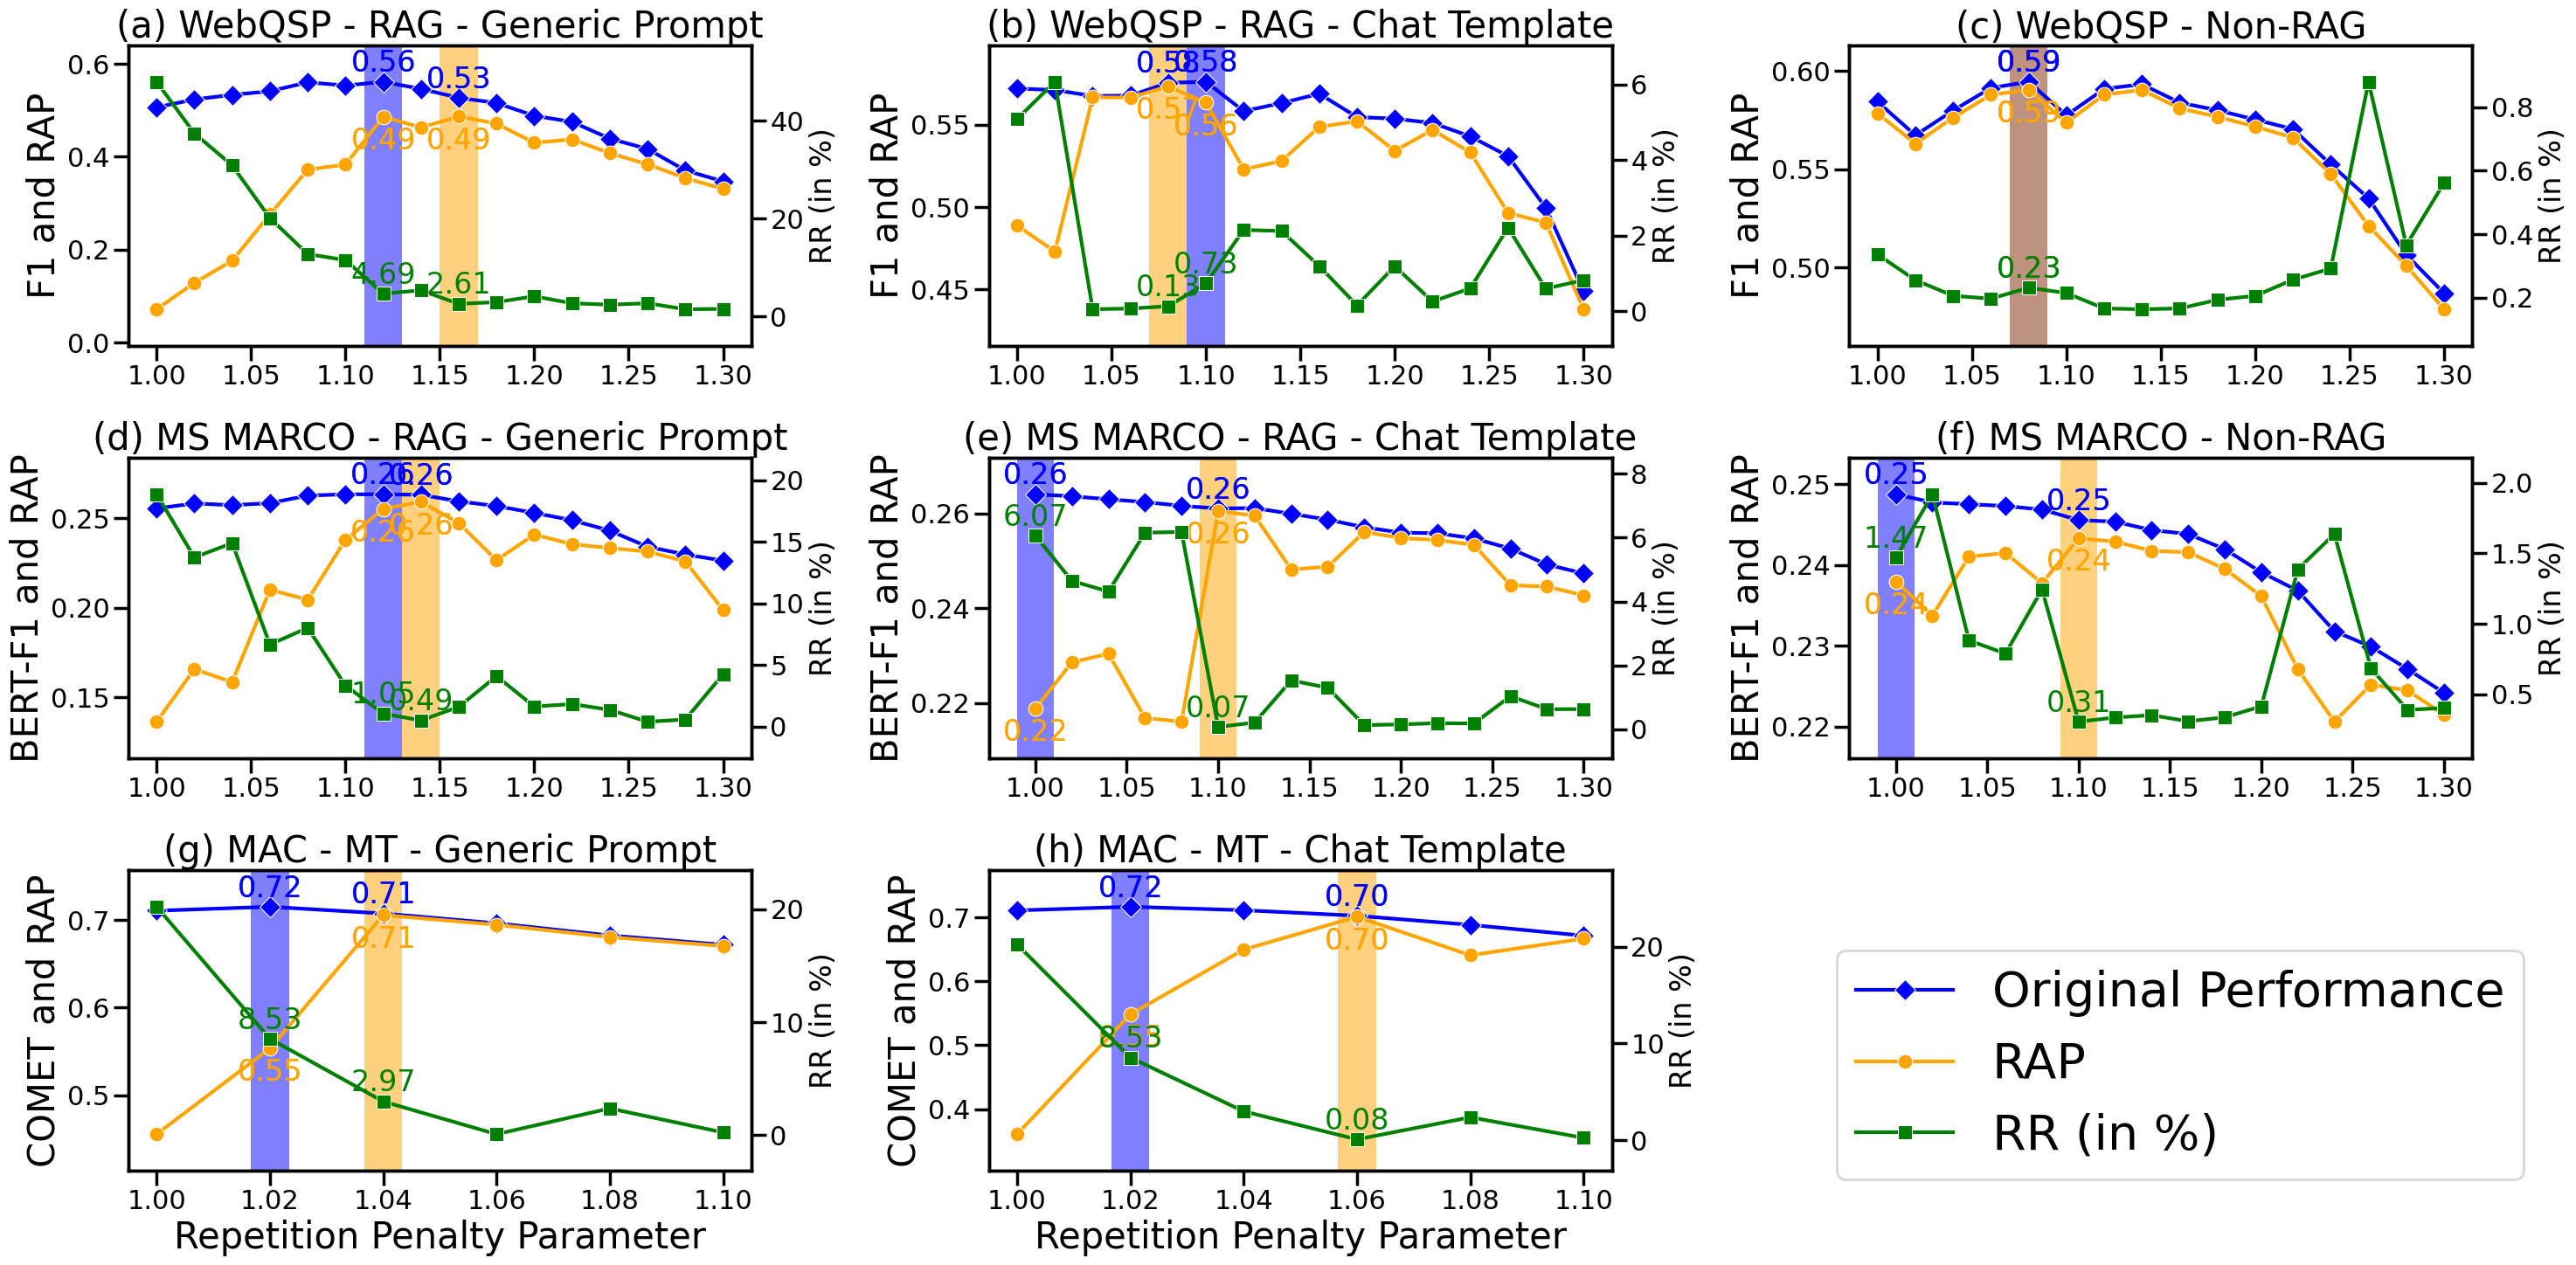
\includegraphics[width=1\textwidth]{image/performance_vs_repetition_v2.png}
    \caption[Performance vs. Repetition Trade-Off]{
    Illustrating original performance, repetition-aware performance (RAP), and repetition ratio (RR) while varying \rpp. Results are shown for Phi-3-mini in QA (Subplots (a) to (f)) and Phi-3.5-mini  in machine translation (Subplots (g) and (h)).
    % Illustrating the original performance, repetition-aware performance (RAP), and repetition ratio (RR) when varying \rpp. Results are shown for the Phi-3-mini model in QA (Subplots (a) to (f)) and the Phi-3.5-mini model in machine translation (Subplots (g) and (h)). 
    % The blue line indicates original performance (F1, BERT-F1, or COMET), the orange line represents RAP, and the green line shows RR in percentage. 
    The blue shaded region highlights the RPP for optimal original performance, while the orange region indicates the RPP for the best RAP; overlapping regions are marked in brown to show alignment.
    % Performance vs. Repetition Trade-Off. This figure shows the original performance and repetition-aware performance (RAP), and the repetition ratio (RR) when varying \rpp, across different datasets and prompt types. We showcase results from Phi-3-mini model for question answering (a-f) and Phi-3.5-mini model for machine translation (g-h) tasks. 
    % The blue line represents the original performance (F1, BERT-F1, or COMET), the orange line represents RAP, and the green line shows \rr in percentage. 
    % The blue shaded region highlights the Repetition Penalty Parameter (RPP) for the best original performance, while the orange region highlights the RPP for the best RAP. When both regions overlap, the shaded area changes to brown to indicate this alignment. 
    % Performance vs. Repetition Trade-Off. This figure shows the balance between performance and repetition reduction across different datasets and prompt types. 
    % Subplots (a-c) present results for the Phi-3-mini model on the WebQSP dataset, and subplots (d-f) show results on the MS MARCO dataset, both with different prompting strategies. Subplots (g-h) illustrate results for the Phi-3.5-mini model on the MAC machine translation task, using various prompting strategies.
    % The blue line represents the original performance (F1, BERT-F1, or COMET), the orange line represents the Repetition-Aware Performance (RAP), and the green line shows the Repetition Ratio (RR) in percentage. 
    % The blue shaded region highlights the Repetition Penalty Parameter (RPP) for the best original performance, while the orange region highlights the RPP for the best RAP. When both regions overlap, the shaded area changes to brown to indicate this alignment. 
    }
    \label{fig:performance_vs_repetition_v2}
\end{figure*}
% We conducted experiments on various datasets and models, comparing performance using both original metrics (such as F1, BLEU, and COMET) and RAP.
% }
% When tuning using conventional metrics, the objective is purely to select the value of \rpp with best performance, but that might come with serious repetition problem. Whereas, 
% Our objective is to identify the optimal \rpp that maximizes RAP by balancing model performance with the reduction of repetition in the generated content.
%
% In this section, we demonstrate the use of \rap in tuning \rpp by comparing model performance and repetition issues when tuning RPP using conventional evaluation metrics versus \rap. 
% Figure \ref{fig:performance_vs_repetition_v2} illustrates the relationship between \rpp, model performance, and repetition across different datasets and prompt strategies. We showcase results of Phi-3-mini for WebQSP and \ms, and Phi-3.5-mini for MAC. 
% The blue lines represent the original performance scores (F1 for WebQSP, BERT-F1 for MS MARCO, and COMET for MAC), the orange lines show the \rap scores, and the green lines (scaled on the right y-axis) indicate \rr in percentage. 
% The blue shaded region highlights the \rpp for the best original performance, while the orange region highlights the RPP for the best RAP. When both regions overlap, the shaded area changes to brown to indicate this alignment. 

This section demonstrates the use of RAP in tuning RPP by comparing model performance and repetition when using conventional metrics (Original Performance) versus RAP. Figure \ref{fig:performance_vs_repetition_v2} shows the relationship between RPP, performance, and repetition for Phi-3-mini on WebQSP and MS MARCO, and Phi-3.5-mini on MAC. Blue lines represent original performance (F1 for WebQSP, BERT-F1 for MS MARCO, and COMET for MAC), orange lines show RAP scores, and green lines (right y-axis) indicate RR percentages. The blue shaded area marks the RPP with the best performance based on conventional metrics, the orange marks the best RAP, and brown indicates overlap between the two.

% In most of the shown cases (except for Figure \ref{fig:performance_vs_repetition_v2}c) the best values of \rpp when tuning using original performance are different from that when tuning using \rap. For example, in Figure \ref{fig:performance_vs_repetition_v2}e, when tuning using BERT-F1, the best \rpp is 1.0 where the performance is \todo{xx}, but the repetition ratio is very high at \todo{xx\%}. Whereas, using \rap, the best \rpp is 1.1, where the performance is \todo{xx} (drop \todo{xx\%}) but the repetition ratio drop significantly to \todo{xx\%} (drop \todo{xx\%)}. This shows that tuning \rpp using \rap helps find \rpp value that minimally reduce performance while significantly lowering repetition ratio. Another example with different visualization is illustrated in Figure \ref{fig:hook}. 

In most cases (except Figure \ref{fig:performance_vs_repetition_v2}c), the optimal RPP differs when tuning for original performance versus RAP. For instance, in Figure \ref{fig:performance_vs_repetition_v2}e, tuning with BERT-F1 gives the best RPP at 1.0 with a performance of 0.264, but the repetition ratio is high at 6.07\%. With RAP, the best RPP shifts to 1.1, where performance drops by 1.1\% (drop 0.003), but the repetition ratio significantly decreases by 98.8\% (drop 6\%). This demonstrates that tuning RPP with RAP helps balance performance with reduced repetition. Another example with different visualization is illustrated in Figure \ref{fig:hook}. 
These results highlight the importance of tuning RPP to balance performance and repetition reduction, which can be achieved using RAP. The optimal RPP varies by task, dataset, and prompting strategy. 

% These results underscore the importance of carefully tuning the RPP to achieve an optimal balance between model performance and repetition reduction, that can be achieved by tuning RPP based on \rap. The optimal RPP value varies depending on the task, dataset, and prompting strategy used.

% \noindent \textbf{WebQSP}: For WebQSP with RAG-Generic Prompt (subplot a), performance remains high up to an RPP of approximately 1.12 before declining, while RR decreases significantly. In contrast, the RAG-Chat Template (subplot b) shows more stable performance across a wider range of RPP values, with lower overall repetition.

% \noindent \textbf{MS MARCO}: The results for MS MARCO (subplots d-f) follow similar trends. RAG-Generic Prompt exhibits a more pronounced trade-off between performance and repetition compared to RAG-Chat Template and Non-RAG approaches.

% \noindent \textbf{MAC}: In the MAC machine translation task (subplots g-h), increasing the RPP beyond certain thresholds (around 1.02–1.04) leads to noticeable declines in performance, while effectively reducing repetition. Both Generic Prompt and Chat Template strategies show similar trends, with higher RPP reducing repetition but negatively impacting COMET scores beyond 1.04.

% Across all datasets and strategies, there is a clear trend of decreasing RR as RPP increases. However, an excessively high RPP can lead to performance degradation. The optimal RPP, typically marked by the peak of the RAP curve (orange line) and highlighted by the orange region in the subplots, often strikes a balance between maintaining high performance and minimizing repetition.

% These results underscore the importance of carefully tuning the RPP to achieve an optimal balance between model performance and repetition reduction, which can be achieved by finding the RPP that maximizes RAP. The optimal RPP value varies depending on the task, dataset, and prompting strategy used.

% \begin{figure*}[ht]
% \centering
% 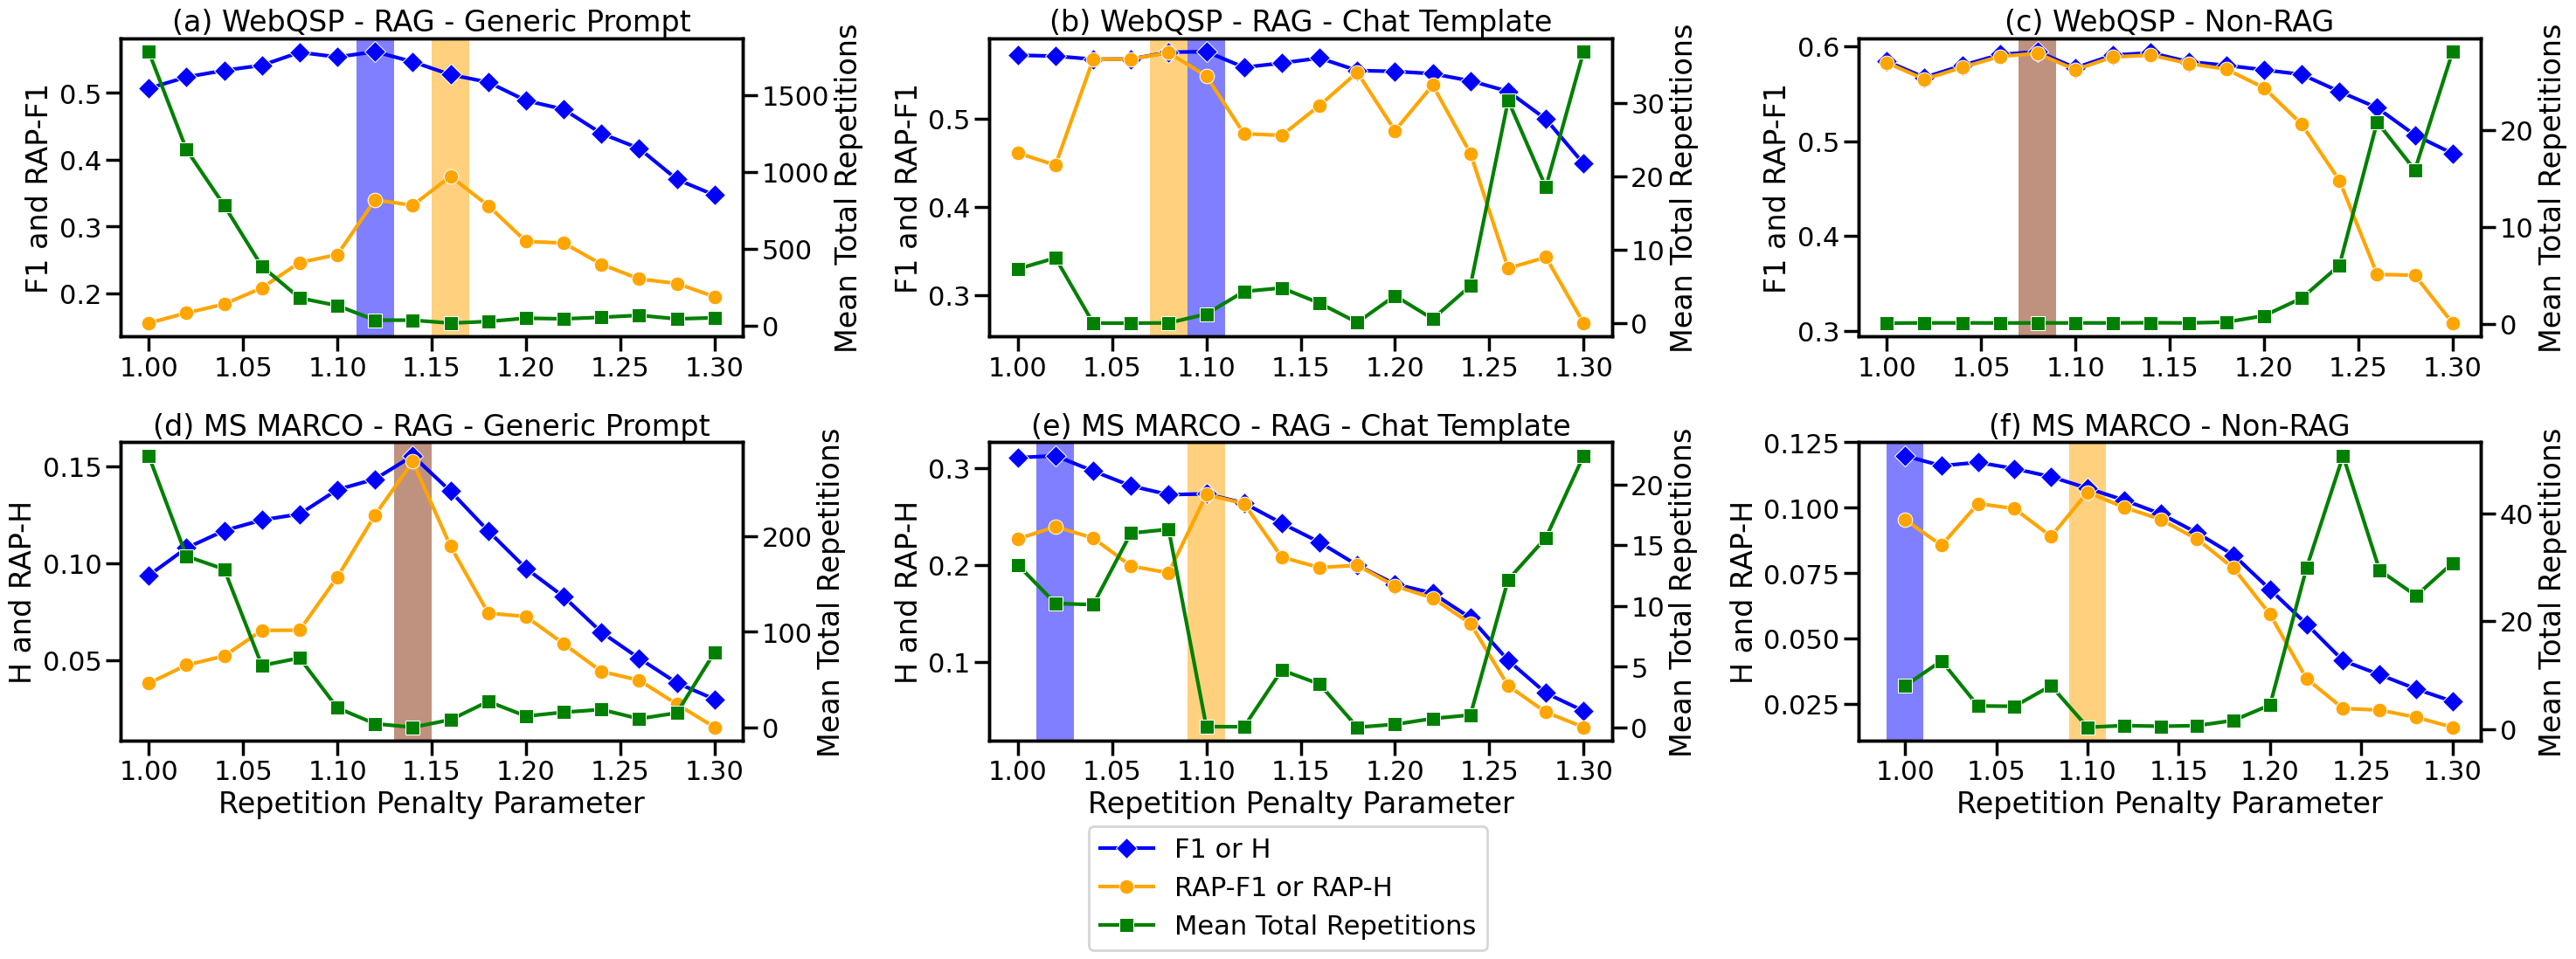
\includegraphics[width=\textwidth]{image/RPP Tuning.png}
% \caption[Performance vs. Repetition Trade-Off]{This figure illustrates the balance between performance and reducing excessive repetition for the Phi-3-mini model across various datasets and prompt types. The blue line is for F1, the orange line is for \mtr, and the green line indicates \rap. These visualizations help discern how a model’s performance and repetition behavior vary with different RPP values.}
%Performance vs. Repetition Trade-Off. This figure illustrates the balance between performance and reducing excessive repetition for the Phi-3-mini model across various datasets and prompt types. The blue lines represent the original performance (F1 or overall performance) scores, the orange lines (scaled on the right y-axis) denote the mean total repetitions (MTR) across the dataset, and the green lines indicate the repetition-aware performance (RAP), which is the original performance adjusted by $\log_{10}(10 + \alpha \times \text{MTR})$, with $\alpha$ fixed at 1 in this study. In these graphs, the blue vertical bar is centered around the RPP (Repetition Penalty Parameter) that yields the best original performance, while the orange bar is positioned at the RPP with the best RAP. In subplots (a), (b), (e), and (f), these two bars are distinctly separated, whereas in subplots (c) and (d), they overlap, resulting in a combined color (likely brown) due to the blending of blue and orange. These visualizations help discern how a model’s performance and repetition behavior vary with different RPP values, thereby aiding in determining the optimal prompts and RPP settings for any AI task.
% \label{fig:performance_vs_repetition}
% \end{figure*}



% \begin{figure*}[ht]
% \centering
% 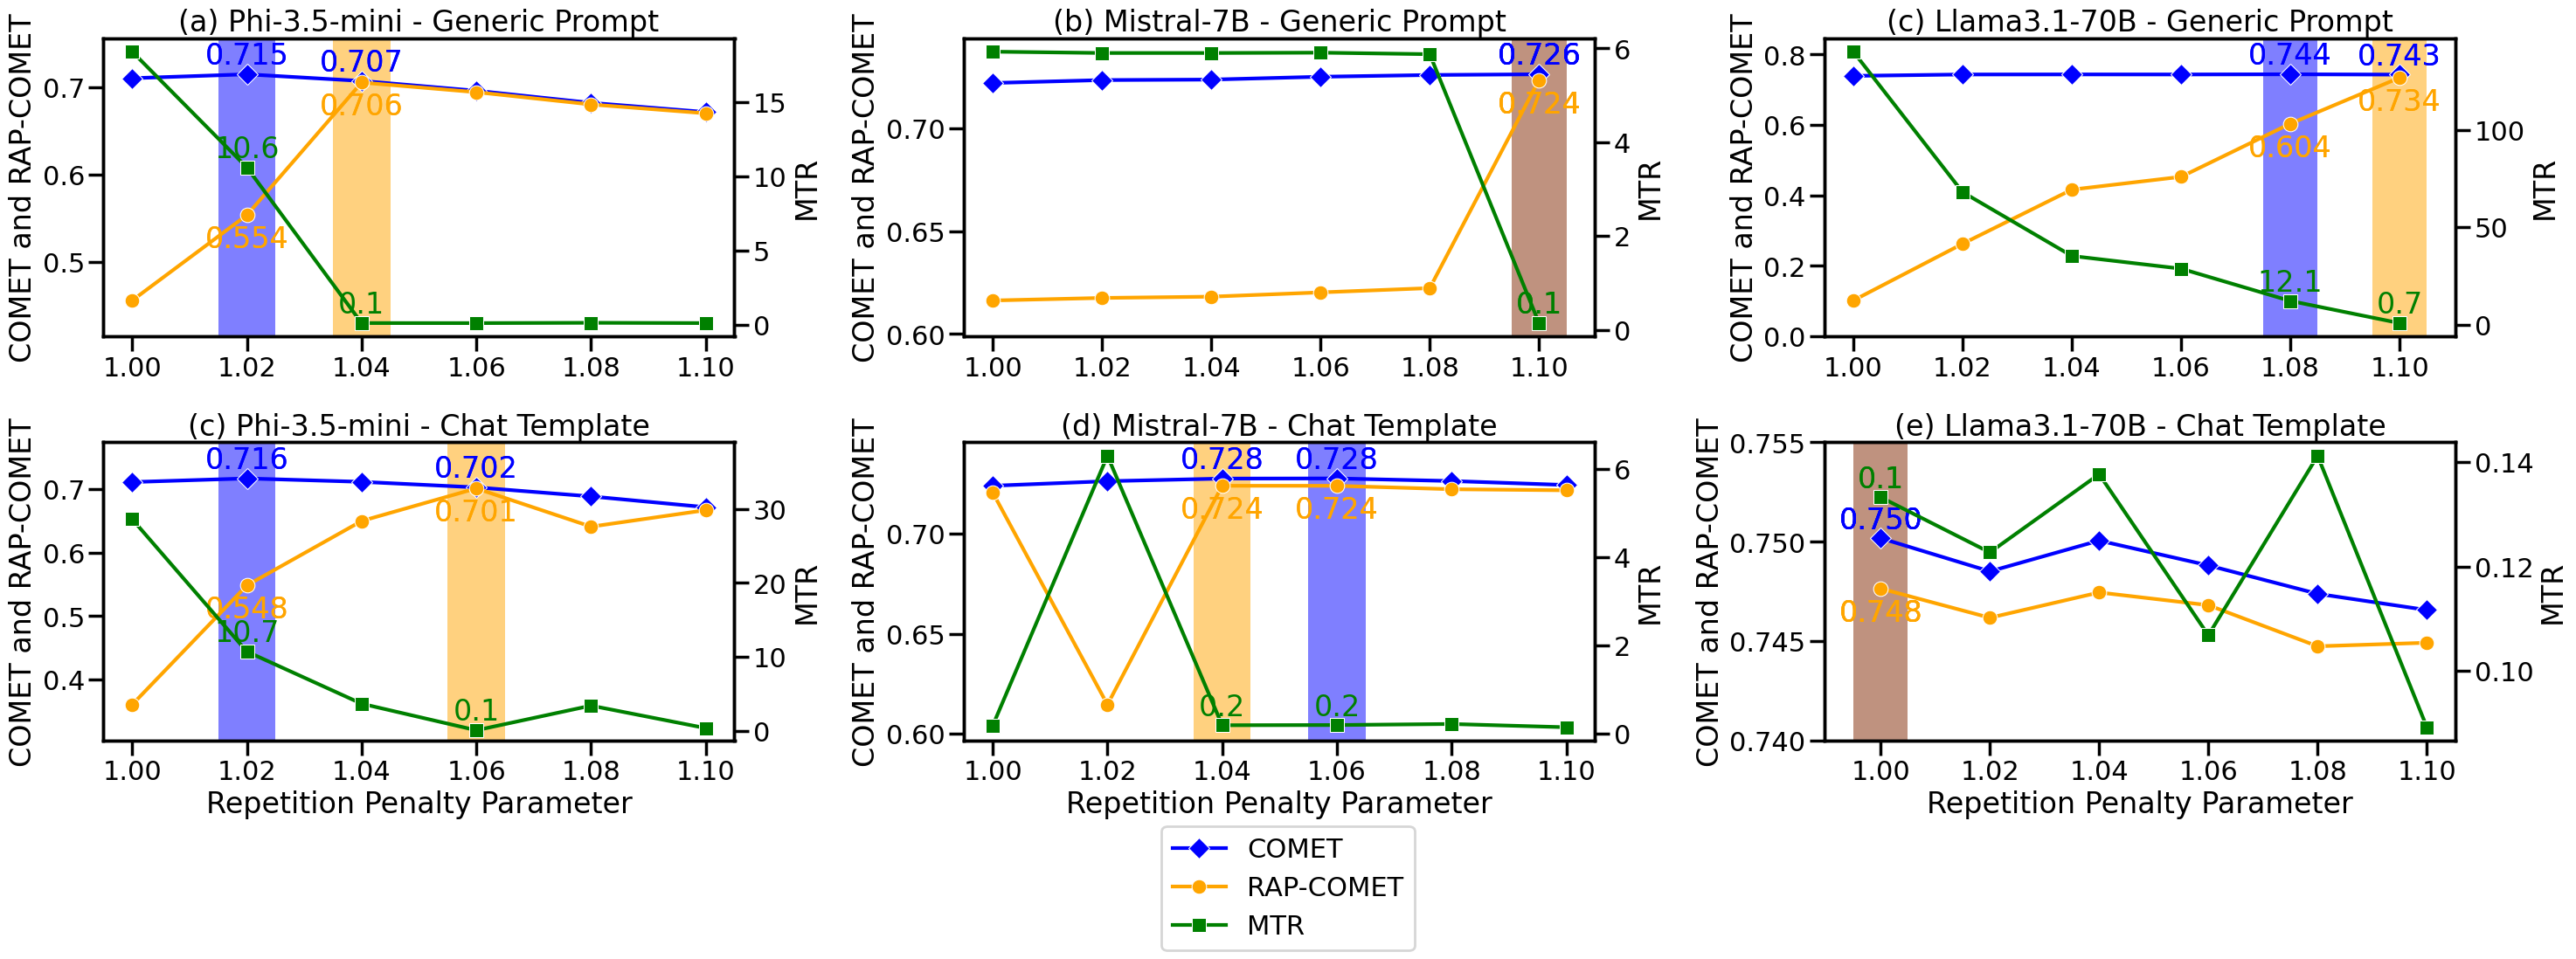
\includegraphics[width=\textwidth]{image/performance_vs_repetition_mt.png}
% \caption[Performance vs. Repetition Trade-Off for MT Tasks]{\new{Performance vs. Repetition Trade-Off for MT Tasks. This figure illustrates the trade-off between performance and the reduction of excessive repetition for the Phi-3.5-mini, Mistral-7B, and Llama3.1-70B models across both Generic Prompt and Chat Template prompt types. The blue line represents COMET, the orange line represents \mtr, and the green line represents \rap. The blue shaded region highlights the Repetition Penalty Parameter (RPP) for the best COMET performance, while the orange region highlights the RPP for the best RAP-COMET performance. When both bars overlap, the shaded region changes to brown to indicate this alignment.}}
% \label{fig:performance_vs_repetition_mt}
% \end{figure*}

% \subsection{Comparing the Best Repetition-Aware Performance of All the Models}
% \todo{@Donghao: to add table of best performance based on RAP. Maybe can use this section to compare the methods, use table. So this is to give people a sense of how the models perform, quantivatively}
% Performance Comparison based on Best \rap
% Comparing Performances of All Models selected based on best \rap. }
% Compare the Performance using tuned RPP (based on RAP)
% \input{tab_best_rpp_v2}
% \input{tab_best_rpp_v3}
% \input{tab_best_rpp_v4}

\subsection{Comparing the RAP-Tuned Performance of All Models}
Table \ref{tab:model-performance} shows the performance of the open-source LLMs after tuning \rpp using \rap. 
On \textbf{WebQSP}, Mistral-7B leads for both \raggen and \ragtem, scoring 0.609 and 0.604, respectively. However, Llama-3-70B outperforms all models in the \nonrag prompt with a high F1 score of 0.710. 
For \textbf{MS MARCO}, Gemma-1.1-2B excels in both \ragtem and \nonrag, with scores of 0.277 and 0.250, while Llama-3-70B takes the top spot in \raggen with 0.275.
In the MT task (\textbf{MAC}), Llama3.1-70B dominates both the generic prompt and chat template categories, scoring 0.743 and 0.750.
These results show that larger models like Llama-3-70B and Mistral-7B consistently achieve top performance across datasets and prompting strategies. However, mid-sized models like Gemma-1.1-2B perform competitively on specific tasks, such as MS MARCO, highlighting that model choice should be task-dependent and not solely based on model size.


% In this section, we analyze the RAP-tuned performance of various models on two different tasks: QA (Question Answering) and MT (Machine Translation). Table \ref{tab:model-performance} provides a comprehensive comparison of model performances across different datasets and prompt types. 
% For the QA task, on the \textbf{WebQSP} dataset, the \textbf{Mistral-7B} model achieves the highest performance for \raggen and \ragtem, with scores of 0.609 and 0.604, respectively. The best \nonrag performance is observed from \textbf{Llama-3-70B}, scoring an impressive 0.710.

% On the \textbf{MS MARCO} dataset, \textbf{Gemma-1.1-2B} achieves top performance for both \ragtem and \nonrag, with scores of 0.277 and 0.250, respectively. The best \raggen score for MS MARCO is achieved by \textbf{Llama-3-70B}, with a score of 0.275.

% For the MT task, \textbf{Llama3.1-70B} dominates, showing the highest performance for both \mtgen and \mttem, with scores of 0.743 and 0.750, respectively.

% These results demonstrate that larger models like \textbf{Llama-3-70B} and \textbf{Mistral-7B} consistently deliver top performance across various datasets and prompt types. However, mid-sized models such as \textbf{Gemma-1.1-2B} also perform competitively, especially on specific tasks like MS MARCO, suggesting that model selection should be guided by task-specific needs and performance trade-offs rather than size alone.




% Our proposed framework, \ours, enables tuning \rp to find the trade-off between repetition and performance, as shown in Section \ref{sec:eval_tuning}. Now, we compare the performances of all the open-source LLMs using the \rp, selected based on \rap. 
% Table \ref{tab:best_rpp} compares the performance of the open-source LLMs across two datasets, WebQSP and MS MARCO, using different prompting strategies: \raggen, \ragtem, and Non-RAG. 
% %
% For the WebQSP dataset, Mistral-7B achieves the best results with both \raggen and \ragtem strategies. In the Non-RAG category, Llama-3-70B excels. Notably, the best result for non-RAG prompting is higher than that in RAG. We argue that since we provide information retrieved from documents instead of a knowledge graph, it might not be sufficient to answer questions from KBQA task that would requires many relational information. This can be seen in the opposite observation in \ms dataset where both RAG prompting strategies obtain much higher scores than non-RAG. 
% The table also highlights the performance penalties due to repetition. For instance, Phi-3-mini using \raggen has an F1 score of 52.7, but its \rap drops to 37.5 due to repetition. A similar trend is observed with Gemma-1.1-7b under the \raggen strategy.
% We also present the best results tuned based on the original F1 scores for \webqsp (denoted as [MODEL-NAME]-F1). This is to demonstrate the potential impact of not considering repetition when tuning \rp. We observed that using our framework, \ours, significantly reduces the repetition issue, with minimal changes in overall performance. For instance, with Llama-2-7B \raggen, an \rp of 1.0 yields the best F1 score of 60.1 but has a high repetition rate of 78.48 on average. However, using \ours, we can select the \rp of 1.06 which drastically reduces the mean total repetition to 0.01, while still achieving a comparable F1 score of 58.9. Several other similar cases are highlighted in blue text, illustrating the effectiveness and benefits of our framework in balancing repetition and performance.
% \todo{to revise, remove framework, to use metric}
% Our proposed framework, \rap, allows tuning \rp to balance repetition and performance, as shown in Section \ref{sec:eval_tuning}. We compare the performances of all open-source LLMs using the selected \rp based on \rap.
% Table \ref{tab:best_rpp} shows the performance of these LLMs across WebQSP and MS MARCO datasets with different prompting strategies: \raggen, \ragtem, and Non-RAG. For WebQSP, Mistral-7B performs best with \raggen and \ragtem, while Llama-3-70B excels in Non-RAG. Interestingly, the best Non-RAG result is higher than RAG, likely because document retrieval may not provide sufficient relational information needed for KBQA tasks. This contrasts with the MS MARCO dataset, where both RAG strategies outperform Non-RAG.
% The table also shows the performance penalties due to repetition. For example, Phi-3-mini using \raggen has an F1 score of 52.7, but its \rap drops to 37.5 due to repetition, a trend also seen with Gemma-1.1-7b under \raggen.
% We also present the best results tuned based on original F1 scores for \webqsp, denoted as [MODEL-NAME]-F1, to show the impact of not considering repetition when tuning \rp. Using our metric, \rap, significantly reduces repetition with minimal performance changes. For instance, with Llama-2-7B \raggen, an \rp of 1.0 yields an F1 score of 60.1 but has a high repetition rate of 78.48. However, with \ours, an \rp of 1.06 reduces repetition to 0.01, still achieving an F1 score of 58.9. Other similar cases are highlighted in blue, demonstrating our framework’s effectiveness in balancing repetition and performance.

% For the MS MARCO dataset, the performance trends shift. The Llama-3-70B model stands out under the \raggen strategy, achieving the highest F1 (33.7) and RAP (33.7) scores. Gemma-2B and Mistral-7B perform best for the RAG-Chat Template and Non-RAG strategies, respectively. There are significant drops from RAG to non-RAG performances. This is due to the difficulty of \ms questions and the high quality of relevant data provided in RAG prompts for \ms. 
% Overall, for both WebQSP and MS MARCO, most models exhibit zero or very low repetition (MTR), demonstrating the effectiveness of \ours in choosing \rp for balancing repetition and performance.



% \subsection{RAG with Chat Template vs Generic Template}
% \subsection{RAG (template or generic, depending on if we can have more results for template WebQSP) with non-RAG}
% \subsection{Repetitions of different settings}
% Can show the differences between different repetition detection methods (method 1 vs method 3 vs method 3.2)
% \subsection{Adjusted results vs original}

% \subsection{Ablation study of what Penalty function should be used?}
% \todo{@Donghao: to add figure + discussion of penalty functions}

% \todo{move to appendix}
% In this section, we qualitatively evaluate the quality of KBQA evaluation generated by Gemini (Section \ref{sec:gemini}). Table \ref{tab:gemini_eval} show examples of output from Llama 3-70B for five \webqsp questions and the corresponding evaluation from Gemini. In the first example, Gemini is able to extract answer-item is ``Lawrence E. Roberts'', and generate the correct mapping between predicted answer and ground-truth answer, this leads to a correct evaluation. Another correct evaluation is obtained in the second example. However, sometimes Gemini fails to extract correct information from generated text. For example, in the third question, Gemini extracted ``Elizabeth Bowes-Lyon'' is also a predicted answer-item, although from the LLM response, we can see that this is not. This leads to giving this answer with 0.5 precision only, hurting the overall performance of the LLM. Another such cases can be seen in the fifth question where Gemini extracted many keywords from the LLM response, this makes the final score is very low, even though by reading the response, we see that the predicted answer was correct. 
% To better understand the quality of our LLM-based KBQA evaluation method, we randomly select 100 samples from the experiment results of Llama-3-70B Non-RAG as this setting obtains the best performance on \webqsp. Then, we ask a human user if the user agree with Gemini's evaluation (similar to the analysis we have done above). The agreement is \textbf{89.0\%}. This shows that although not perfect, our LLM-based KBQA evaluation method has some level of reliability which can be used for KBQA evaluation task.  
% \subsection{Evaluate the Quality of Gemini's Evaluation} 
% \label{sec:eval_gemini}
% To evaluate the quality of our LLM-based KBQA evaluation method, we randomly selected 100 samples from the experiment results of Llama-3-70B Non-RAG, as this setting achieved the best performance on WebQSP. We then asked a human user to review and agree with Gemini’s evaluation (similar to the analysis described above). The agreement rate was 89.0\%, indicating that while not perfect, our LLM-based KBQA evaluation method demonstrates a level of reliability that can be utilized for automatically evaluating LLM responses in the KBQA task. For more details of the actual output from Gemini, please see Section \ref{sec:a_gem} in Appendix. 



% E.g., manually check X samples. Or how? Can mention some question are returned NONE for evaluation. Pick 50 questions, ask human (3 of us?, 3 * 50 or 3*20) to do the same task as Gemini, then we measure precision, recall of Gemini. \todo{to select 150 questions from Llama 3 70B Non RAG, assign 50 to each of us}

% \subsection{Further Discussions}

\subsection{How Severe can Repetition be?}
\begin{figure}[ht]
    \centering
    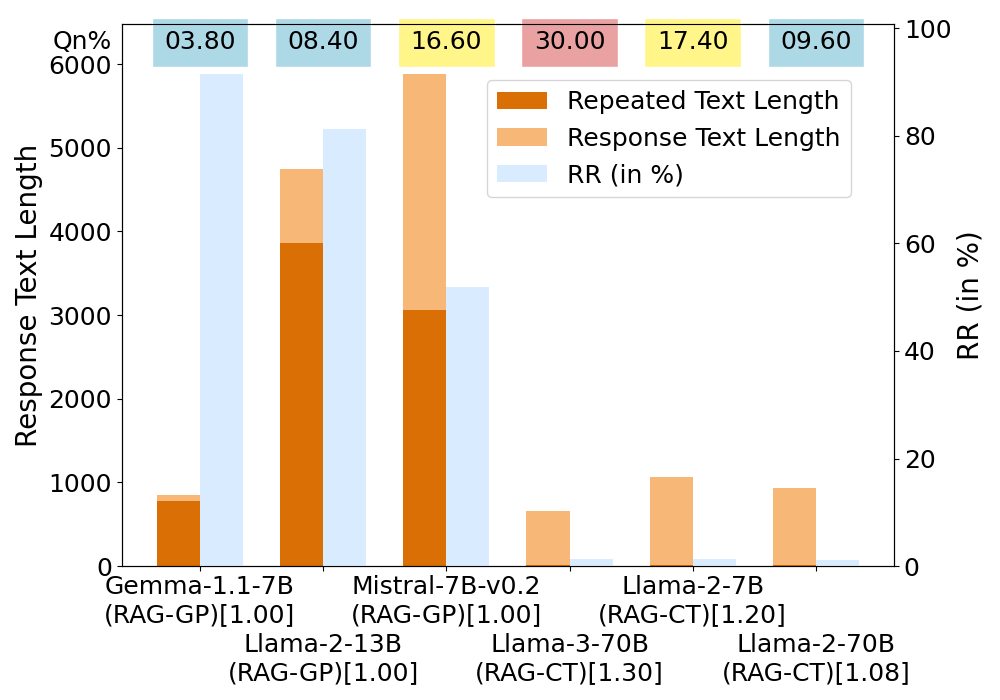
\includegraphics[width=1\linewidth]{image/chart_02_mm.png}
    \caption{
    Severity of repetition. Colored squares above indicate the percentage of repetitive responses. X-label contains model, prompting method, and tuned \rpp.
    % , and the x-label includes the model, prompting method, and tuned value for \rpp. 
    % The severity of repetition. The leftmost three models have the highest RR for \ms, while the rightmost three have the lowest, along with the repetition ratio (y-axis-right) and text length (y-axis-left). Colored squares above each point indicate the percentage of repeated responses, and the x-label includes the model, prompting method, and tuned value for \rpp. 
    % 
    % The severity of repetition. The leftmost three models show the Top-3 highest RR for MS MARCO, while the rightmost three display the lowest. The ratio of repeated text length to text length is also visualized. Colored squares above each point indicate the percentage of repeated questions, with blue, yellow, and red squares marking values below 10\%, between 10-20\%, and above 20\% respectively. The x-label indicates the model, the prompting method, and the RP of the RR. The chart for other models and dataset can be viewed in the appendix.
    }
    \vspace{-1em}
    \label{fig:msmarco_top3}
\end{figure}
In our experiments, the length of text repeated can account for up to 97.85\% of the overall text output, while the proportion of responses with repetition across the entire dataset can reach 41.27\%. Figure \ref{fig:msmarco_top3} shows the top-3 highest and lowest RR for \ms. Colored squares above each point indicate the percentage of repeated responses, with blue, yellow, and red squares marking values below 10\%, between 10-20\%, and above 20\%, respectively. Notably, while Gemma-1-1.7B (RAG-GP) has only 3.8\% of responses with repetition, the repeated text case is very severe as it makes up 91.53\% of the overall answer length. In contrast, 30\% of Llama-3-70B (RAG-CT)'s responses contains repetition, but the repeated text only constitutes 1.29\% of the overall length. The length of repeated content can also be substantial. For instance, Llama-2-13B generated repeated content that averaged around 4,000 characters. 

\subsection{Ablation Study: the Effects of Different Penalty Functions}
\begin{figure}[ht!]
    \centering
    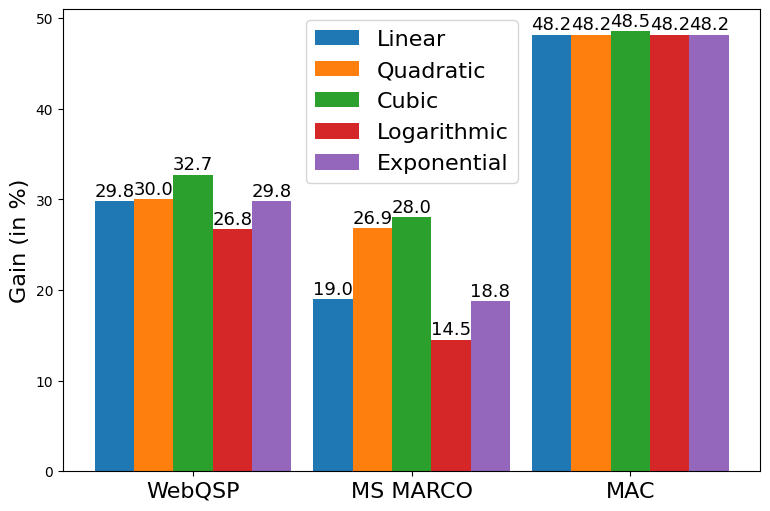
\includegraphics[width=\linewidth]{image/ablation_study.png}
    \caption{Gains across different penalty functions. \textit{Cubic} penalty obtains the best gains across three datasets.}
    \label{fig:ablation_study}
    % \vspace{-1em}
\end{figure}

We now present an ablation study to evaluate the impact of different formulas for the penalty function $F(\rr)$ on \rap (Equation \ref{eq:rap}). We consider five options including \textit{Linear}, \textit{Quadratic}, \textit{Cubic}, \textit{Logarithmic}, and \textit{Exponential} where the penalty are $1-\rr$, $(1-\rr)^2$, $(1-\rr)^3$, $\text{log}_{2}(2-\rr)$, and $e^{-\rr}$, respectively. 
%
We compare the \textit{Gain} achieved with each repetition penalty formula. For a model, \textit{Gain} is defined as the difference between the reduction in repetition and the performance drop when tuning RPP using original performance versus RAP. It reflects how much repetition decreases (i.e., gain) relative to the performance loss when tuning RPP with RAP. The higher \textit{Gain}, the better. 
%
Figure~\ref{fig:ablation_study} shows the \textit{Gain} scores for each formula across the three datasets. The \textit{Gain} for a dataset is calculated by averaging the \textit{Gain} values from all models and prompting strategies. 
% The results show that the \textit{Cubic} penalty consistently achieves the highest gain across all datasets (32.7\% for WebQSP, 28.0\% for MS MARCO, and 48.5\% for MAC), indicating it offers the best balance between reducing repetition and maintaining performance. Notably, all penalty formulas perform similarly well on MAC, with gains around 48\%, suggesting the choice of penalty is less critical for tasks where performance is less sensitive to repetition reduction like MAC. These findings support using the \textit{Cubic} penalty for the RAP metric as it provides a strong balance across varied datasets and tasks.
The results show that the \textit{Cubic} penalty consistently achieves the highest gains across all datasets (32.7\% for WebQSP, 28.0\% for MS MARCO, and 48.5\% for MAC), offering the best balance between reducing repetition and maintaining performance. These findings recommend the \textit{Cubic} penalty for the RAP metric, as it performs well across diverse datasets and tasks.

% The results show that \textit{Cubic} penalty consistently achieves the highest gain across all three datasets (32.7\% for WebQSP, 28.0\% for MS MARCO, and 48.5\% for MAC). This indicates that the cubic function provides the most optimal balance between reducing repetition and preserving model performance.
% Interestingly, all penalty functions perform similarly well on MAC, with gains hovering around 48\%. This suggests that the choice of penalty function may be less critical for tasks or datasets where performance is less sensitive to repetition such as MAC. 
% These findings support our choice of the \textit{cubic} penalty function for the RAP metric, as it provides a robust balance between repetition reduction and performance preservation across diverse datasets and tasks.




% The results highlight several key findings:

% \noindent \textbf{Superiority of Cubic Penalty:} The \textit{cubic} penalty function consistently achieves the highest gain across all three datasets (32.74\% for WebQSP, 28.03\% for MS MARCO, and 48.54\% for MAC). This indicates that the cubic function provides the most optimal balance between reducing repetition and preserving model performance.

% \noindent \textbf{Consistency Across MAC Dataset:} Interestingly, all penalty functions perform similarly well on the MAC dataset, with gains hovering around 48\%. This suggests that the choice of penalty function may be less critical for tasks or datasets where performance is less sensitive to repetition, such as in the MAC dataset.

% \noindent \textbf{Variation Across Datasets:} The \textit{logarithmic} and \textit{exponential} penalty functions exhibit varied performance across datasets. While they perform relatively well on the MAC dataset, they lag behind the polynomial functions (linear, quadratic, and cubic) on both WebQSP and MS MARCO, indicating that the effectiveness of these functions may be task- or dataset-dependent.

% These findings support our choice of the \textit{cubic} penalty function for the RAP metric, as it provides a robust balance between repetition reduction and performance preservation across diverse datasets and tasks.




% The \textit{Gain} is defined as the difference of repetition ratio deduction and performance deduction, i.e., how much repetition drop versus how much performance drops, the large \textit{Gain}, the better. 



% \rap integrates \rr into the overall model performance by applying a penalty function to repetition in the generated content, as defined in Equation~\ref{eq:rap_generic}.

% \begin{equation}
%     \text{RAP} = P \times f(x)
%     \label{eq:rap_generic}
% \end{equation}

% Where $P$ is the performance metric (e.g., F1 score), $f(x)$ is a penalty function, and $x = 1 - \text{RR}$.

% We evaluated the following penalty functions:

% \begin{align}
%     f_{\text{linear, quadratic, cubic}}(x) &= x^n \quad \text{where} \, n \in \{1, 2, 3\} \\
%     f_{\text{logarithmic}}(x) &= \log_2(1 + x) \\
%     f_{\text{exponential}}(x) &= e^{x - 1}
% \end{align}

% We define the \textit{gain} as:

% \begin{equation}
%     \text{Gain} = \frac{\text{RR}_{\text{original}} - \text{RR}_{\text{RAP}}}{\text{RR}_{\text{original}}} - \frac{P_{\text{original}} - P_{\text{RAP}}}{P_{\text{original}}}
% \end{equation}

% Where $\text{RR}_{\text{original}}$ and $P_{\text{original}}$ are the repetition ratio and performance at the best performance-tuned RPP, while $\text{RR}_{\text{RAP}}$ and $P_{\text{RAP}}$ are the corresponding values at the best RAP-tuned RPP.

% Figure~\ref{fig:ablation_study} presents the results of this ablation study, showing the gains achieved across three datasets—WebQSP, MS MARCO, and MAC—for each penalty function. The goal was to maximize the gain, i.e., to achieve the highest reduction in repetition with minimal performance degradation.

% \begin{figure}[ht]
%     \centering
%     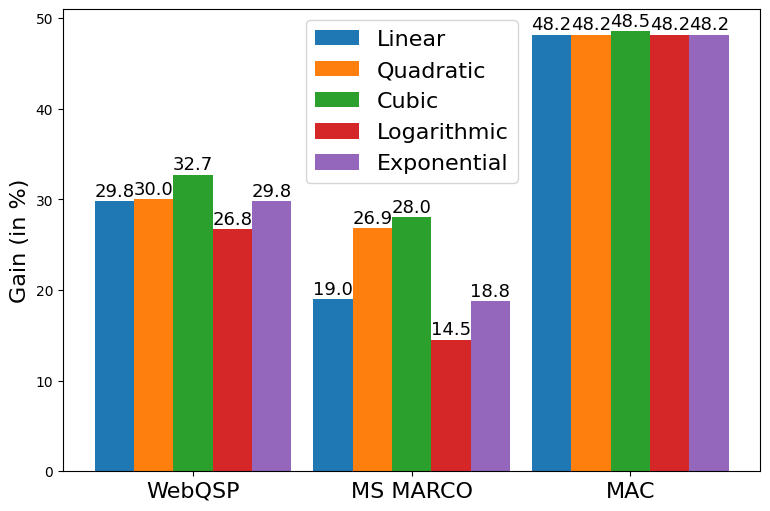
\includegraphics[width=\linewidth]{image/ablation_study.png}
%     \caption{Gains across different penalty functions on three datasets (WebQSP, MS MARCO, and MAC). The evaluated penalty functions include \textit{linear}, \textit{quadratic}, \textit{cubic}, \textit{logarithmic}, and \textit{exponential}.}
%     \label{fig:ablation_study}
% \end{figure}

% The results highlight several key findings:

% \noindent \textbf{Superiority of Cubic Penalty:} The \textit{cubic} penalty function consistently achieves the highest gain across all three datasets (32.74\% for WebQSP, 28.03\% for MS MARCO, and 48.54\% for MAC). This indicates that the cubic function provides the most optimal balance between reducing repetition and preserving model performance.

% \noindent \textbf{Consistency Across MAC Dataset:} Interestingly, all penalty functions perform similarly well on the MAC dataset, with gains hovering around 48\%. This suggests that the choice of penalty function may be less critical for tasks or datasets where performance is less sensitive to repetition, such as in the MAC dataset.

% \noindent \textbf{Variation Across Datasets:} The \textit{logarithmic} and \textit{exponential} penalty functions exhibit varied performance across datasets. While they perform relatively well on the MAC dataset, they lag behind the polynomial functions (linear, quadratic, and cubic) on both WebQSP and MS MARCO, indicating that the effectiveness of these functions may be task- or dataset-dependent.

% These findings support our choice of the \textit{cubic} penalty function for the RAP metric, as it provides a robust balance between repetition reduction and performance preservation across diverse datasets and tasks.
\section{Conclusion}
This research tackles the challenge of reducing repeated content generation while preserving overall performance in open-source LLMs. We propose the repetition-aware performance metric, \rap, which quantifies and integrates repetition penalty into model evaluation. Conventional metrics often overlook repetition, making it difficult to tune the repetition penalty parameter (\rpp). In contrast, RAP enables effective tuning of \rpp and can be easily applied to other repetition methods as well.
%

We evaluated \rap on twelve open-source LLMs using three datasets across QA and MT tasks, with different prompting strategies. Results show that higher RPP values generally reduce repetition but can significantly impact performance. This phenomenon emphasizes the need of tuning \rpp. 
The experiments also demonstrate the capability of using \rap for identifying the \rpp value that efficiently reduce repetition while minimizing performance loss.
We also highlight the severity of the repetition issues in the generated content, calling for greater attention from the research community on this matter.
Our experiments offer valuable insights into managing repetition in open-source LLMs, including a recommendation to use Chat Templates for RAG prompting. We will release the source code and all experimental data, offering a large dataset of LLM-generated content for future research on repetition issues and LLM capabilities in QA and MT tasks.


% This research tackles the challenge of mitigating generating repeated content while minimizing the performance loss for open-source LLMs. we introduce repetition-aware performance, \rap, a metric to quantify and integrate repetition penalty into model performance. Tuning \rpp is not feasible when using conventional evaluation metrics since they do not take into account the repetition issue in these metrics. \rap enables tuning repetition penalty parameter (\rpp). 
% We evaluated the proposed metric for twelve open-source LLM, using three datasets of question answering and machine translation tasks, with different prompting techniques. 
% The experimental results on  show that higher \rpp values generally reduce repetition but may also impact performance significantly. This highlight the need of tuning \rpp to find the trade-off between reducing repetition and losing model performance. The results also so the capability of using \rap for finding \rpp value that efficiently reduce repetition while minimizing performance loss. 
% Our extensive set of experiments provide valuable insights on dealing with repetition in open-source LLMs. We will publish the source code, as well as all the data generated in the experiments. This is a substantial amount of LLM-generated data, that can be used of a resource for other research such as further investigation in repetition issues and the capability of LLMs in question answering and machine translation tasks. 


% By publishing the datasets, RAPGeT source code, and LLM outputs, we aim to support the research community in improving LLM output fidelity and utility. Future work will focus on enhancing ReDA algorithms to detect a wider range of text anomalies and extending RAPGeT to support tasks beyond question answering, such as reasoning and AI agents, thereby broadening its applicability and impact in various AI domains.

% This research has addressed significant challenges in mitigating repetition in large language models (LLMs) by developing the RAPGeT framework, which integrates the repetition factor (RF) with traditional performance metrics. Our experiments show that higher Repetition Penalty Parameter (RPP) values generally reduce repetition but may also impact performance, highlighting the need for a balanced approach. The framework's fast and reliable repetition detection algorithm provides immediate feedback, facilitating dynamic adjustment of repetition penalties. Our practical evaluation toolset, rigorously tested across diverse LLMs and multiple QA datasets, offers valuable insights for optimizing LLM performance without compromising content quality. By publishing the datasets, RAPGeT source code, and LLM outputs, we aim to support the research community in improving LLM output fidelity and utility. Future work will focus on enhancing ReDA algorithms to detect a wider range of text anomalies and extending RAPGeT to support tasks beyond question answering, such as reasoning and AI agents, thereby broadening its applicability and impact in various AI domains.
\newpage

\section{Limitations}
This study has several limitations. First, while we conducted experiments with twelve open-source LLMs, our findings may not be generalizable to other open-source models or newer architectures due to variations in design and training data. This limitation suggests that further research could explore a wider array of models to validate the applicability of our findings.

Second, our current repetition detection method focuses solely on non-word character and text repetition. This may overlook other relevant forms of repetition, such as word salad repetition, which could further impact the quality of generated content. Addressing these additional types of repetition in future work could lead to a more comprehensive understanding of repetition issues in LLMs.

Third, this research examines two specific tasks: question answering and machine translation. While these tasks are significant, extending the study to include other applications, such as text summarization, could provide deeper insights into LLM behavior concerning text repetition across various NLP tasks. This expansion would help in understanding how different tasks may influence repetition patterns and the overall performance of LLMs.

Finally, this work concentrates on the repetition penalty parameter (\rpp). However, other methods, such as sampling techniques, temperature adjustments, and context size modifications, can also be used to mitigate repetition issues in generative models. While \rap can be easily applied alongside these methods, further research evaluating \rap across different repetition control methods would enhance our understanding of how to manage repetition issues in LLMs more effectively.

% Our research has a few limitations worth noting. First, although we have conducted experiments in twelve open-source LLMs, it might still hard to have a generlizable conclusion for other open-source LLMs or newer models. Second, regarding repetition detection, currently we only consider non-word character and text repetition, however, it could have more type of repetition, such as, word salad repetition. Third, in this paper, we study two tasks of question answering and machine translation. Extending this study to other applications like text summarization could provide more understanding LLMs' behaviors in generating text repetition across different NLP tasks.

    % First, 
    % we focused on a limited selection of open-source LLMs, which might make it harder to generalize our findings to proprietary or newer models; expanding this scope in future studies could provide more insights. Second, while the repetition ratio (RR) is a cool new metric, we haven’t fully explored how it stacks up against more established ones, so future work should look into how RR correlates with and maybe even enhances other metrics in different linguistic contexts. Lastly, adding our repetition detection algorithm could introduce some computational overhead, which might affect the performance and scalability of LLMs. Future versions of the framework will need to find a good balance between complexity and efficiency for wider use.
    % \item \textbf{Scope of LLMs Tested}: Our study was limited to a selection of open-source LLMs, potentially constraining the generalizability of our findings to proprietary or newly developed language models. Future research could expand this scope to assess the framework’s effectiveness across a broader range of LLMs.
    % \item \textbf{Metric Dependence}: While the repetition ratio (RR) is an innovative addition to performance metrics for LLMs, its effectiveness and reliability relative to more established metrics remain underexplored. Future studies should examine how RR correlates with and possibly enhances other metrics across various linguistic contexts.
    % \item \textbf{Complexity and Performance}: The integration of our repetition detection algorithm may introduce computational overhead, potentially impacting the performance and scalability of LLMs. Future iterations of the framework will need to balance complexity with efficiency to ensure broader applicability.
    % \item \textbf{Adjustment of Repetition Penalties}: Achieving an optimal balance of the repetition penalty parameter (RPP) without manual intervention remains a challenge. This process may benefit from more sophisticated, AI-driven automation techniques in future developments.
    % \item \textbf{Task Specificity}: Our research focused primarily on question-answering tasks. Extending the framework to other applications like summarization could provide a more comprehensive understanding of its utility across different NLP tasks.
    % \item \textbf{False Positives in Repetition Detection}: The current repetition detection algorithm may produce minor false positives when identifying closely related words, such as in the phrase “resolve solve.” Adjusting the threshold for text repetition detection could mitigate this issue. We plan to address this refinement in our future work to enhance accuracy.

% \section*{Acknowledgments}  % to add in the camera-ready (so that not violate double blind review
% \newpage
\bibliography{ref}
\newpage
\appendix
\clearpage
\section{Appendix}
\label{sec:appendix}
% \begin{itemize}
%     \item show RAG templates for all models 
% \end{itemize}

\label{sub:data-col-pre}
% \todo{@donghao: double check appendix}
\subsection{Data Collection and Preprocessing}
\label{sec:data}
% \todo{remove rapget}
We evaluate our proposed metric, \rap, using two tasks of question answering and machine translation. For question answering, we use \webqsp and \ms. The \textbf{\webqsp} dataset \cite{yih2016value} is a widely used benchmark for KBQA task. We selected a subset of 1008 questions from test data, mainly following the criteria as for WebQSP-WD \cite{C18-1280} that to keep questions with at least one acceptable answer in Wikidata. 
% , a subset of WebQSP containing only questions with at least one acceptable answer in Wikidata. We retrieved up to 10 documents per query from Wikipedia for the RAG-based question answering task.
\textbf{\ms} (Microsoft Machine Reading Comprehension) is a comprehensive dataset for reading comprehension and question answering, released by Microsoft\footnote{\url{https://microsoft.github.io/msmarco/}}. For our experiments, we used the dataset created by \cite{huang2024performance}. This dataset includes 100 queries, each with well-formed answers across five categories: LOCATION, NUMERIC, PERSON, DESCRIPTION, and ENTITY, totaling 500 queries. Each query is accompanied by 10 passages that provide context for the RAG-based question answering task.
For machine translation task, we use the \textbf{\mac} (Manually Aligned Chinese-English) dataset curated by \cite{huang2025optimizing}. This dataset comprises sentences from six Chinese novels and their corresponding English translations, spanning a diverse range of genres, including humor, martial arts, classics, war, romance, and science fiction. It contains a total of 5,661 entries, with 4,528 used for training and 1,133 reserved for testing.

\noindent
\textbf{Preparing Context-Data for \webqsp} 
\label{sub:webqsp}
To evaluate open-source LLMs using various prompting strategies, including Retrieval-Augmented Generation (RAG), we crawled Wikipedia for relevant documents to address \webqsp questions. We developed a Python script to prepare the context data by retrieving up to 10 documents per query, which were then processed through text extraction, segmentation, and embedding. These document chunk embeddings were stored locally for vector search. For each question, we retrieved the 8 most relevant document chunks through similarity search to form the context for RAG prompting.

% \begin{enumerate}
% \textbf{WebQSP}: Introduced by \cite{yih2016value}, the WebQuestionsSP (WebQSP) dataset is a widely used benchmark for knowledge-based question answering (KBQA) over structured data. For our experiments, we selected 1008 queries from the WebQSP-WD dataset \cite{C18-1280}, a subset of WebQSP containing only questions with at least one acceptable answer in Wikidata. We retrieved up to 10 documents per query from Wikipedia for the RAG-based question answering task.
% \textbf{MS MARCO}: MS MARCO (Microsoft Machine Reading Comprehension) is a comprehensive dataset for reading comprehension and question answering, released by Microsoft\footnote{\url{https://github.com/microsoft/MSMARCO-Question-Answering\#qa}}. For our experiments, we selected 100 queries with well-formed answers across five categories: LOCATION, NUMERIC, PERSON, DESCRIPTION, and ENTITY, resulting in a test dataset of 500 queries. Each query in the dataset is accompanied by 10 passages used as context for the RAG-based question answering task.
% \end{enumerate}
% The resulting datasets, WebQSP-RAPGeT and MS MARCO-RAPGeT, have very similar structures, each containing the following elements:
% \begin{enumerate}
%     \item \textbf{id}: retrieved from the source dataset
%     \item \textbf{question}: retrieved from the source dataset
%     \item \textbf{answers}: retrieved from the source dataset
%     \item \textbf{context}: for MS MARCO, the context is created by merging the passages from the source dataset. The method for creating contexts for WebQSP is detailed in Section \ref{sub:webqsp}.
% \end{enumerate}
% Regarding ground-truth answers, \ms includes an element called \textbf{wellFormedAnswers} retrieved from the source dataset, which serves as ground truth for performance evaluation using BLEU and Rouge-L scores. Whereas, \webqsp ground-truth answers contain lists of entities

% Additionally, MS MARCO-RAPGeT includes an element called \textbf{wellFormedAnswers} retrieved from the source dataset, which serves as ground truth for performance evaluation using BLEU and RougeL scores.
% 
% Unlike MS MARCO-RAPGeT, the WebQSP-RAPGeT dataset contains only gold entities in the answers element, which are used as ground truths. We developed a novel evaluation method, detailed in Section \ref{sec:gemini}, to assess the generated texts against these entity ground truths.

\noindent


% \subsection{Creation of Context for \webqsp}
% Since we want to evaluate open-source LLMs for different prompting strategies including RAG which requires providing relevant data to the question, we crawl documents from Wikipedia containing relevant information for answering questions in \webqsp. To create the context data element for the \webqsp dataset, we developed a Python script using LangChain\footnote{\url{https://github.com/langchain-ai/langchain}}, a framework designed to simplify the creation of applications using LLMs. The script first retrieved up to 10 documents per query from Wikipedia. These documents were then processed through text extraction, segmentation, and embedding procedures utilizing the LangChain framework and the HuggingFace Instructor text embedding model\footnote{\url{https://huggingface.co/hkunlp/instructor-large}}, resulting in the generation of embeddings. These embeddings, along with the source document chunks, were efficiently stored locally using FAISS\footnote{\url{https://ai.meta.com/tools/faiss}}, an open-source library for vector search created by Meta, which facilitates streamlined document retrieval. The script ran for more than 7 hours to complete processing all 1008 questions. Finally, for each question in the dataset, we used another script to retrieve the 8 most relevant document chunks through similarity search and combined them to form the context while performing RAG prompting.

% We aim to evaluate open-source LLMs for various prompting strategies, including RAG, which requires providing relevant data to the question. To conduct the experiments, we crawled documents from Wikipedia containing pertinent information for answering questions in the \webqsp. We developed a Python script using LangChain\footnote{\url{https://github.com/langchain-ai/langchain}}, a framework designed to simplify the creation of applications using LLMs, to prepare context data for \webqsp questions. 
% The script first retrieved up to 10 documents per query from Wikipedia. These documents were then processed through text extraction, segmentation, and embedding procedures using the LangChain framework and the HuggingFace Instructor text embedding model\footnote{\url{https://huggingface.co/hkunlp/instructor-large}}, resulting in the generation of embeddings. These embeddings, along with the source document chunks, were efficiently stored locally using FAISS\footnote{\url{https://ai.meta.com/tools/faiss}}, an open-source library for vector search created by Meta, which facilitates streamlined document retrieval. The script ran for over 7 hours to complete processing all 1008 questions. Finally, for each question in the dataset, we used another script to retrieve the 8 most relevant document chunks through similarity search and combined them to form the context while performing RAG prompting.

%Processing all 1008 questions took over 7 hours.

\subsection{LLM-based KBQA Evaluation} 
\label{sec:gemini}
% Why it is not straightforward to evaluate LLM's output for this. Because KBQA answers are list of entities, but output is freetext. Propose to use an independent LLM (Gemini) to assist in evaluating. 

\begin{listing}[t]
\begin{minted}[breaklines=true,fontsize=\small]{text}
You are evaluating a question answering task. The ground-truth answer is a list of answer-items. 
First, extract the answer-items from the generated answer. 
Then, map each generated answer-item to the ground-truth answer-item if possible. If no matching, use an empty list.
Output using the following format. {"predicted_answer": [list of answer-items extracted from the generated answer], "mappings": {"predicted_answer_1": [matched groundtruth answers], "predicted_answer_2": []}}

Question: <KBQA Question>
Ground-truth answer: <KBQA Ground-truth Answer>
Generated answer: <LLM-generated Answer>
\end{minted}
\caption{Prompt template for KBQA evaluation using Gemini Pro. The actual content will be filled in the placeholders of \textit{Question}, \textit{Ground-truth answer}, and \textit{Generated answer}. }
\label{list:gemini_prompt}
\end{listing}

\begin{figure}
    \centering
    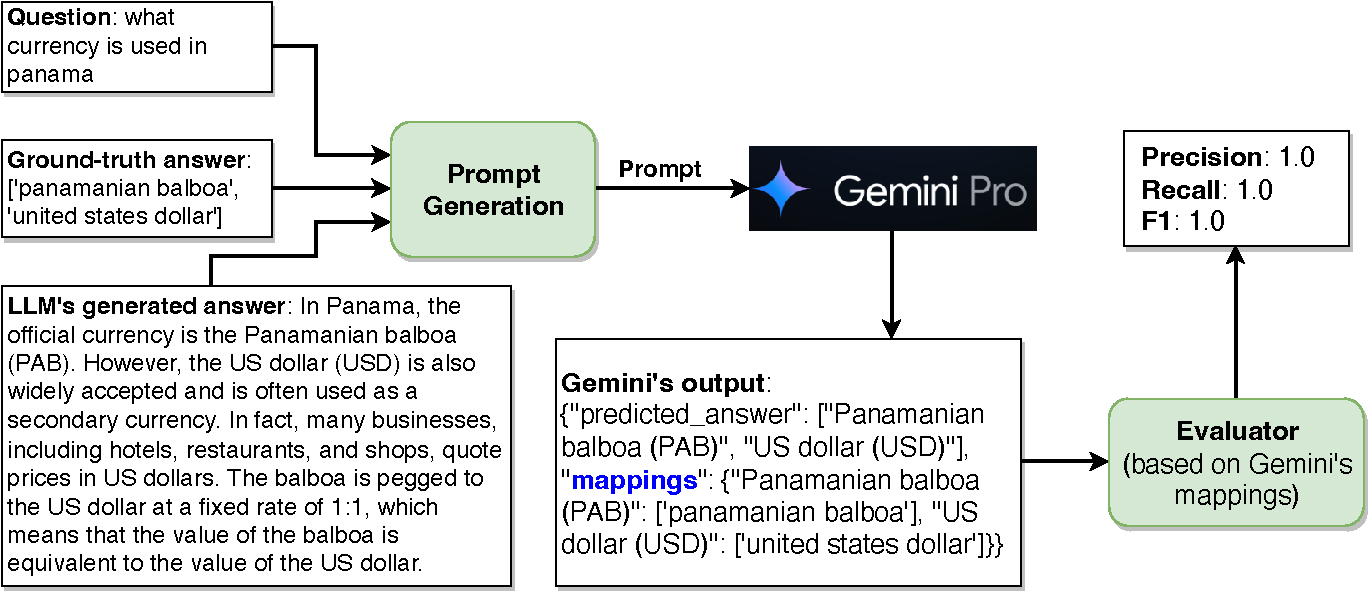
\includegraphics[width=.5\textwidth]{image/gemini_eval.pdf}
    \caption{LLM-based KBQA evaluation workflow using prompts for precision, recall, and F1 scores with Gemini-1.0-Pro as evaluator.}
    %\caption{LLM-based KBQA Evaluation Workflow. Given the input of \textit{question}, \textit{ground-truth answer}, and \textit{LLM's generated answer}, we create a prompt to extract answer-items and map them to ground-truth answer-items. Then, we calculate the precision, recall, and F1 based on the mappings of generated and ground-truth answer-items. We use Gemini-1.0-Pro for this evaluation task.} %The generated answer is taken from Llama 3-8B. }
    \label{fig:gemini_eval}
\end{figure}

% In KBQA task, the most common type of answer is a list of entities from the KG. For example, the answer to the question ``What language is spoken in Switzerland?'' is ``[Italian language, German language, French, Romansh language]''. While we can request LLMs to generate answers in the format of a list of entities, not all LLMs consistently follow this output format request. Therefore, it is crucial to process the answers returned by LLMs to extract the entity list for evaluation. One solution is to use Named Entity Recognition (NER); however, answers can contain other types of information besides named entities. Additionally, the wording used in answers might differ from the KG's entities even though they refer to the same entity, such as ``United States Dollar'' versus ``US dollar (USD)''.

% To resolve this problem, we propose an LLM-based evaluation method where an LLM is requested to extract answer-items (entities) from the generated answer and map them to the ground-truth answer-items. Figure \ref{fig:gemini_eval} shows the LLM-based KBQA evaluation workflow with an actual example using an answer generated from Llama 3-8B. We first construct a prompt using our pre-defined prompt template, shown in Listing \ref{list:gemini_prompt}. The prompt contains the input question, ground-truth answer, LLM's generated answer, and a request to extract answer-items and map them to the ground-truth answer-items. As shown in Figure \ref{fig:gemini_eval}, Gemini outputs a list of \textit{predicted answers} and a \textit{mapping} which maps each item in the predicted answers with those in ground-truth answers. Noted that one predicted answer-item can be mapped to more than one ground-truth answer-item or none (i.e., wrong answer). 

In the KBQA task, answers are typically lists of entities from the KG. For instance, the answer to ``What language is spoken in Switzerland?'' is ``[Italian, German, French, Romansh]''. While LLMs can be asked to generate entity lists, they do not always follow this format. Therefore, processing LLM-generated answers to extract entity lists for evaluation is crucial. Using Named Entity Recognition (NER) alone is not sufficient because answers may include non-entity information and differing entity wordings, e.g., ``United States Dollar'' versus ``US dollar (USD)''.
To address this, we propose an LLM-based evaluation method where an LLM extracts and maps answer-items (entities) from the generated answer to the ground-truth entities. Figure \ref{fig:gemini_eval} illustrates this workflow with an example generated by Llama-3-8B. We construct a prompt using a predefined template (Listing \ref{list:gemini_prompt}), including the question, ground-truth answer, LLM-generated answer, and a request for entity extraction and mapping. As shown in the figure, Gemini outputs a list of \textit{predicted answers} and a \textit{mapping} of predicted answers to ground-truth answers. A predicted answer can map to multiple ground-truth items or none (i.e., incorrect answer).

The mapping is then used to compute evaluation metrics including Precision, Recall, and F1. The details are as follows. 
Given a question, we denote the ground-truth answer as $A=[A_1, A_2, \cdots, A_n]$ and the list of predicted answer-items as $\hat{A}=[\hat{A}_1, \hat{A}_2,\cdots, \hat{A}_m]$. The mapping is denoted as $M=\{\hat{A}_1: M_1, \hat{A}_2: M_2, \cdots, \hat{A}_m: M_m\}$ where $M_i$ is a list of ground-truth answer-items matched with the corresponding predicted answer-item, i.e., $M_i \subseteq A$ ($i=1, \cdots, m$) and $M_i$ is empty when the predicted answer-item is wrong. A predicted answer-item is called \textit{correct} if it matches with at least one of the ground-truth answer-items.
We define $c_G=|\text{set}(M_1\cup M2 \cup \cdots \cup M_m)|$ as the number unique ground-truth answer-items that matched with at least one predicted answer-item and $c_P$ as the number of correct predicted answer-items. The final number of correct answers is chosen as the smallest number between $c_G$ and $c_P$. 
% :
% \begin{align}
%     c = \left\{\begin{matrix}
% c_G & \text{if } c_G < c_P\\ 
% c_P & \text{otherwise} 
% \end{matrix}\right.
% \end{align}
This is to deal with the cases where different predicted answer-items carry the same meaning (mapped to the same ground-truth answer-item). The precision and recall are then computed as $\frac{c}{|\hat{A}|}$ and $\frac{c}{|A|}$, respectively. 
% follows: 
% \begin{align}
%     \text{precision} = \frac{c}{|\hat{A}|}
% \end{align}
% \begin{align}
%     \text{recall} = \frac{c}{|A|}
% \end{align}
F1 score is computed as the harmonic mean of precision and recall. 
We chose \gemini for this evaluation task because of its strong natural language processing capabilities and its availability during our experiments.

\subsection{Tuning RPP for All Models and Datasets}
\label{sec:gain_all}
\begin{figure}[ht]
    \centering
    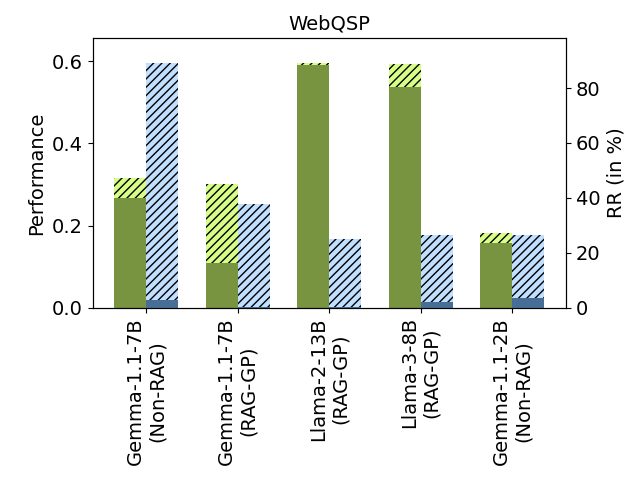
\includegraphics[width=1\linewidth]{image/chart_00_selected_wd.png}
    \caption{Top-5 model with highest RR reduction for \webqsp dataset}
    \label{fig:chart_00_selected_wd}
\end{figure}
\begin{figure}[ht]
    \centering
    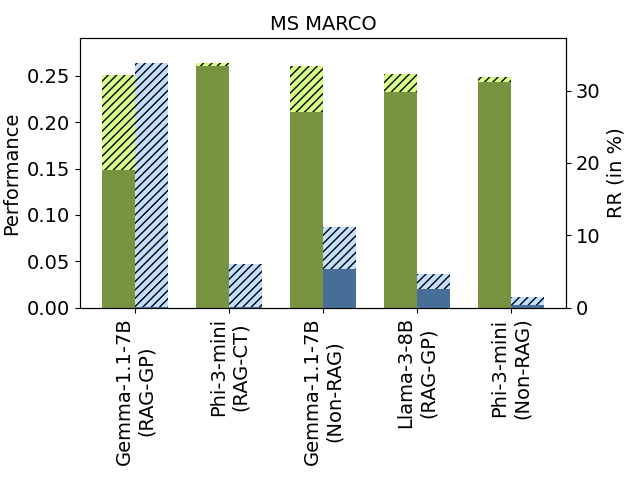
\includegraphics[width=1\linewidth]{image/chart_00_selected_mm.png}
    \caption{Top-5 model with highest RR reduction for \ms dataset}
    \label{fig:chart_00_selected_mm}
\end{figure}
\begin{figure}[ht]
    \centering
    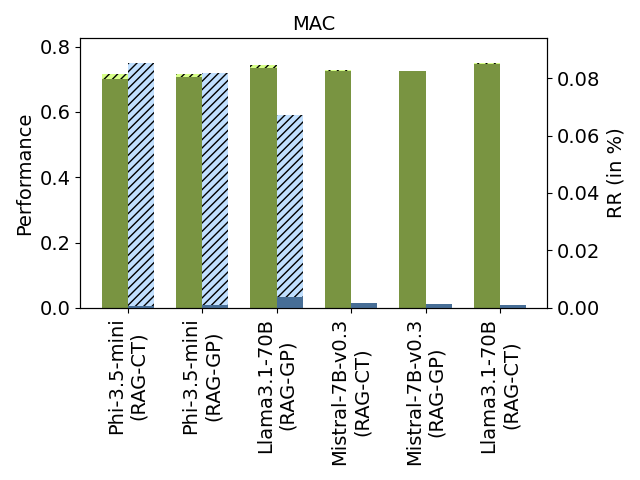
\includegraphics[width=1\linewidth]{image/chart_00_selected_mac.png}
    \caption{Tuning RPP of all models for \mac dataset}
    \label{fig:chart_00_selected_mac}
\end{figure}

We visualize the best performance when tuning RPP using original evaluation metrics (Original) and our proposed repetition-aware performance metric (RAP). RAP helps find RPP values that minimally reduce performance while significantly lowering repetition ratio (RR). Results for all models across three datasets are shown in Figure \ref{fig:chart_00_specific} (\webqsp, \ms) and \ref{fig:chart_00_selected_mac} (\mac). Figure \ref{fig:chart_00_selected_wd} and \ref{fig:chart_00_selected_mm} show the top-5 highest RR reduction after tuning for \webqsp and \ms dataset respectively. Green color bar indicates performance and blue color bar indicates RR. The hatched bar visualize the magnitude of reduction after tuning. 

\subsection{How Severe can Repetition be for Other Models and Datasets?}
\label{sec:how_severe}
Figure \ref{fig:webqsp_top3} visualize the top-3 highest and lowest RR for WebQSP, while Figure \ref{fig:chart_02_wd_all}, \ref{fig:chart_02_mm_all}, and \ref{fig:chart_02_mac_all} visualize all models for \webqsp, \ms, \mac respectively. The leftmost three models show the Top-3 highest RR, while the rightmost three display the lowest. The ratio of repeated text length to text length is also visualized. Colored squares above each point indicate the percentage of repeated questions, with blue, yellow, and red squares marking values below 10\%, between 10-20\%, and above 20\% respectively. The x-label indicates the model, the prompting method, and the RP of the RR. 
\begin{figure}[t]
    \centering
    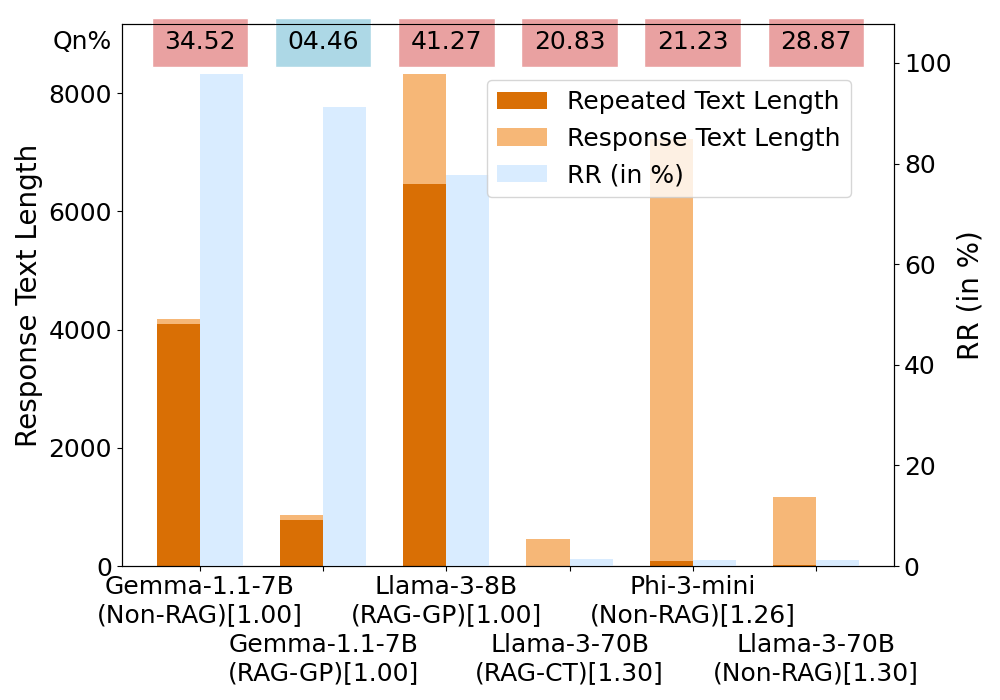
\includegraphics[width=1\linewidth]{image/chart_02_wd.png}
    \caption{Top-3 highest and lowest RR for \webqsp dataset}
    \label{fig:webqsp_top3}
\end{figure}
\begin{figure}[t]
    \centering
    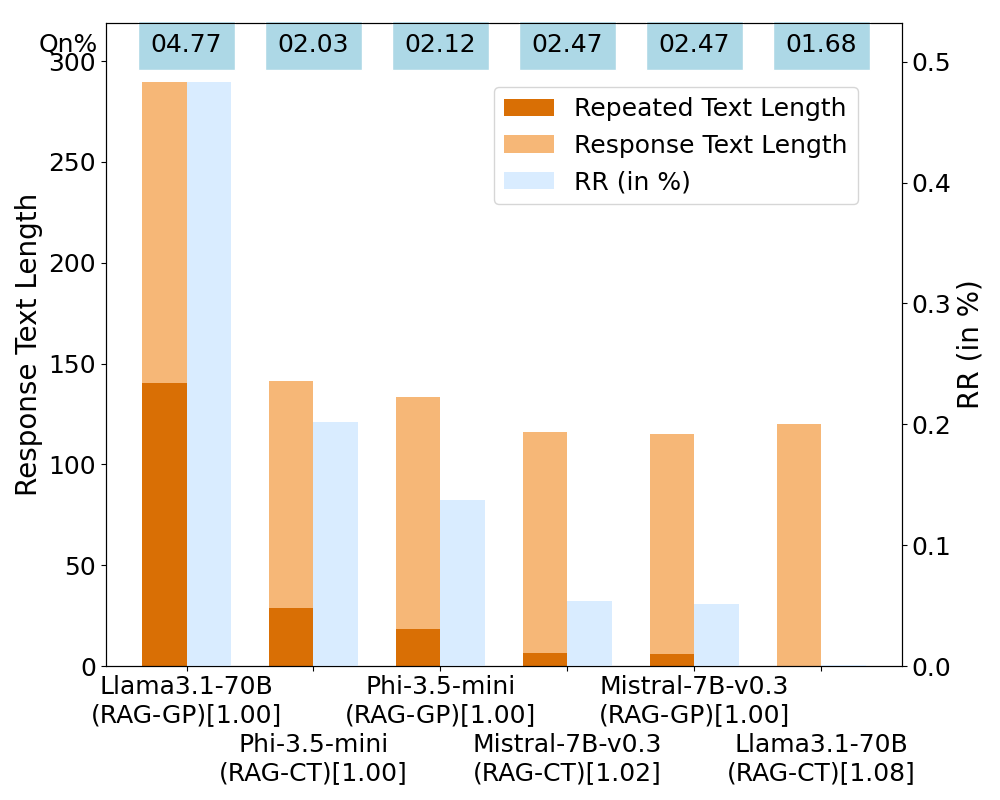
\includegraphics[width=1\linewidth]{image/chart_02_mac_all.png}
    \caption{Percentage of repeated responses, repeated text length, and RR for \mac dataset}
    \label{fig:chart_02_mac_all}
\end{figure}
\begin{figure*}[t]
    \centering
    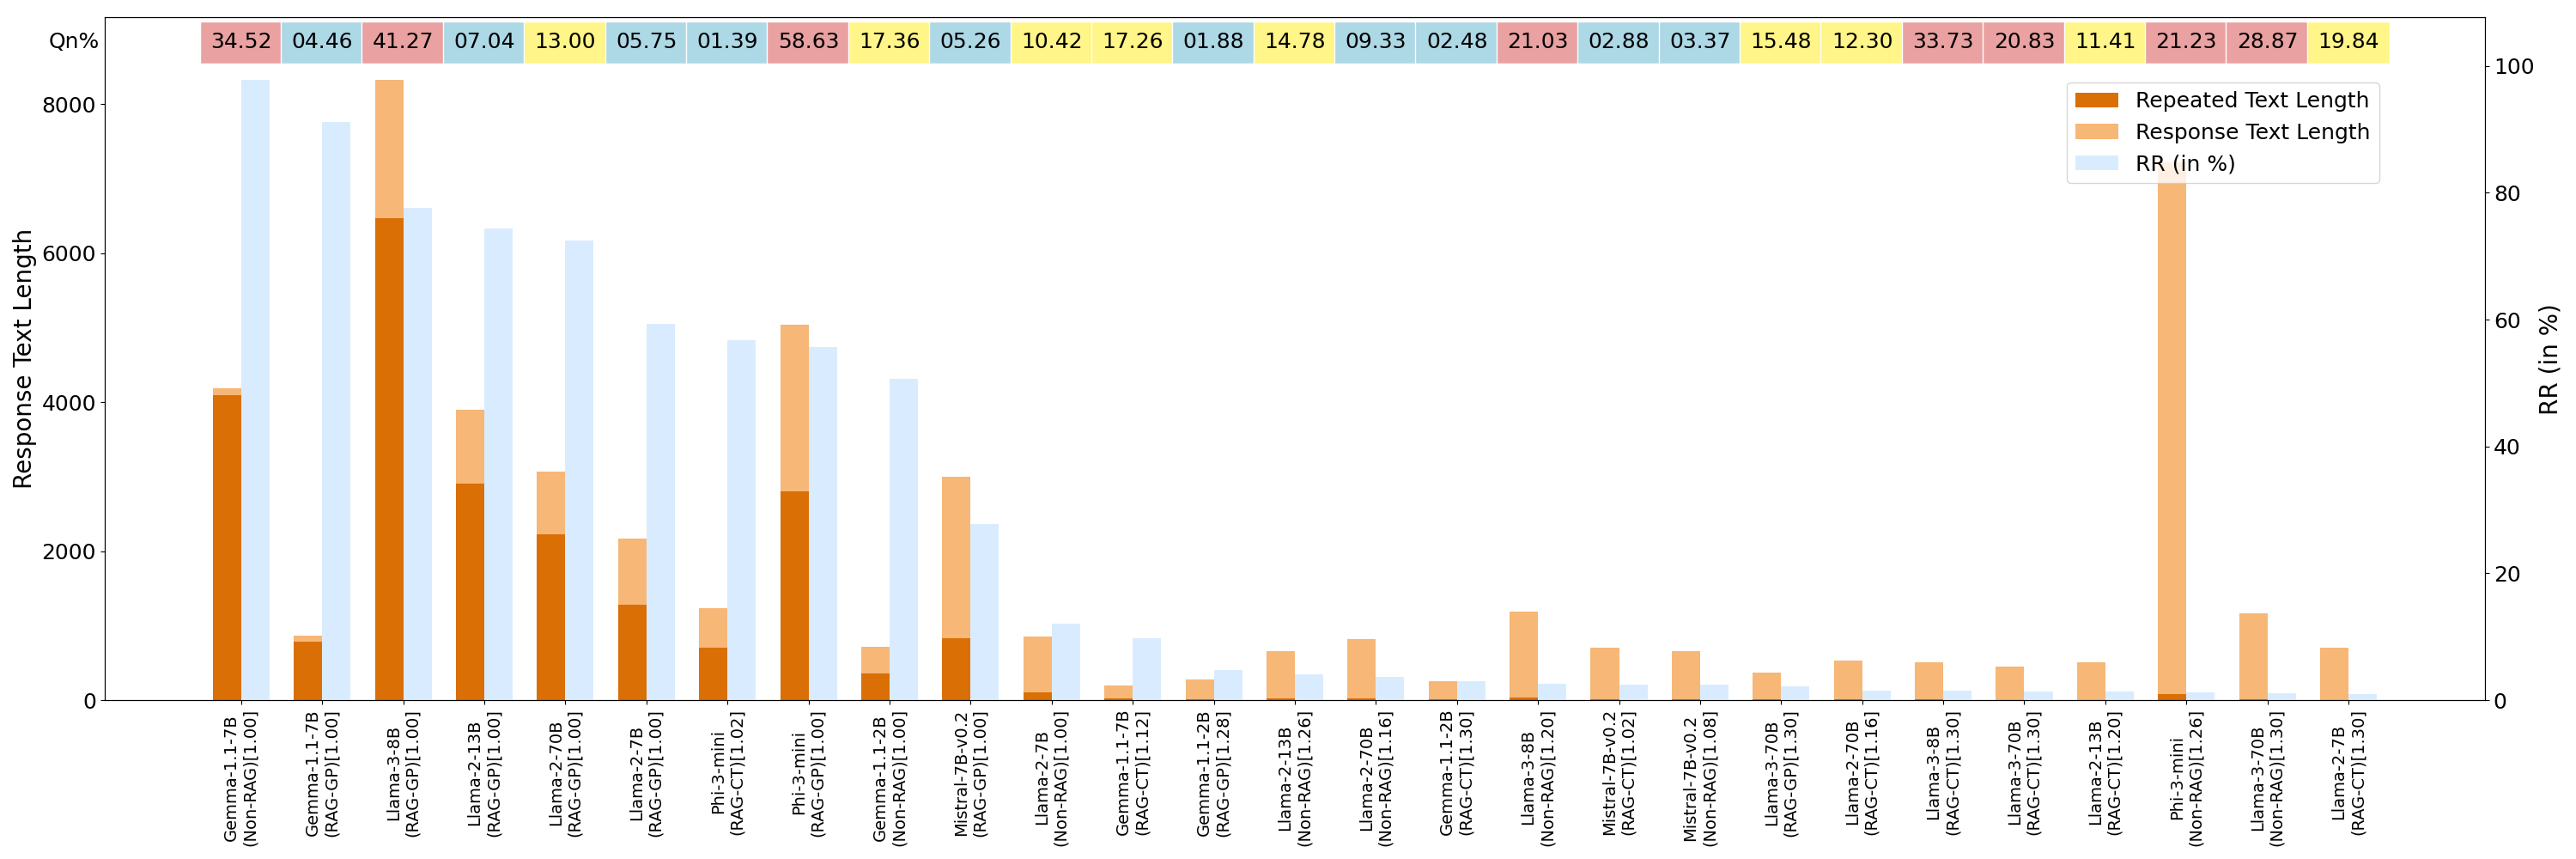
\includegraphics[width=\textwidth]{image/chart_02_wd_all.png}
    \caption{Percentage of repeated responses, repeated text length, and RR for \webqsp dataset}
    \label{fig:chart_02_wd_all}
\end{figure*}
\begin{figure*}[t]
    \centering
    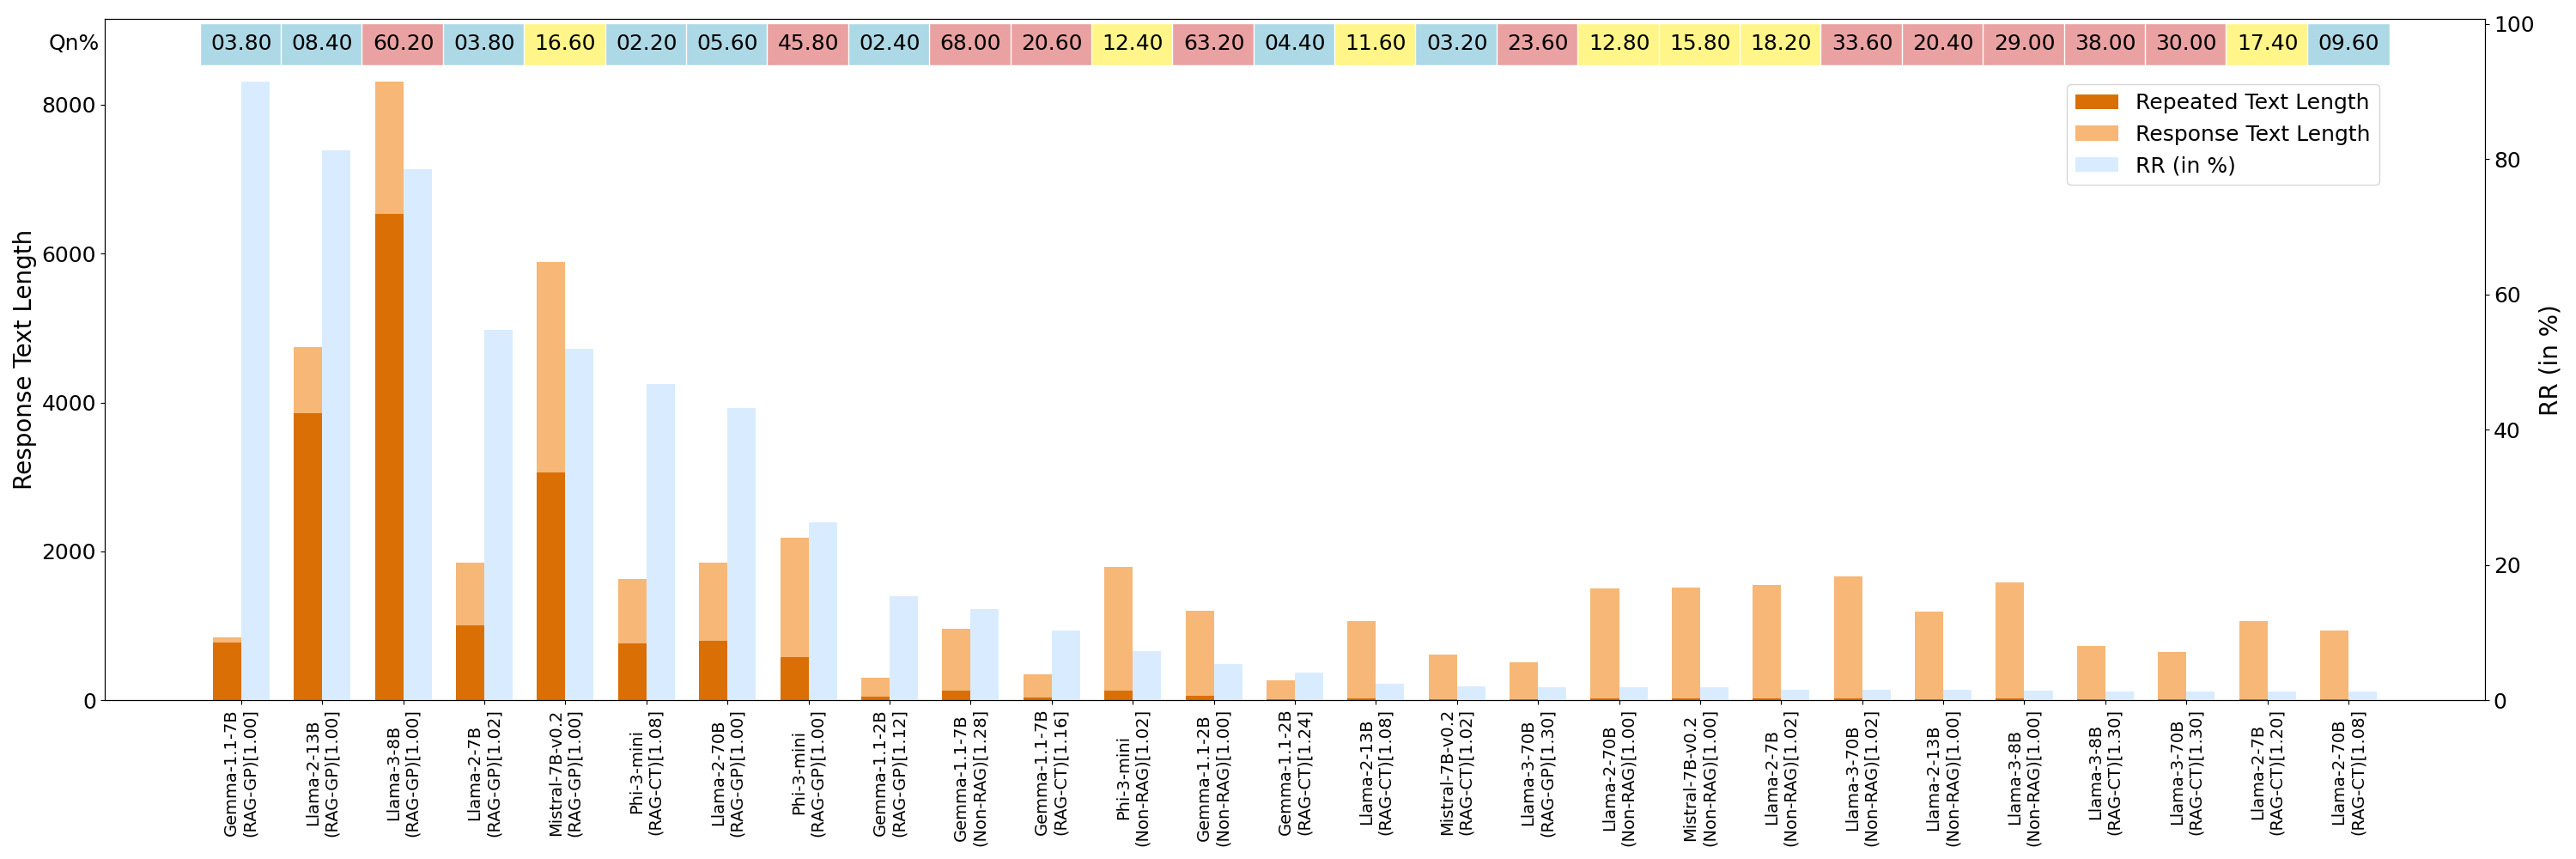
\includegraphics[width=\textwidth]{image/chart_02_mm_all.png}
    \caption{Percentage of repeated responses, repeated text length, and RR for \ms dataset}
    \label{fig:chart_02_mm_all}
\end{figure*}
\begin{figure*}[t]
    \centering
    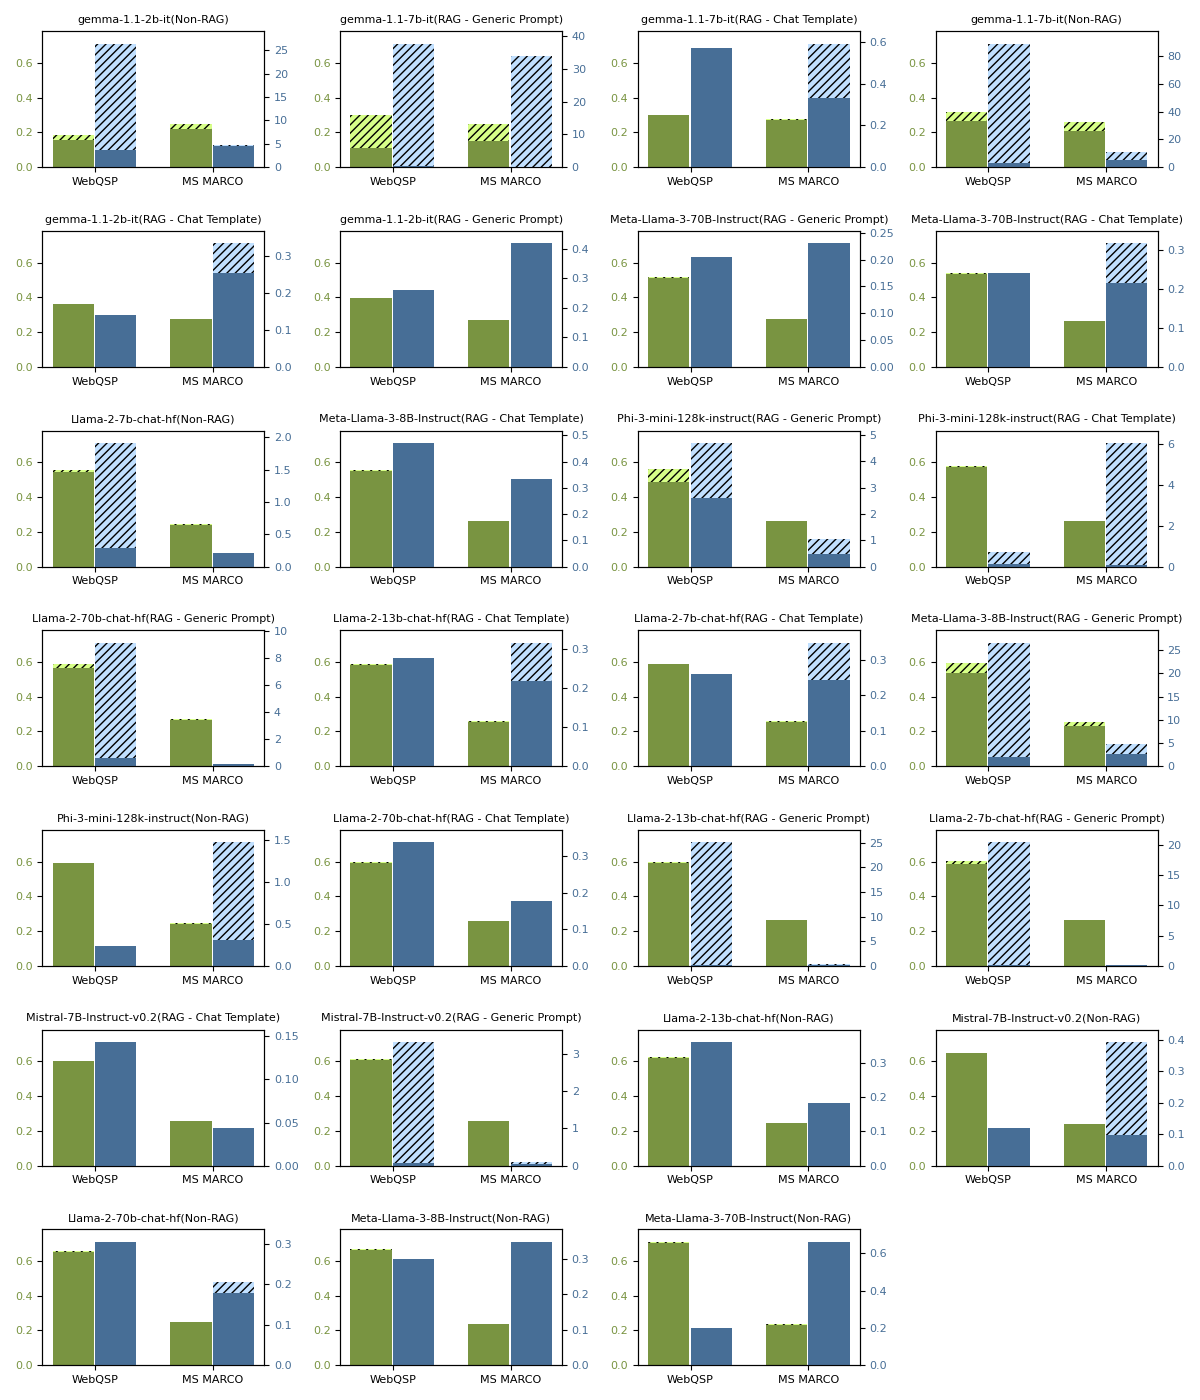
\includegraphics[width=\textwidth]{image/chart_00_specific.png}
    \caption{Tuning RPP of all models for \webqsp and \ms dataset}
    \label{fig:chart_00_specific}
\end{figure*}



\subsection{Evaluating the Quality of Gemini's Evaluation} 
\label{sec:eval_gemini}

To assess the effectiveness of our LLM-based KBQA evaluation method, we randomly selected 100 samples from the experiment results of the Llama-3-70B Non-RAG model, as this configuration achieved the best performance on WebQSP. A human evaluator was then asked to review and provide feedback on Gemini’s evaluation of these samples (following the process described earlier). The agreement rate between the human evaluator and Gemini was 89.0\%. While this indicates that the method is not flawless, it demonstrates a high level of reliability, making our LLM-based KBQA evaluation suitable for automatically assessing LLM responses in KBQA tasks.

\begin{table*}[]
\centering
\small
\resizebox{\textwidth}{!}{
\begin{tabular}{c|p{.1\textwidth}|p{.1\textwidth}|p{.4\textwidth}|p{.4\textwidth}}
\toprule
No. & Question                                     & Ground-truth               & LLM Response (Llama 3-70B)                                                                                                                                                                                                         & Gemini's Evaluation                                                                                                                                                                                                                                            \\ \midrule
1   & who is robin roberts father            & {[}lawrence e. roberts{]}                  & Robin Roberts father is Lawrence   E. Roberts, a pilot in the United States Air Force and a colonel. He passed   away in 2004.                                                                                       & \{\textbf{predicted\_answer}: {[}Lawrence E.   Roberts{]}, \textbf{mappings}: \{Lawrence E. Roberts: {[}lawrence e. roberts{]}\}\}                                                                                                                                           \\\midrule
2   & who does michael oher play for in 2010 & {[}baltimore ravens{]}                     & In 2010, Michael Oher played for   the Baltimore Ravens.                                                                                                                                                             & \{\textbf{predicted\_answer}: {[}Baltimore   Ravens{]}, \textbf{mappings}: \{Baltimore Ravens: {[}baltimore ravens{]}\}\}                                                                                                                                                    \\\midrule
3   & who was queen   elizabeth ii mom       & {[}'queen elizabeth the queen   mother'{]} & Queen Elizabeth II's mother was   Queen Elizabeth The Queen Mother, also known as Elizabeth Bowes-Lyon. She was   the wife of King George VI and the mother of Queen Elizabeth II and Princess   Margaret.           & \{"\textbf{predicted\_answer}":   {[}"Queen Elizabeth The Queen Mother", "Elizabeth   Bowes-Lyon"{]}, "\textbf{mappings}": \{"Queen Elizabeth The Queen   Mother": {[}'queen elizabeth the queen mother'{]}, "Elizabeth   Bowes-Lyon": {[}{]}\}\}                            \\\midrule
4   & where was rihanna born and raised      & {[}saint michael parish{]}                 & Rihanna was born in Saint   Michael, Barbados, and raised in Bridgetown, Barbados.                                                                                                                                   & \{\textbf{predicted\_answer}: {[}Saint   Michael, Bridgetown{]}, \textbf{mappings}: \{Saint Michael: {[}saint michael parish{]},   Bridgetown: {[}{]}\}\}                                                                                                                    \\\midrule
5   & what country was king tut s tomb found & {[}egypt{]}                                & King Tuts tomb, also known as   KV62, was discovered in Egypt. Specifically, it was found in the Valley of   the Kings, a necropolis in Luxor, Egypt, on November 4, 1922, by British   archaeologist Howard Carter. & \{\textbf{predicted\_answer}: {[}Egypt,   Valley of the Kings, Luxor, Egypt, November 4, 1922, Howard Carter{]},   \textbf{mappings}: \{Egypt: {[}egypt{]}, Valley of the Kings: {[}{]}, Luxor: {[}{]}, Egypt: {[}{]},   November 4, 1922: {[}{]}, Howard Carter: {[}{]}\}\} \\\bottomrule
\end{tabular}}
% \caption{Using \gemini for KBQA evaluation: It correctly maps answer-items in most cases, though occasional inaccuracies occur. Human-Gemini agreement is high (89.0\%) in Llama 3-70B, Non-RAG setting.}
\caption{Showing example of using \gemini for evaluating KBQA task. In many cases, Gemini can extract predicted answer-items and generate the mappings correctly, but sometimes it failed to extract the correct prediction, making the evaluation inaccurate. Nevertheless, a human evaluation of 100 samples showed a high agreement between human and Gemini of 89.0\%. LLM Response is taken from Llama 3-70B, Non-RAG setting.}
\label{tab:gemini-eval}
\end{table*}

We conducted a qualitative analysis of the proposed LLM-based KBQA evaluation using \gemini (Section \ref{sec:gemini}). Table \ref{tab:gemini-eval} presents examples of outputs from Llama-3-70B for five WebQSP questions, along with the corresponding evaluations from Gemini. 

In the first example, Gemini correctly extracts the answer item "Lawrence E. Roberts" and accurately maps the predicted answer to the ground-truth answer, resulting in a precise evaluation. A similar correct evaluation occurs in the second example.

However, Gemini occasionally fails to extract the correct information from the generated text. In the third question, for example, Gemini mistakenly identifies "Elizabeth Bowes-Lyon" as part of the predicted answer, despite the LLM response not implying this. This error leads to a precision score of only 0.5 for this answer, negatively affecting the LLM's overall performance evaluation. A similar issue occurs in the fifth question, where Gemini extracts too many keywords from the LLM response, yielding a very low final score, despite the fact that the predicted answer is correct when reading the response in context.

In summary, to further evaluate the quality of our LLM-based KBQA evaluation method, we randomly selected 100 samples from the Llama-3-70B Non-RAG model’s results, as this configuration performed the best on WebQSP. A human evaluator reviewed Gemini's assessments, and the agreement rate was 89.0\%. While not perfect, this indicates that our LLM-based KBQA evaluation method demonstrates a strong level of reliability and can be effectively utilized for automatically evaluating LLM responses in KBQA tasks.

\iffalse
\subsection{Overview of Large Language Models}
\label{subsec:overview_llms}

This study evaluates a diverse set of open-source large language models (LLMs) across question answering (QA) and machine translation (MT) tasks. For QA tasks, we assess nine models:

\begin{itemize}
    \item Llama-2 series (7B, 13B, 70B parameters)
    \item Llama-3 series (8B, 70B parameters)
    \item Gemma-1.1 series (2B, 7B parameters)
    \item Phi-3-mini (3.8B parameters)
    \item Mistral-7B
\end{itemize}

For the MT task, we evaluate three models:

\begin{itemize}
    \item Phi-3.5-mini (3.8B parameters)
    \item Mistral-7B
    \item Llama-3.1-70B
\end{itemize}

Table~\ref{tab:ai_models} provides a comprehensive overview of these models, detailing their respective companies, model names, HuggingFace model identifiers, and the tasks for which they were evaluated. This selection encompasses a wide range of parameter sizes and architectures, representing the current state-of-the-art in open-source LLM development.

This diverse selection allows for a robust comparison across different model families and sizes, providing insights into the relative strengths of various open-source LLMs in both QA and MT tasks.

\begin{table}[htbp]
\caption{Overview of Large Language Models and Their Specifications by Task}
\label{tab:ai_models}
\centering
\resizebox{\columnwidth}{!}{
\begin{tabular}{l|l|l|l}
\toprule
\textbf{Company} & \textbf{Model Name} & \textbf{HuggingFace Model ID} & \textbf{Task} \\
\midrule
\multirow{6}{*}{Meta} & Llama-2-7B & meta-llama/Llama-2-7b-chat & QA \\
& Llama-2-13B & meta-llama/Llama-2-13b-chat & QA \\
& Llama-2-70B & meta-llama/Llama-2-70b-chat & QA \\
& Llama-3-8B & meta-llama/Meta-Llama-3-8B-Instruct & QA \\
& Llama-3-70B & meta-llama/Meta-Llama-3-70B-Instruct & QA \\
& Llama-3.1-70B & shenzhi-wang/Llama3.1-70B-Chinese-Chat & MT \\
\midrule
\multirow{2}{*}{Microsoft} & Phi-3-mini & microsoft/Phi-3-mini-128k-instruct & QA \\
& Phi-3.5-mini & microsoft/Phi-3.5-mini-instruct & MT \\
\midrule
\multirow{2}{*}{Google} & Gemma-1.1-2B & google/gemma-1.1-2b-it & QA \\
& Gemma-1.1-7B & google/gemma-1.1-7b-it & QA \\
\midrule
\multirow{2}{*}{Mistral AI} & Mistral-7B-v0.2 & mistralai/Mistral-7B-Instruct-v0.2 & QA \\
& Mistral-7B-v0.3 & shenzhi-wang/Mistral-7B-v0.3-Chinese-Chat & MT \\
\bottomrule
\end{tabular}
}
\end{table}
\fi


\subsection{Prompt Templates}
\label{sec:prompt}
In this section, we present the various prompt templates used for different tasks and configurations in our experiments. These templates guide the interaction between the models and the provided input, ensuring consistency across models and tasks. The templates cover both question answering (QA) and machine translation (MT) tasks, with specialized designs for models with and without retrieval-augmented generation (RAG) capabilities. Each template is structured with placeholders that dynamically incorporate the question, context, or input data. The following listings describe the prompt templates in detail.

\begin{listing}[H]
\begin{minted}[breaklines=true,fontsize=\small]{text}
Use the following pieces of context to answer the question at the end. If you don't know the answer, just say that you don't know, don't try to make up an answer.
{context}
Question: {question}
Helpful Answer:
\end{minted}
\caption{RAG - Generic Prompt template for question answering. The placeholders \textit{\{question\}} and \textit{\{context\}} will be filled with the question and the retrieved data, respectively.}
\label{list:rag-generic}
\end{listing}

\begin{listing}[H]
\begin{minted}[breaklines=true,fontsize=\small]{text}
<|begin_of_text|>
<|start_header_id|>
system
<|end_header_id|>
You are a chatbot having a conversation with a human.
<|eot_id|>
<|start_header_id|>user
<|end_header_id|>
{question}
<|eot_id|>
<|start_header_id|>
Assistant
<|end_header_id|>
\end{minted}
\caption{Non-RAG prompt template for question answering with Llama-3 models. The placeholder \textit{\{question\}} will be filled with the question.}
\label{list:non-rag}
\end{listing}

\begin{listing}[H]
\begin{minted}[breaklines=true,fontsize=\small]{text}
<|begin_of_text|>
<|start_header_id|>
system
<|end_header_id|>
You are a chatbot having a conversation with a human.
<|eot_id|>
<|start_header_id|>user
<|end_header_id|>
Use the following pieces of context to answer the question at the end. If you don't know the answer, just say that you don't know, don't try to make up an answer.
{context}
Question: {question}
<|eot_id|>
<|start_header_id|>
Assistant
<|end_header_id|>
\end{minted}
\caption{RAG - Chat Template for Llama-3 models. The placeholders \textit{\{question\}} and \textit{\{context\}} will be filled with the question and retrieved data, respectively.}
\label{list:rag-chat}
\end{listing}

\begin{listing}[H]
\begin{minted}[breaklines=true,fontsize=\small]{text}
You will be given a Chinese sentence to translate. If it is an incomplete sentence, or if you are unsure about the meaning, simply copy the input text as your output. Do not output any additional sentences, such as explanations or reasoning.
Chinese: {input}
\end{minted}
\caption{Machine Translation - Generic Prompt (\mtgen) for all models. The placeholder \textit{\{input\}} will be filled with the Chinese sentence retrieved from the \mac testing set.}
\label{list:mt-generic}
\end{listing}

\begin{listing}[H]
\begin{minted}[breaklines=true,fontsize=\small]{text}
<|begin_of_text|>
<|start_header_id|>
system
<|end_header_id|>
You are a helpful assistant that translates Chinese to English.
<|eot_id|>
<|start_header_id|>user
<|end_header_id|>
You will be given a Chinese sentence to translate. If it is an incomplete sentence, or if you are unsure about the meaning, simply copy the input text as your output. Do not output any additional sentences, such as explanations or reasoning.
Chinese: {input}
<|eot_id|>
<|start_header_id|>
Assistant
<|end_header_id|>
\end{minted}
\caption{Machine Translation - Chat Template (\mttem) for Llama-3 models. The placeholder \textit{\{input\}} will be filled with the Chinese sentence retrieved from the \mac testing set.}
\label{list:mt-chat}
\end{listing}


\end{document}
